% title page
\linespread{1.0}\selectfont
\thispagestyle{empty}
\pagenumbering{gobble}
\selectlanguage{ngerman}
\pdfbookmark[1]{Titlepage}{Titlepage}
\renewcommand{\headrulewidth}{0pt}
\begin{center}
	\vspace*{2cm}

	\begin{spacing}{1.8}
		\textsc{\LARGE \title}\\
	\end{spacing}

	\vspace{1.5cm}

	von\\

	\vspace{1.5cm}

    {\large \author}\\

	\vspace{1.5cm}

	vorgelegt der\\
    Fakultät für Mathematik, Informatik und Naturwissenschaften \\
    RWTH Aachen

	\vspace{0.25cm}

%	{\large PREVIOUS QUALIFICATION}\\

	\vspace{0.5cm}

%	aus HOMETOWN\\

	\vspace{1.5cm}

	\begin{tabular}{rl}
		Berichter: & Universit\"atsprofessor \profprim\\
		& Universit\"atsprofessor \profsec\\
	\end{tabular}\\

	\vspace{1.5cm}

	Datum der m\"undlichen Pr\"ufung: \defensedate\\

	\vfill

\end{center}

\newpage

\null

\vfill

\textbf{\author}\\
\textsc{\title}\\

\textbf{Masterarbeit in Physik}\\
Rheinisch-Westf\"alische Technische Hochschule Aachen\\
III. Physikalisches Institut A\\

\begin{tabular}{@{}ll}
\textbf{Berichter}: & Universit\"atsprofessor \profprim\\
& Universit\"atsprofessor \profsec\\
\end{tabular}


% contents page
\newpage
\pagenumbering{Roman}
\setcounter{page}{1}
\thispagestyle{fancy}
\fancyhead{}
\fancyfoot{}
\fancyfoot[RO,LE]{\slshape{\thepage}}
\selectlanguage{english}
\pdfbookmark[1]{Contents}{Contents}
\addtocontents{toc}{~\hfill\textbf{Page}\par}
\tableofcontents

% begin thesis content
%\pageshift
\pagenumbering{arabic}
\setcounter{page}{1}
\linespread{\textlinespread}\selectfont
\fancyfoot[RO,LE]{\slshape{\thepage}}
\fancyhead[LE]{\slshape{\leftmark}}
\fancyhead[RO]{\slshape{\rightmark}}
\renewcommand{\headrulewidth}{0.5pt}

% introduction
%\thispagestyle{plain}
%\Section{Introduction}
\label{sec:introduction}

The discovery of the Higgs boson by the CMS and ATLAS experiments at the Large Hadron Collider in 2012 has opened frontiers towards new physical phenomena \cite{Chatrchyan_2012}. As the Standard Model of Particle Physics (SM) is incomplete, precision measurements in the Higgs sector are promising candidates for Beyond the Standard Model model-limiting measurements. It has been proposed that the ratio of cross sections of the gluon fusion induced ZH final states to the quark induced ZH production is a sensitive observable towards such phenomena \cite{Harlander_2018}. As the direct extraction of the gluon fusion induced process is limited by current experimental setup and analysis techniques due to the destructive interference of the contributing diagrams, the quark induced WH production cross section is included in the proposed measurement.

Newly developed deep learning methods have shown great success in analytically unsolvable tasks such as image classification, generation and captioning, text translation, -generation and regression tasks \cite{LeCun2015}. In a particle physics context, they have become a powerful tool for jet-flavour identification, pileup mitigation, detector effect simulation and process classification \cite{Schwartz_2021}. Most of these modern approaches are built upon neural networks and tackle the challenge of posterior inference by data-driven methods.

Conditional invertible neural networks have already proven to be successful in guided image generation and -colorization \cite{cINN_im_gen} and stochastic model learning \cite{BayesFlow}. Thanks to their invertible nature, these networks can infer the posterior distributions of the underlying model parameters directly. In physics, these networks have proven to be successful in their application to stellar parameter estimation \cite{Ksoll_2020}, cosmic ray source property inference \cite{Bister_2022} and detector effect simulation \cite{Bellagente_2020}.

The continuous growth in model complexity in high energy physics demands increasingly time-consuming likelihood fits. In this thesis inference of signal strength modifiers and nuisance parameters with cINNs will be discussed. Upon successful training, these networks can infer the physics parameters quickly and for low computational cost. The performance measures of the resulting network will be characterized and discussed in detail.

This thesis is structured as follows: ch. \ref{ch:theory} describes the Standard Model and the signal processes for which the signal strength parameters will be inferred. Ch. \ref{ch:experiment} discusses the experimental setup. In ch. \ref{ch:deeplearning}, the foundations of deep learning and conditional invertible neural networks are introduced with a focus on the resulting network setup. Ch. \ref{ch:analysis_strategy} describes the analysis strategy and -setup. The cINN models are described in ch. \ref{ch:network_setup}. Last, the predictions and the performance measures are discussed in \ref{ch:inference}.

% theory
\pageshift
\thispagestyle{plain}
\Section{Experimental Setup}

In this chapter the experimental context of this thesis will be discussed. 

\Subsection{The Large Hadron Collider}
\label{sec:theory}

The Large Hadron Collider (LHC) is currently the most powerful particle accelerator in the world. Hosted at CERN in Geneva at the Swiss-French border and first put into operation on $\text{10}^\text{th}$ September 2008, the LHC is designed for proton and heavy lead ion collisions. The machine has gone through several upgrades between the consecutive data-taking phases (Runs) called Long Shutdowns (LS). During these the proton beam energy has been gradually increased from \SI{3.5}{\tera\electronvolt} to a recently -- on the $\text{5}^{\text{th}}$ July, 2022 to be precise -- achieved energy of \SI{6.8}{\tera\electronvolt} \cite{Alici:2773265} resulting in a total centre-of-mass (CM) proton-proton collision energy of $\sqrt{s} = \SI{13.6}{\tera\electronvolt}$. Similarly, the beam intensity has seen an increase from $1.1 \times 10^{11}$ protons per bunch (ppb) and $\sim 200$ bunches to a projected $\sim1.8 \times 10^{11}$ ppb and $\sim2500$ bunches \cite{Fartoukh:2790409, Karastathis:2750302}. With a theoretical maximum CM energy of $\sqrt{s} = \SI{14}{\tera\electronvolt}$ and integrated luminosity of $L = \SI{10d34}{\centi\meter^{-2}\second^{-1}}$ it holds the record in these measures among concurring experiments. In order to achieve such luminosities, the beams are kept on a circular trajectory using superconducting NbTi magnets operating at \SI{1.9}{\kelvin} thanks to the superfluid helium bath at about \SI{0.13}{\mega\pascal} \cite{Brüning:782076}.

As a result of consecutive accelerator upgrades, the collider complex has an impressive and complex pre-accelerator structure as shown in fig. \ref{fig:lhcstructure}. Consequently, the proton bunches first go through multiple preparation steps before they get injected into the \SI{27}{\kilo\meter} tunnel of the LHC where the four main experiments (ALICE, ATLAS, LHCb and CMS) and their interaction points are located. 

\begin{figure}[h!]
	\centering
	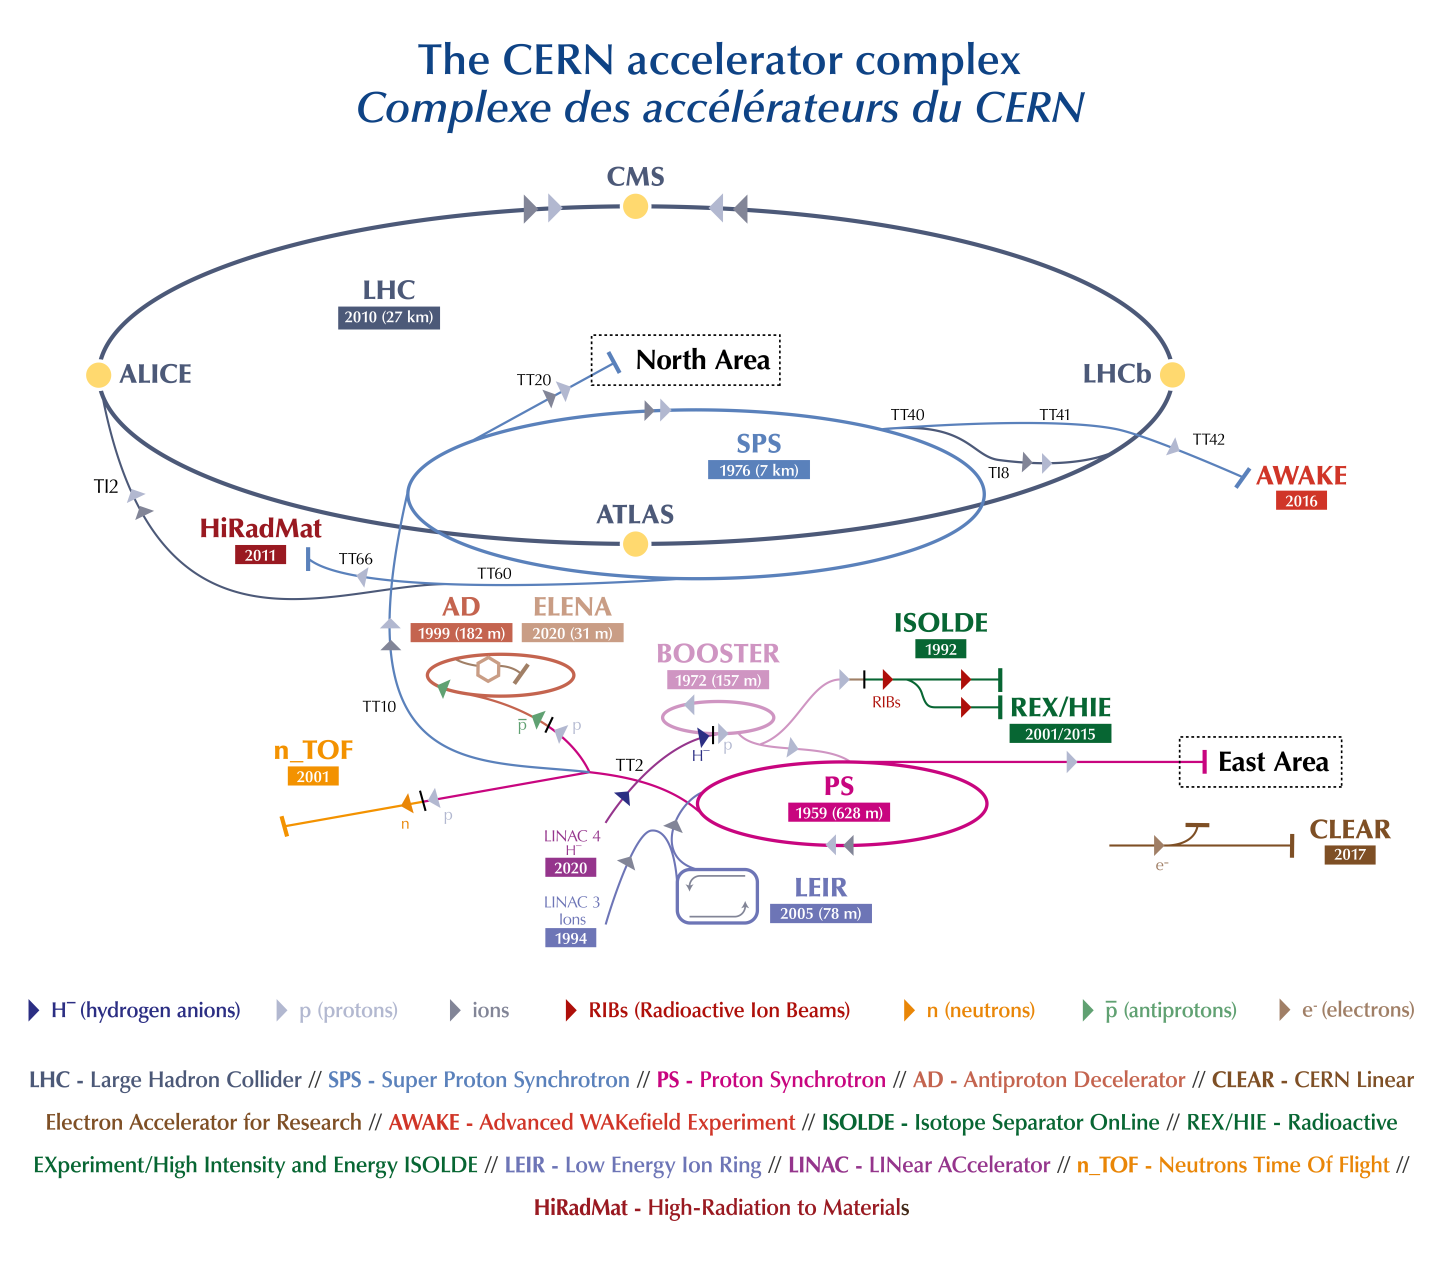
\includegraphics[width=\textwidth]{figures/theoryexperiment/CCC-v2019-final-white}
	\caption{The pre-accelerator complex of the LHC and their corresponding construction years. Accelerator and storage rings are shown in different colours, the particles they accelerate are shown as arrows. Note that the pre-acceleators do not serve the LHC ring exclusively and the diverging paths lead to other independent experiments. Old tunnels of previous experiments serve as pre-accelerators now in the LHC injection chain. \cite{Mobs:2684277}}
	\label{fig:lhcstructure}
\end{figure}

The four main stages of pre-acceleration for protons are listed in \ref{tab:preaccelerators} below. As proton source, hydrogen is used. The protons are first accelerated in the form of H$^-$ ions through the 86 metre long tunnel of the recently (2020) constructed Linear Accelerator 4 (Linac4). Stripped of their pair of electrons, the protons enter the Proton Synchrotron Booster (PSB) where they reach up to \SI{2}{\giga\electronvolt}. In the next step of the injection chain, they enter the Proton Synchrotron (PS), historically the first synchrotron at CERN serving exclusively as a pre-accelerator now. Travelling through the 628 metre long ring and accelerated to 26 GeV, the particles are injected into the Super Proton Synchrotron (SPS), where they are awaiting injection into the LHC once they reach 450 GeV.

\begin{table}[h!]
	\centering
	\begin{tabular}{c|c}
		Accelerator & Peak Energy \\
		\hline
		\hline
		Linear accelerator 4 (Linac4) & 160 MeV \\
		\hline
		Proton Synchrotron Booster (PSB) & 2 GeV \\
		\hline
		Proton Synchrotron (PS) & 26 GeV \\
		\hline
		Super Proton Synchrotron (SPS) & 450 GeV \\
		\hline
		Large Hadron Collider (LHC) & 7 TeV \\
	\end{tabular}
	\caption{The acceleration chain the protons undergo to reach their final energy of 7 TeV.}
	\label{tab:preaccelerators}
\end{table}

\color{red}{Entering the LHC, they live happily forever after until they are brutally crushed into each other and die of quantum mechanics.}\color{black}



\Subsection{The Compact Muon Solenoid}

One of general purpose detectors at the Large Hadron Collider at CERN is the Compact Muon Solenoid (CMS).


% experiment
\pageshift
\thispagestyle{plain}
\Section{Experimental Setup}
\label{ch:experiment}

In this chapter the experimental context of this thesis will be discussed. 

\Subsection{The Large Hadron Collider}
\label{sec:theory}

The Large Hadron Collider (LHC) is currently the most powerful particle accelerator in the world. Hosted at CERN in Geneva at the Swiss-French border and first put into operation on $\text{10}^\text{th}$ September 2008, the LHC is designed for proton and heavy lead ion collisions. The machine has gone through several upgrades between the consecutive data-taking phases (Runs) called Long Shutdowns (LS). During these the proton beam energy has been gradually increased from \SI{3.5}{\tera\electronvolt} to a recently -- on the $\text{5}^{\text{th}}$ July, 2022 to be precise -- achieved energy of \SI{6.8}{\tera\electronvolt} \cite{Alici:2773265} resulting in a total centre-of-mass (CM) proton-proton collision energy of $\sqrt{s} = \SI{13.6}{\tera\electronvolt}$. Similarly, the beam intensity has seen an increase from $1.1 \times 10^{11}$ protons per bunch (ppb) and \textasciitilde200 bunches to a projected \textasciitilde$1.8 \times 10^{11}$ ppb and \textasciitilde2500 bunches \cite{Fartoukh:2790409, Karastathis:2750302}. With a theoretical maximum CM energy of $\sqrt{s} = \SI{14}{\tera\electronvolt}$ and instantaneous luminosity of $L = \SI{10d34}{\centi\meter^{-2}\second^{-1}}$ it holds the record in these measures among concurring experiments.

As a result of consecutive accelerator upgrades, the collider complex has an impressive and complex pre-accelerator structure as shown in fig. \ref{fig:lhcstructure}. Consequently, the proton bunches first go through multiple preparation steps before they get injected into the \SI{27}{\kilo\meter} tunnel of the LHC where the four main experiments (ALICE, ATLAS, CMS and LHCb) and their interaction points are located. 

\begin{figure}[h!]
	\centering
	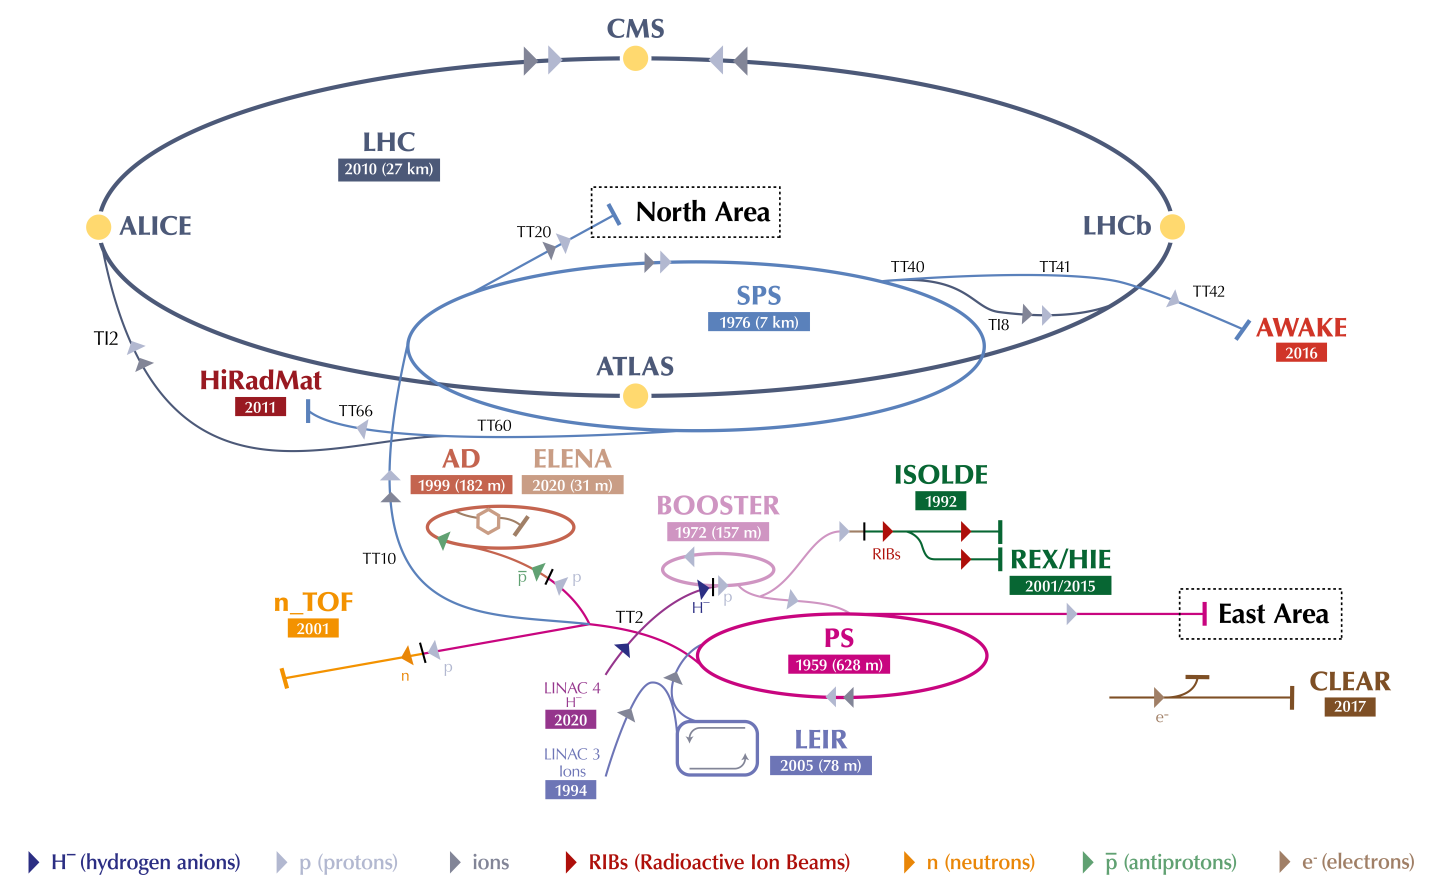
\includegraphics[width=0.8\linewidth]{figures/experiment/CCC-v2019-final-white_cut}
	\caption{The accelerator complex of the LHC, their corresponding construction years and circumferences. Individual stages are shown in different colours, the particle types they accelerate are indicated as arrows. Note that the pre-acceleators do not serve the LHC ring exclusively and the diverging paths lead to other independent experiments. Old tunnels of previous experiments serve as pre-accelerators now in the LHC injection chain. \cite{Mobs:2684277}}
	\label{fig:lhcstructure}
\end{figure}

The four main stages of pre-acceleration for protons are listed in tab. \ref{tab:preaccelerators} below. As proton source, hydrogen is used. The protons are first accelerated in the form of H$^-$ ions through the 86 metre long tunnel of the recently (2020) constructed Linear Accelerator 4 (Linac4). Stripped of their pair of electrons, the protons enter the Proton Synchrotron Booster (PSB) where they reach up to \SI{2}{\giga\electronvolt}. In the next step of the injection chain, they enter the Proton Synchrotron (PS), historically the first synchrotron at CERN serving exclusively as a pre-accelerator now. Travelling through the 628 metres long ring and accelerated to 26 GeV, the particles are injected into the Super Proton Synchrotron (SPS), where they are awaiting injection into the LHC once they reach 450 GeV.

%https://home.cern/science/accelerators/linear-accelerator-4
%https://home.cern/science/accelerators/proton-synchrotron-booster
%https://home.cern/science/accelerators/proton-synchrotron
%https://home.cern/science/accelerators/super-proton-synchrotron
%https://home.cern/science/accelerators/large-hadron-collider

\begin{table}[h!]
	\centering
	\begin{tabular}{c|c}
		Accelerator & Peak Energy \\
		\hline
		\hline
		Linear accelerator 4 (Linac4) & 160 MeV \\
		\hline
		Proton Synchrotron Booster (PSB) & 2 GeV \\
		\hline
		Proton Synchrotron (PS) & 26 GeV \\
		\hline
		Super Proton Synchrotron (SPS) & 450 GeV \\
		\hline
		Large Hadron Collider (LHC) & 7 TeV \\
	\end{tabular}
	\caption{The acceleration chain the protons undergo to reach their final energy of 7 TeV.}
	\label{tab:preaccelerators}
\end{table}

In the LHC the beams are circulating in opposing directions. They are kept on a circular trajectory using superconducting NbTi magnets operating at \SI{1.9}{\kelvin} thanks to the superfluid helium bath at about \SI{0.13}{\mega\pascal} \cite{Bruning:782076}. In the tunnel itself there are eight interactions points (IP). ATLAS, ALICE, CMS and LHCb are located at IP1, IP2, IP5 and IP8, respectively. IP3 and IP7 are where the momentum and betatron collimators are located ensuring beam quality; the radiofrequency (RF) cavities are at IP4 increasing the bunch energy to 7 TeV. The beam dump is at IP6 where old bunches are deflected by the fast-pulsing "kicker" magnets and directed towards the carbon absorber at the end of their lifetime. \cite{Evans_2008}

\begin{figure}[h!]
	\centering
	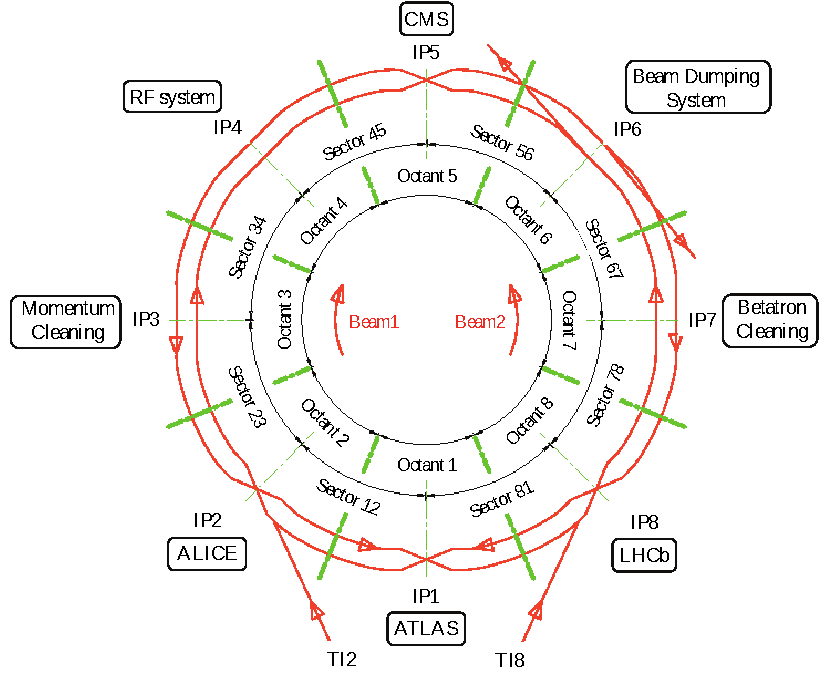
\includegraphics[width=0.6\linewidth]{figures/experiment/LHC_ring.pdf}
	\caption{The location of the interaction points, the experiments, and the beam adjustment systems. The LHC ring is also divided into further sectors and octants for each IP. \cite{Bracco:1174254}}
	\label{fig:LHC_ring}
\end{figure}

The four main detectors perform the particle collision measurements. LHCb specializes on flavour physics and measures b-quark decays focussing on the measurement and study of CP-violating processes. ALICE has been constructed to mainly study the quark-gluon plasma resulting from heavy ion collisions. ATLAS and CMS are sister experiments and are general purpose detectors. In the following, the latter will be described in detail only.

\Subsection{The Compact Muon Solenoid}

The Compact Muon Solenoid (CMS) detector is a 14 000 tonnes heavy detector measuring 28.7 metres in lenght and 15.9 metres in diameters. It has been built to be general purpose detector, featuring additional muon chambers at its most outer side allowing the precise measurement of muon momenta. The detector is built around a solenoid magnet, producing a magnetic field of $\SI{4}{\tesla}$. CMS has several subdetector components which surround the beampipe in a layered, onion-like structure. CMS has rotational symmetry around the beam pipe along which the z-axis is usually defined. The positions of each components and some of their most important technical details are shown in fig. \ref{fig:cms_view}.

\begin{figure}[h!]
	\centering
	\includegraphics[width=0.8\linewidth]{figures/experiment/cms_160312_02.pdf}
	\caption{The inner structure of the CMS detector. Note the layered structure and rotational symmetry of the detector. Each layer performs an individual step in particle identification. \cite{Sakuma:2665537}}
	\label{fig:cms_view}
\end{figure}

The coordinate system has its origin at the interaction point, is right-handed, with the $z$-axis pointing towards the anti-clockwise beam direction. Hence, the $xy$ plane lies orthogonal to the beam pipe. Instead of the polar angle directly the pseudorapidity 

\begin{equation*}
	\eta = -\ln\tan\frac{\theta}{2}
\end{equation*}

is used, as it is an Lorentz-invariant quantity along the beam. $\eta = \pm\infty$ hence corresponds to the beampipe and $\eta = 0$ defines the $xy$ (transversal) plane. Using the pseudorapidity, the differences in the $\eta-\phi$ plane can be given by

\begin{equation*}
	\Delta R = \sqrt{\left(\Delta\eta\right)^2 + \left(\Delta\phi\right)^2}
\end{equation*}

With that, particle kinematics can be described in terms of their energy $E$, the transversal momentum $p_T$, $\eta$, $\phi$ and their mass $m$. In some cases, instead of the pseudorapidity, the rapidity

\begin{equation*}
	y = \frac{1}{2}\ln\frac{E+p_z}{E-p_z}
\end{equation*}

is used.

In the following, the main subdetector components, their location and role focussing on high $p_T$ events will be briefly described.

\Subsubsection{Silicon Tracking}

CMS has an all-silicon tracking system, which lies at the core of the detector close to the beam pipe. As the name suggests, the tracking system enables the reconstruction of the trajectories of the child particles passing through the detector. It thus plays a crucial role in particle identification as the charge of particles can be inferred from the track signature (or the lack thereof); apart from that, it also enables secondary vertex reconstruction of short-living primary particles. Particles passing through the silicon ionize the tracker, producing a signal.

Having a length of 5.4 metres and a diameter of 2.4 metres it covers the pseudorapidity range $|\eta|<2.5$, the best tracking efficiency being in the barrel region $|\eta| < 0.9$ \cite{Veszpremi_2014}. Closest to the interaction point lies the pixel silicon tracker. Made-up of four cylindrical layers at $\SI{3}{\centi\meter}$, $\SI{7}{\centi\meter}$, $\SI{11}{\centi\meter}$ and $\SI{16}{\centi\meter}$ from the beam pipe at disks at the end, it is segmented into 124 million pixels of $\SI{100}{\micro\meter} \times \SI{150}{\micro\meter}$ and kept at $\SI{-20}{\degreeCelsius}$ during operation.

Outside of the silicon pixel detector lie the silicon strip detectors, which is divided into four parts: the inner barrel par (TIB), the inner disk part (TID), the outer barrel (TOB) and the outer endcap part (TEC). This part of the tracker contains about 10 million strip components. The complete layout of the strip detectors is shown in fig. \ref{fig:strip_tracker}.

\begin{figure}[h!]
	\centering
	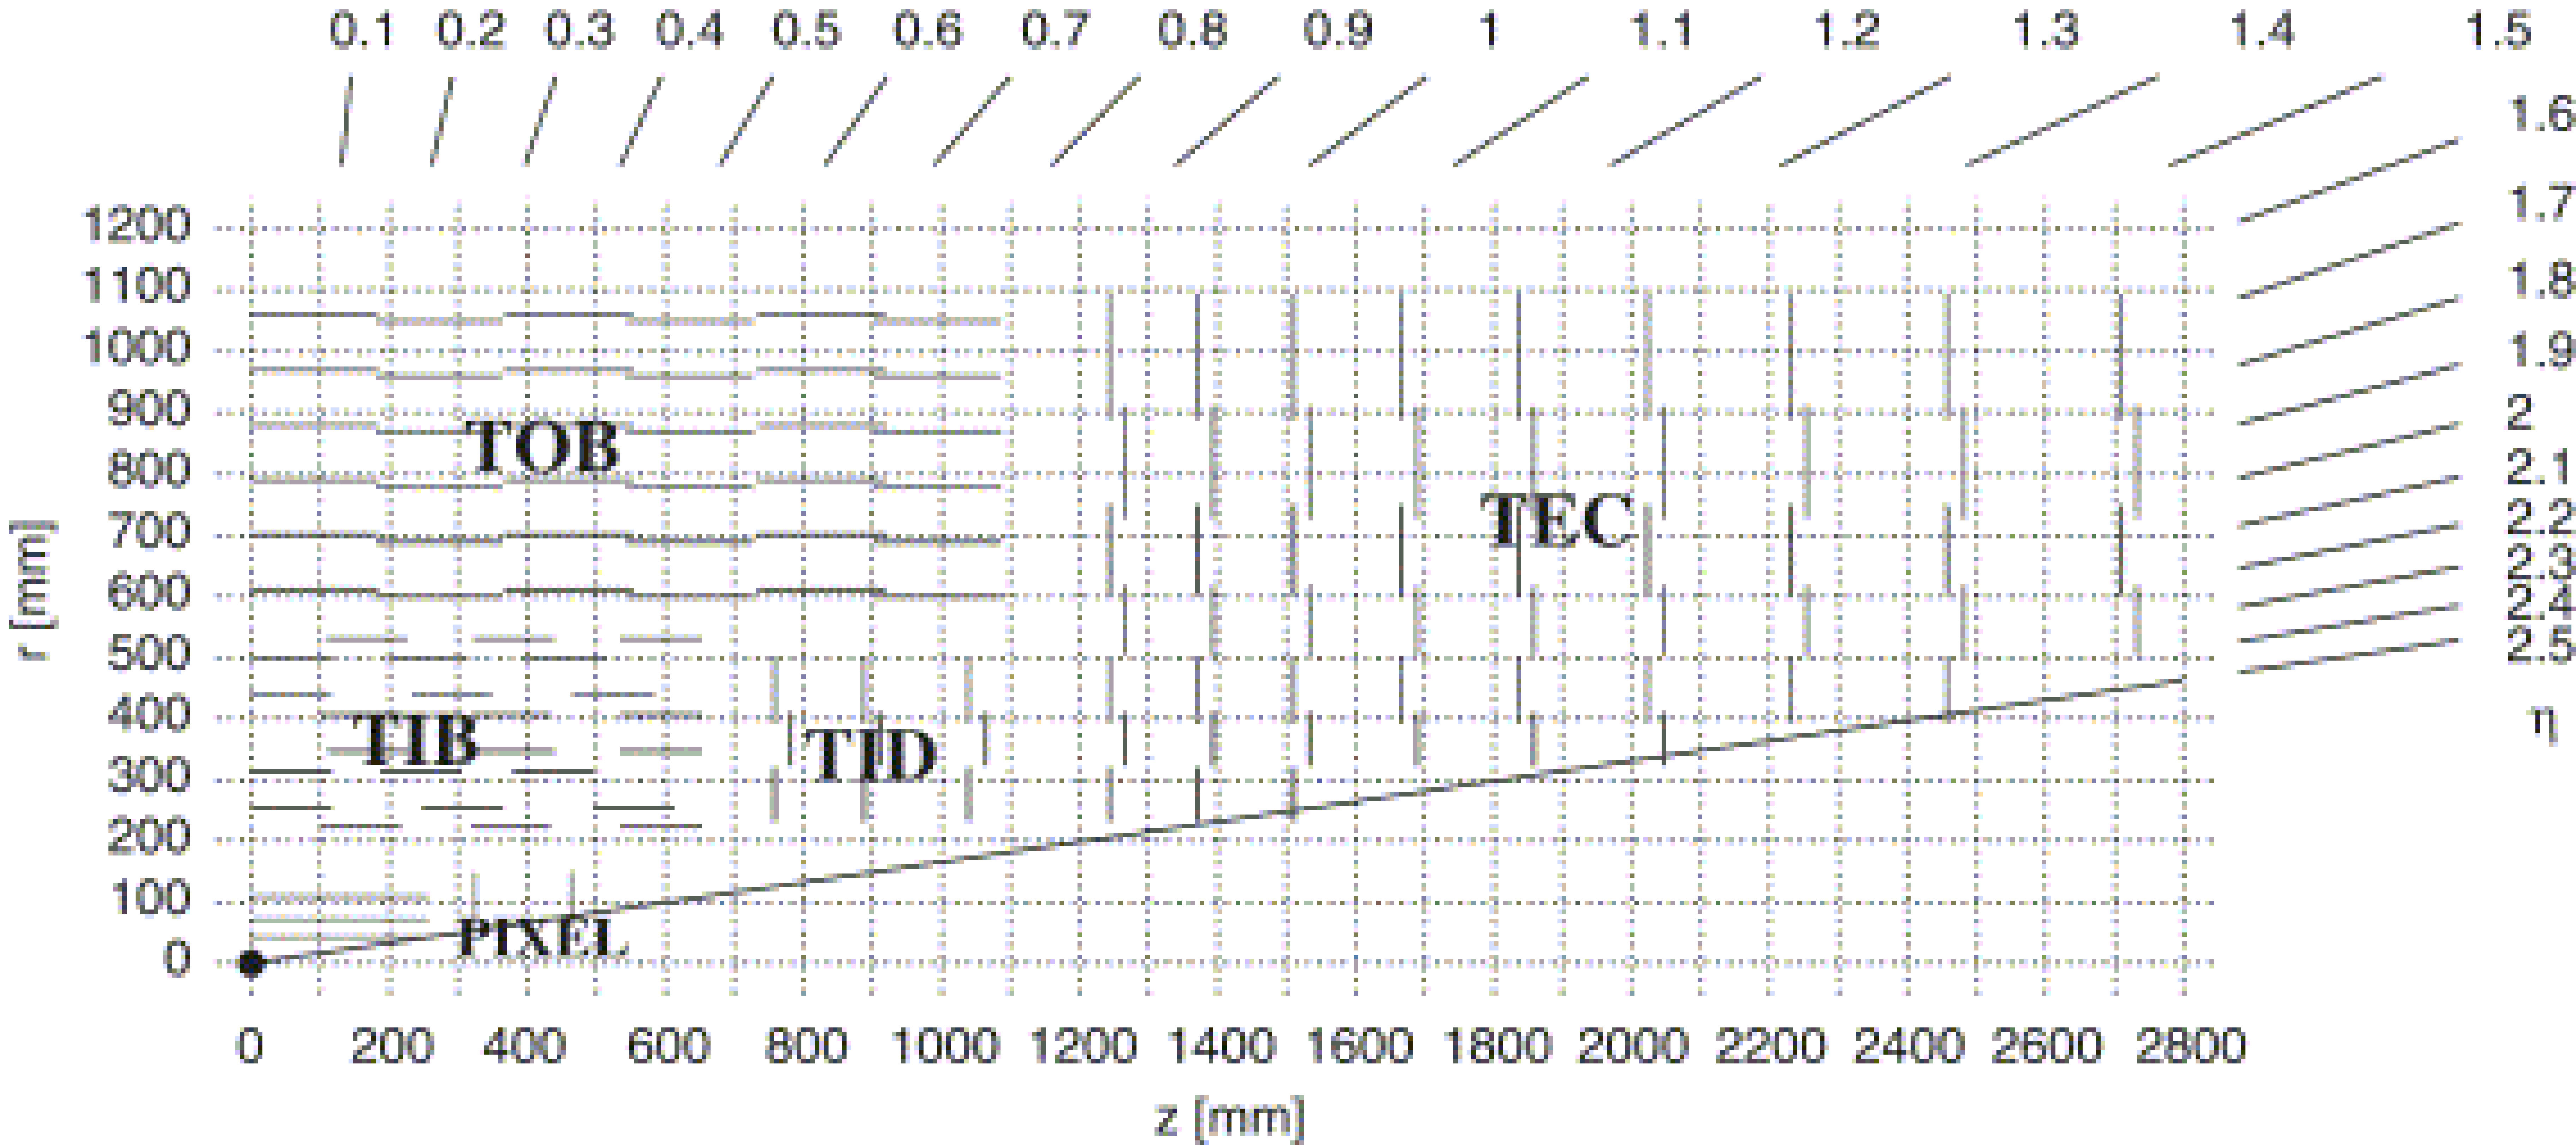
\includegraphics[width=0.8\linewidth]{figures/experiment/StripTracker}
	\caption{View of one quarter of the silicon strip detectors in the $r-z$ plane, indicating both the geometry and the pseudorapidity range of the individual parts. \cite{Azzurri:914891}}
	\label{fig:strip_tracker}
\end{figure}

\Subsubsection{Electromagnetic Calorimeter}

The CMS electromagnetic calorimeter (ECAL) measures the energy of electrons and photons by absorbing them completely and measuring the induced particle shower during that. It lies outside of the tracking system and consists of highly transparent and scintillating lead tungstate (PbWO$_4$) crystals. The ECAL consists of two components as well, and central barrel (EB) covering the region up to $|\eta| = 1.48$ and an endcap region (EE) extending this coverage to pseudorapidities of $|\eta| = 3.0$ \cite{Biino_2015}. The EB has 61 200 crystals, which are formed into modules weighing around $\SI{3}{\tonne}$ and containing 1700 crystals, which are $\SI{23}{\centi\meter}$ (or $25.8 X_0$ in terms of radiation length $X_0$) in length. The EC and the end of the barrel modules have almost 15 000 more crystals; the total volume of the crystals is $\SI{11}{\cubic\meter}$ with a weight of $\SI{92}{\tonne}$. The layout of the calorimeter structure is shown in fig. \ref{fig:ecal}.

\begin{figure}[h!]
	\centering
	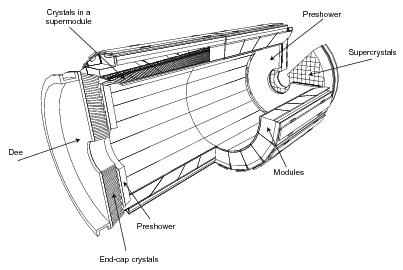
\includegraphics[width=0.6\linewidth]{figures/experiment/ecal.png}
	\caption{Schematic view of the CMS barrel and endcap calorimeters. Note the coverage around the tracker (not shown explicitly) and the preshower module, responsible for better seperation of photon hits in the endcap region. \cite{Chatrchyan:1554142}}
	\label{fig:ecal}
\end{figure}

The energy resolution of the barrel calorimeters has tree terms: a stochastic, a noise and a constant term and was measured to be \cite{Chatrchyan:1554142}

\begin{equation*}
	\frac{\sigma_E}{E} = \underbrace{\frac{2.8\%}{\sqrt{E\left[GeV\right]}}}_\text{stochastic} \oplus \, \underbrace{\vphantom{\frac{2.8\%}{\sqrt{E\left[GeV\right]}}}\frac{12\%}{E\left[GeV\right]}}_\text{noise} \oplus \, \underbrace{\vphantom{\frac{2.8\%}{\sqrt{E\left[GeV\right]}}}0.3\%}_\text{constant}
\end{equation*}

%In the barrel region the crystals are equipped with avalanche photodiodes (APD) of $5 \times \SI{5}{\square\milli\meter}$ and they are insensitive to the $\SI{4}{\tesla}$ magnetic field in the detector.

\Subsubsection{Hadronic Calorimeter}

The CMS hadronic calorimeters (HCAL) is a sampling calorimeter. Similarly to the ECAL, its purpose is to measure the energy of hadrons by measuring the induced avalanche of secondary particles upon passing through the detector as they are not directly stopped in the ECAL. In the $|\eta|<3$ region it consists of a brass scintillator calorimeter; in the forward region $3<|\eta|<5$ in has a iron quartz-fiber calorimeter \cite{canko_ak_2009}. It is organized into barrel (HB), outer barrel (HO), endcap (HE) and forward (HF) regions. The layout and the positioning of the respective components are shown in fig. \ref{fig:hcal}. Combined with the ECAL, the HCAL measures jets with a resolution of \cite{Lopez}

\begin{equation*}
	\frac{\sigma_E}{E} = \frac{100\%}{\sqrt{E\left[GeV\right]}} \oplus 5\%
\end{equation*}

\begin{figure}[h!]
	\centering
	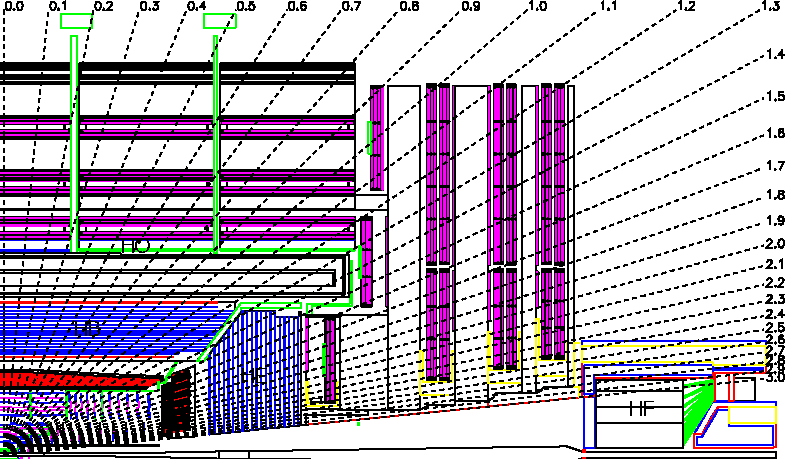
\includegraphics[width=0.8\linewidth]{figures/experiment/hcal.pdf}
	\caption{The CMS HCAL module setup. Note that the outer calorimeter lies outside of the solenoid (the white rectangle between HB and HO). \cite{Chatrchyan:1129810}}
	\label{fig:hcal}
\end{figure}

\Subsubsection{Superconducting Solenoid Magnet and the Return Yokes}

A core component of the detector is the solenoid magnet itself. Weighing $\SI{12000}{\tonne}$ and cooled down to $\SI{-268.5}{\degreeCelsius}$ it can produce a magnetic field of $\SI{4}{\tesla}$ ($\SI{3.8}{\tesla}$ during the runs), it is the largest solenoid in the world. The solenoid magnet and the return yokes play a crucial role in particle identification and muon measurement. These high magnetic fields are achieved using NbTi coils and a current of $\SI{18160}{\ampere}$. Outside of the solenoid magnet itself lie the muon chambers and the five return yokes, which are constructed from steel. The field strength thanks to the yokes there is around $\SI{2}{\tesla}$.

\Subsubsection{Muon Chambers}

In the outermost layers of the detector, the muon chambers can be found. CMS specializes in muon measurements and these chambers are characteristic for the whole detector. As muons provide a clear signature (like in a $H \rightarrow ZZ \rightarrow \mu\mu\mu\mu$, which is referred to as the "Golden Channel"), their reconstruction is highly motivated. Due to muons having several orders of magnitude higher mass compared to electrons, they can pass the ECAL and they are not stopped by it.  Hence, they do not deposit their complete energy there meaning they can escape all the inner detector components. For this reason, additional measurements on their momenta are needed.

The chambers have four subcomponents: the drift tubes (TB), the cathode strip chambers (CSCs), the resistive plate chambers (RPCs) and the gas electron multipliers (GEMs), all of which are gaseous detectors. In the region $|\eta|<1.2$ the four layers of drift tubes have been installed at a radius of approximately $\SI{4}{\meter}$, $\SI{4.9}{\meter}$, $\SI{5.9}{\meter}$ and $\SI{7}{\meter}$. The tubes consist of 250 chambers and looking from the transversal plane, they are grouped into 12 sectors, with each covering 30° azimuthal angle. These chambers are staggered in a way, such that a high $p_T$ muon produced a the sector boundary crosses at least 3 of the four layers. In the endcap region up to $|\eta| < 2.4$, the CSCs are deployed. The CSCs are used both in the endcap and the barrel region. The newly added GEMs have been installed in the region $1.6 < |\eta| < 2.2$ \cite{Colaleo:2021453}. The exact position of the components are shown in fig. \ref{fig:muonchambers}.

\begin{figure}[h!]
	\centering
	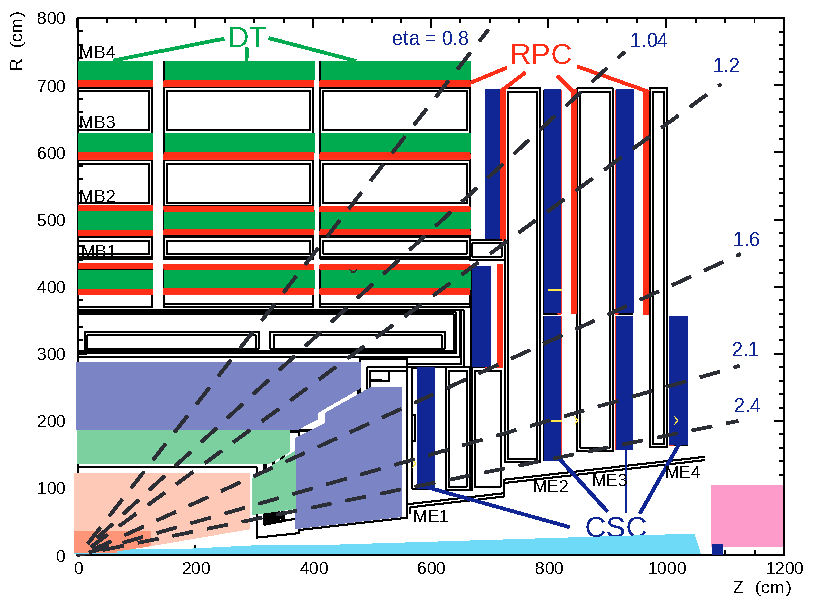
\includegraphics[width=0.8\linewidth]{figures/experiment/muonchambers.pdf}
	\caption{The location of the drift tubes (DT), the cathode strip chambers (CSCs) the resistive plate chambers (RPCs). The newly deployed GEMs are in the region $1.6 < |\eta| < 2.2$ (not shown here) \cite{Bayatian:922757}.}
	\label{fig:muonchambers}
\end{figure}

\Subsubsection{Trigger System}

With a collision frequency of $\SI{40}{\mega\hertz}$ with a new collision in every $\SI{25}{\nano\second}$ it is both impossible and unnecessary to record every event in the detector; impossible because the complete registration of this enormous data-flow is technologically impossible and unnecessary as most of these events arise from soft collision processes. For this reason, a filtering (triggering) mechanism has been implemented in the detector.

The trigger system reduces the dataflow in two steps. The Level-1 (L1) trigger operates on a hardware level and reaches a decision in less than $\SI{1}{\micro\second}$. During the decision-making period, the high-resolution data is held the memory and increasingly complex algorithms are used to approach the quality of final reconstruction. These decisions involve information from the calorimeters and the muon systems and some correlation between them. It is based mostly on jet $E_T$ and $p_T$ thresholds and physics objects like photons, electrons and muons. The resulting data-stream from the L1 trigger is less than $\SI{100}{\kilo\hertz}$.

In the second step, the High-Level Triggers continue with the processing. They operate on a software level and have an output rate of $\SI{100}{\hertz}$ which can be stored offline for further analysis. Instead of fully reconstructing events from every detector component, they are first only partially reconstructed and eventually discarded as soon as possible \cite{Bayatian:922757}.

\Subsection{Physics Object Reconstruction}
\Subsubsection{Particle Flow}

Individual particles leave (up to the detector resolution) unique event signatures in each subdetector component, which is summarized in fig. \ref{fig:cms_slice}. In order to perform a complete physics analysis, these event signatures have to be assigned to physically interpretable objects in order to obtain the physical final state and kinematics such as energy, momenta and charge.

\begin{figure}[h!]
	\centering
	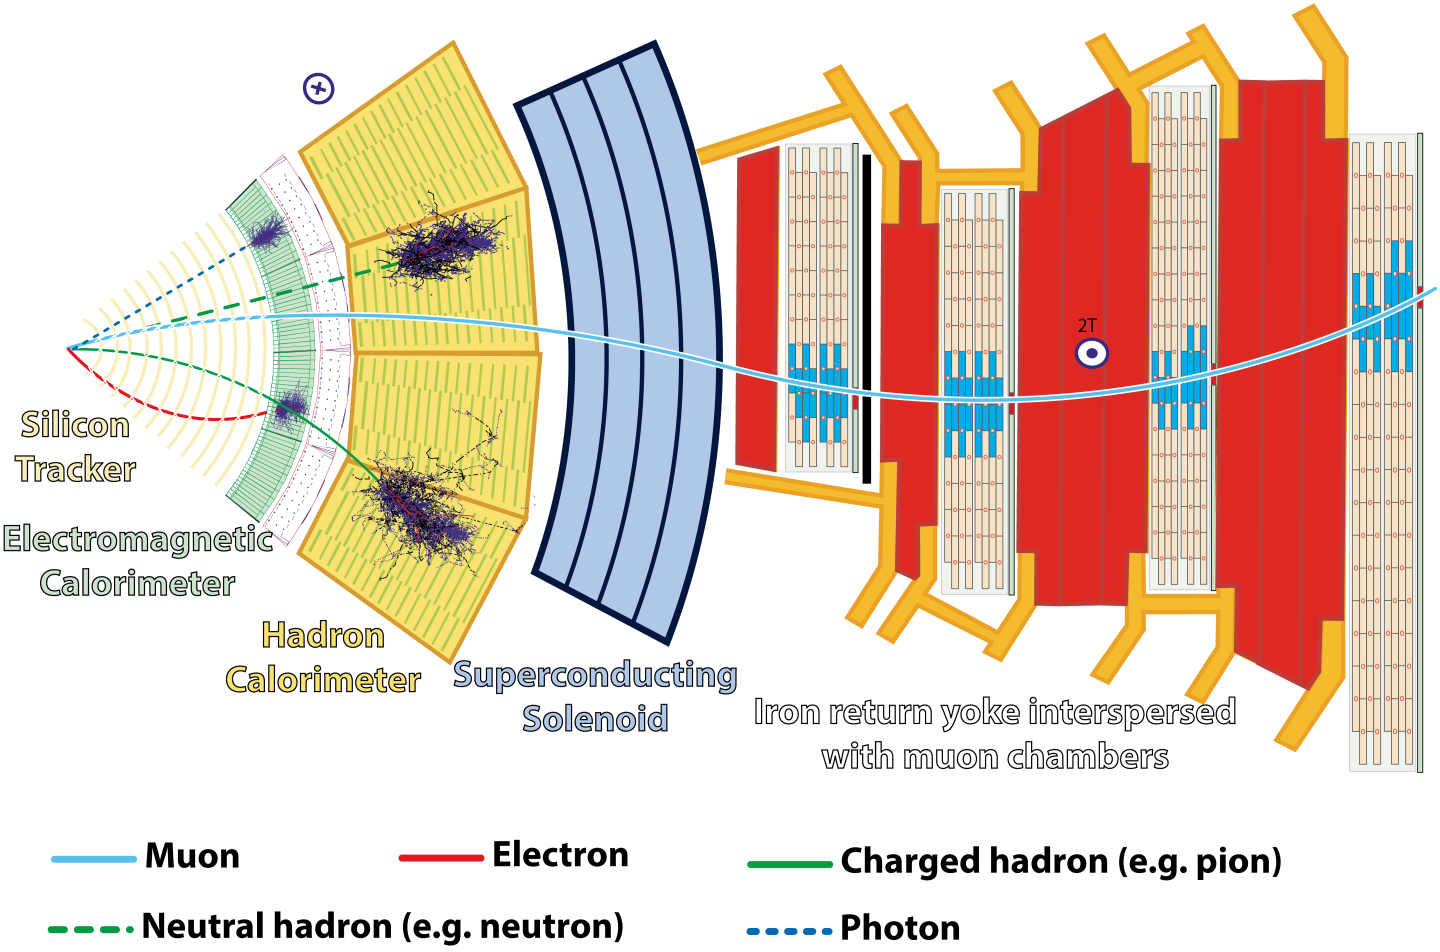
\includegraphics[width=0.8\linewidth]{figures/experiment/CMS_Slice}
	\caption{Transversal view of a slice of the CMS detector with several characteristic signatures drawn in different colours. Note that each detector slice functions as a filter for different particle kinds, i.e. the number of signatures decreases towards the outer layers. \cite{Barney:2120661}}
	\label{fig:cms_slice}
\end{figure}

The reconstruction algorithm used at the CMS experiment is Particle Flow (PF) \cite{Sirunyan_2017}. In order to obtain the physics objects, it first combines the particle tracker hits (both from the tracker and from the muon chambers) and clusters the energy deposits in the calorimeters. In order to keep the number of misreconstructed tracks minimal during track reconstruction several quality fit criteria are relaxed with each iteration. For the calorimeter clusters, an expectation-maximization algorithm based on a Gaussian-mixture model is used to reconstruct the clusters within the computed topological clusters around the pre-constructed cluster seeds.

Following that, the link algorithm is executed which connects the aforementioned PF elements from different subdetectors. At this point, it cannot be avoided that some particles are misidentified or wrongly reconstructed, especially in cases where a large missing transverse momentum $p^{miss}_T$ is present in the event. As such events (usually originating from misreconstructed high $p_T$ muons) may be wrongly selected by a large set of new physics searches, they undergo a post-processing algorithm in order to correct these effects.

Finally, the reconstructed particles are used to build the physics objects, namely jets, missing transverse momenta $p^{miss}_T$, muon, electrons and taus and other related quantities. Note that as a hadron collider, the exact centre-of-mass system is a priori unknown due to the interacting partons within the proton structure, hence the missing momenta can only be evaluated in the transversal plane.

\Subsubsection{Jet Clustering}

The hadronisation and fragmentation processes give rise to an avalanche of secondary particles in the detector called jets. Their reconstruction requires sophisticated tools to assign the detector hits to specific clusters. Such algorithms should ideally satisfy two requirements: they should be infrared and collinear safe, i.e. they should not be disturbed by soft emmisions (particles with low momenta) while collinear particles belonging to the same jet should be assigned correctly. CMS uses the anti-$k_T$ algorithm, a generalization of the $k_t$ and Cambridge/Aachen algorithm \cite{Cacciari_2008}. They are given by\footnote{Setting $p=0$ yields the Cambridge/Aachen algorithm, while $p=1$ one recovers the $k_t$ algorithm.}

\begin{equation*}
	\begin{aligned}
		d_{ij} &= \min\left(k^{2p}_{ti}, k^{2p}_{tj}\right)\frac{\Delta^2_{ij}}{R^2} \\
		d_{iB} &= k^{2p}_{ti}
	\end{aligned}
\end{equation*}

where $\Delta^2_{ij} = (y_i-y_j)^2 + (\phi_i - \phi_j)^2$ is the distance in the plane spanned by the rapidity $y$ and the azimuthal angle $\phi$ between particles $i$ and $j$, $R$ is a radius parameter, $k_{ti}$ is the transverse momentum of particle $i$ and $d_{iB}$ is the distance between the particle and the beam. Setting the parameter $p$ to $p=-1$ results in the both infrared, collinear safe and fast anti-$k_t$ algorithm.

Anti-$k_t$ accumulates soft particles which are in a radius $R$ of a hard particle if no other hard neighbours are present within $2R$  to the hard particle themselves in a perfectly conical jet. If there is another hard particle with $R < \Delta<2R$, then two not necessarily conical jets will be returned; for $\Delta<R$, both particles will form a single jet. From here one can see the stability of the algorithm with respect to soft emmisions while maintaining collinear safety.

One can differentiate two kinds of jets by setting the radius $R$. Picking $R=0.4$ or $R=0.8$ results in AK4 or AK8 jets, respectively. Nevertheless, the quark flavour which produces the jet cannot simply be obtained by jet clustering. Consequently, the quark flavour identification (flavour tagging) has to be performed separately.

\Subsubsection{Flavour Tagging}

Assigning flavour to the jet-inducing quarks is possible through several heavy-flavour jet discriminating variables, which can be reconstructed by deep neural networks \cite{Sirunyan_2018}.

For b quarks, the displacement of the secondary vertex due to the long enough lifetime of b hadrons which is at the order of $\SI{1.5}{\pico\second}$ (which corresponds to displacements of a few mm to $\SI{1}{\centi\meter}$) can be reconstructed. These displacements can be resolved with the tracker and can be characterized by the impact parameter (which is defined as the vector pointing from the primary vertex to the point of closest approach) of the child particles. Due to the heavier mass of the b and c quarks, the decay products have a larger transversal momentum with respect to the jet axis yielding larger impact parameter vectors compared that of their light counterparts. In addition to that, in approximately 20\% and 10\% of the cases in the decay chain of b and c hadrons, respectively, a muon or an electron is present, which can further be used for heavy-flavour jet identification.

\begin{figure}[h!]
	\centering
	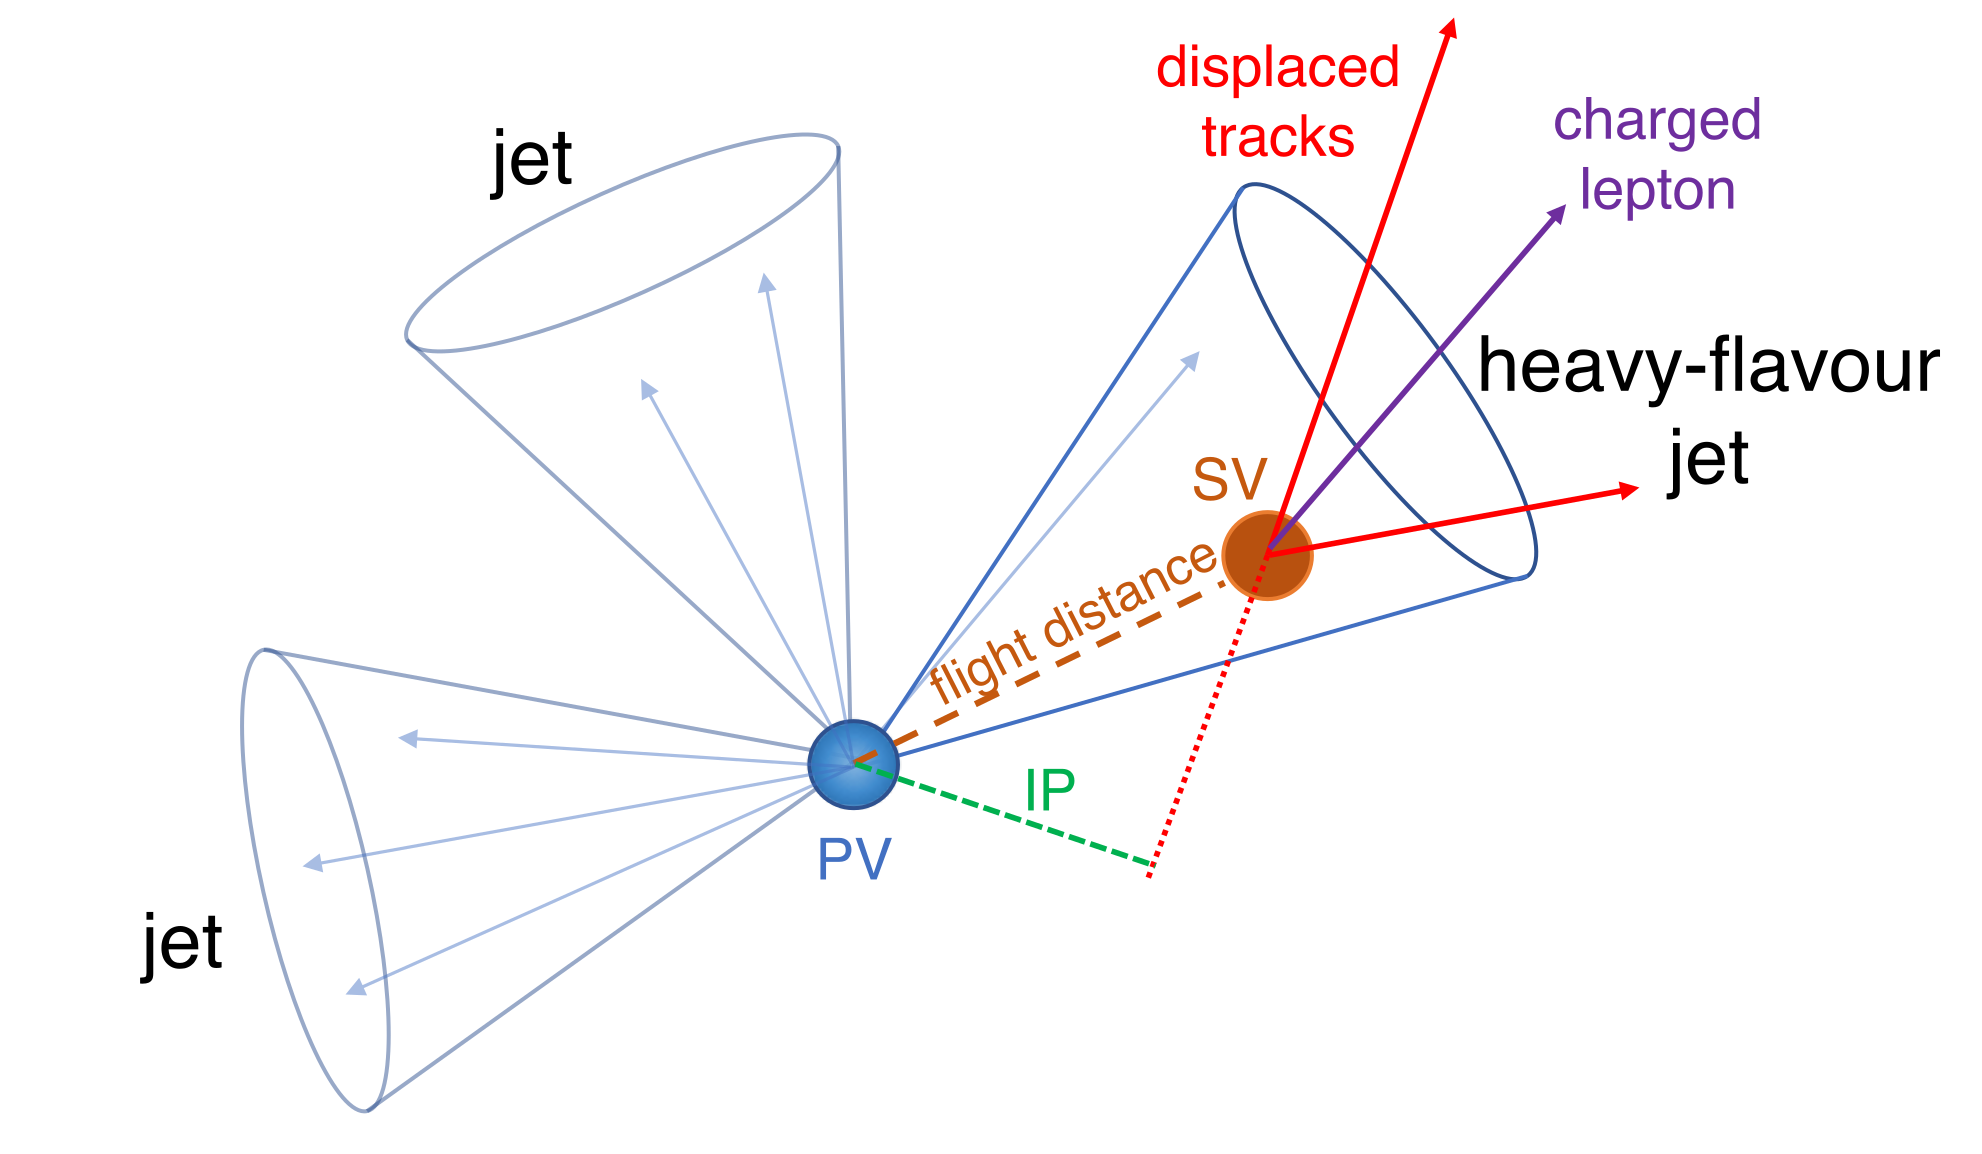
\includegraphics[width=0.6\linewidth]{figures/experiment/pvsv}
	\caption{Schematic view of the displacement of the secondary vertex with respect to the primary vertex with the definition of the impact parameter indicated. Note the possible appearence of a soft lepton (shown in purple) in the jet cone characteristic for heavy-flavour jets.}
	\label{fig:pvsv}
\end{figure}

\Subsubsection{Muons}

Since muons can leave signatures in both the tracker and the muon system, they are reconstructed and categorized depending on the muon signal quality and their physics properties. For the track reconstruction, the three categories in increasing quality are: \cite{Collaboration_2010}

\begin{itemize}
	\item[] \textit{Standalone-muon tracks} are constructed from the CSC, RPC and DT signatures using a Kalman-filter technique.
	\item[] \textit{Tracker muon tracks} are built "from the inside out" by loose matching tracker tracks (with $p_T > \SI{0.5}{\giga\electronvolt}$ and a total momentum of $p>\SI{2.5}{\giga\electronvolt}$) to DT and CSC segments. tracks automatically qualify if at least one muon segment matches the extrapolated track.
	\item[] \textit{Global muon tracks} are obtained "outside-in" by matching the standalone-muon tracks with the tracker tracks with the Kalman filter.
\end{itemize}

Note that these categories are not exclusive. Thanks to the high resolution and efficiency of muon track reconstruction, approximately 99\% of the muons are reconstructed as either as a tracker track muon, global muon track or both.

Following the categorization by the tracks, the muon IDs are assigned \cite{Sirunyan_2018_muons}. Using the variables from the track fit, the following identification types are assigned:

\begin{itemize}
	\item[] \textit{Loose muon ID} are for muons selected by the PF algorithm which is either a tracker or global muon. This selection ensures the identification of prompt muons originating from the primary vertex or from light and heavy flavour decays while minimizing the rate of charged hadrons misidentified as muons.
	\item[] \textit{Medium muons} are prompt muons and muons from heavy flavour decays which carry the loose ID with tracker track hits of more than 80\% of the inner tracker layers.
	\item[] \textit{Tight muon IDs} suppress hadronic punch-through and muons from decay in flight. They are both tracker and global muons with at least pixel hit and hits from at least six inner layer tracker hits, fulfilling additional event geometric criteria.
	\item[] \textit{Soft muons} are low $p_T$ muons with high purity tracker track of the same tracker requirements as tight muons.
	\item[] \textit{High momentum muon IDs} are for muons with $p_T > \SI{200}{\giga\electronvolt}$. They are both tracker and global muons with the same tracker hit and event geometric requirements as tight muons. In addition to that, they need at least one hit from the muon system for the global muon.
\end{itemize}

% deep learning
\pageshift
\thispagestyle{plain}
\Section{Deep Learning and Conditional Invertible Neural Networks}
\label{ch:deeplearning}

Deep Learning is a subdomain within Machine Learning focusing on the construction and training of deep neural networks. Such networks have been proven to be extremely successful in different, analytically unsolvable problems such as (but not restricted to) image classification tasks, regression tasks, image generation tasks, language translation and reinforcement learning.

In this chapter, a brief introduction to these networks and their properties with a focus on so-called normalizing flows and invertible neural networks is given.

\Subsection{Foundations of Deep Learning and Neural Networks}
\Subsubsection{The Universal Approximation Theorem}

The success of Neural Networks (NNs) lies in their potential of learning (almost) arbitrary models. This property of NNs can be expressed mathematically through the Universal Approximation Theorem which in words states a feed-forward network with linear output and at least one hidden layer with a finite number of nodes can approximate any real continuous function on a given closed and bounded subset to arbitrary precision \cite{DLiPR}.

However, the Universal Approximation Theorem does not state how the network should be constructed to achieve the desired precision. For this reason, the theorem has been proven for several network architectures; in case of ReLU-activated feed-forward networks the theorem can be written as the following \cite{UAC}:
\newtheorem{theorem}{Theorem}
\begin{theorem}
	For any real and continuous function $f : [0, 1]^{d_{in}} \rightarrow \mathbb{R}^{d_{out}}$ and every $\epsilon>0$ there is a ReLU-network $\mathcal{N}$ with the same input and output dimension $d_{in}$ and $d_{out}$ and a minimum hidden layer width $w_{min}$ for which
	\begin{equation*}
		\sup_{x\in[0, 1]^{d_{in}}}\Vert f(x)-f_\mathcal{N}(x)\Vert \leq \epsilon
	\end{equation*}
	and
	\begin{equation*}
		d_{in} + 1 \leq w_{min}(d_{in}, d_{out}) \leq d_{in} + d_{out}
	\end{equation*}
\end{theorem}
This theorem does not state anything about the exact depth (number of layers) the network needs to have, its speed of convergence and the optimization process it needs to undergo to achieve this arbitrary approximation. On the other hand, it is reassuring to have a mathematical guarantee for convergence for a given feed-forward network structure. For this reason, empiric studies are usually performed to look for a locally optimal solution for a given task.

In the following, a brief overview of the most common NN components is going to be given with special focus on the ones used for the construction of the cINN.

\Subsubsection{Fully-Connected Neural Networks}
The most elementary NNs perform affine transformations (consisting of a linear transformation represented by a weight matrix $W$ and a shift $b$) on a given input $x$ followed by the application of a non-linear function (called activation) $g$:

\begin{equation*}
	y = g(Wx+b)
\end{equation*}

Graphically, one such transformation is represented as a layer. For a fully-connected neural network, these transformations are called in succession, resulting in stacked layers of $n$ nonlinearities as shown in fig. \ref{fig:nn}. The resulting mapping

\begin{equation*}
	f(x, \theta) = g^n\left\{W^{n-1}g^{n-1}\left[ ... \left(W^2g^1(W^1x+b^1)+b^2\right)...\right]+b^{n-1}\right\}
\end{equation*}

is a universal approximator with the free parameters $\theta$ (containing all the matrices $W^i$ and the biases $b^i$) for the target output for $y$. Finding the optimal parameters $\theta$ is called training and the $\theta$ will be referred to as trainable parameters. The graphical representation of a neural network mapping is shown in fig. \ref{fig:nn}.

\tikzset{%
	every neuron/.style={
		circle,
		draw,
		minimum size=1cm
	},
	neuron missing/.style={
		draw=none, 
		scale=2.5,
		text height=0.333cm,
		execute at begin node=\color{black}$\vdots$
	},
}
\begin{figure}[h!]
	\centering
	\begin{tikzpicture}[x=1.5cm, y=1.5cm, >=stealth]
		
		\foreach \m/\l [count=\y] in {1,2,missing,3}
		\node [every neuron/.try, neuron \m/.try] (input-\m) at (0,2.5-\y) {};
		
		\foreach \m [count=\y] in {1,missing,2}
		\node [every neuron/.try, neuron \m/.try ] (hidden-\m) at (2,2-\y) {};
		
		\foreach \m [count=\y] in {1,missing,2}
		\node [every neuron/.try, neuron \m/.try ] (output-\m) at (4,2-\y) {};
		
		\foreach \l [count=\i] in {1,2,n}
		\draw [<-] (input-\i) -- ++(-1,0)
		node [above, midway] {$I_\l$};
		
		\foreach \l [count=\i] in {1,n}
		\node [above] at (hidden-\i.north) {$H_\l$};
		
		\foreach \l [count=\i] in {1,n}
		\draw [->] (output-\i) -- ++(1,0)
		node [above, midway] {$O_\l$};
		
		\foreach \i in {1,...,3}
		\foreach \j in {1,...,2}
		\draw [->] (input-\i) -- (hidden-\j);
		
%		\foreach \i in {1,...,2}
%		\foreach \j in {1,...,2}
%		\draw [->] (hidden-\i) -- (output-\j);
%		\draw [->] (hidden-1) -- (output-1);
%		\draw [->] (hidden-2) -- (output-2);
		
		\foreach \l [count=\x from 0] in {Input\\ layer, Hidden\\ layers, Ouput\\ layer}
		\node [align=center, above] at (\x*2,2) {\l};
		
		\node [draw=none, scale=2.5, text height=0.333cm] at (3, 0) {$\ddots$};
		\node [draw=none, scale=2.5, text height=0.333cm] at (3, 1.25) {$\hdots$};
		\node [draw=none, scale=2.5, text height=0.333cm] at (3, -0.75) {$\hdots$};
		
	\end{tikzpicture}
	\caption{Schematic structure of a feed-forward NN. The nodes represent the variables for the hidden and output layers or the biases and the activations $g$ applied to the intermediate outputs for the hidden layers. Arrows represent the matrix $W$.}
	\label{fig:nn}
\end{figure}

Note that for the approximation to work arbitrary well, the structure of the network and training have to be correctly adjusted to the task to be solved.

\Subsubsection{Activation Functions}
It is essential for convergence to select the right activation function $g$. Historically, several candidate activation functions such as sigmoid, tanh, the rectified linear unit (ReLU) and its variants such as SeLU and leaky-ReLU have emerged. In this work ReLU will be used exclusively. An advantage of ReLU is the lack of saturation range compared to the sigmoid or the tanh activation functions, where gradients above or below a given value of $x$ become negligible, "paralysing" the training. Apart from that, ReLU has tractable derivatives and has proven to be an efficient activator empirically. It is defined as

\begin{equation*}
	\text{ReLU}(x) = \max \{0, x\}
\end{equation*}

where the maximum is taken element-wise over the vector components of $x$. Note that its derivative is not continuous and makes a jump at the origin from 0 to 1, which renders parameters 0 during training. On the other hand, this activation function has no scale, making it an excellent candidate for general approximation tasks. A graph of the most commonly used activation functions is shown in fig. \ref{fig:activations}.

\begin{figure}
	\centering
	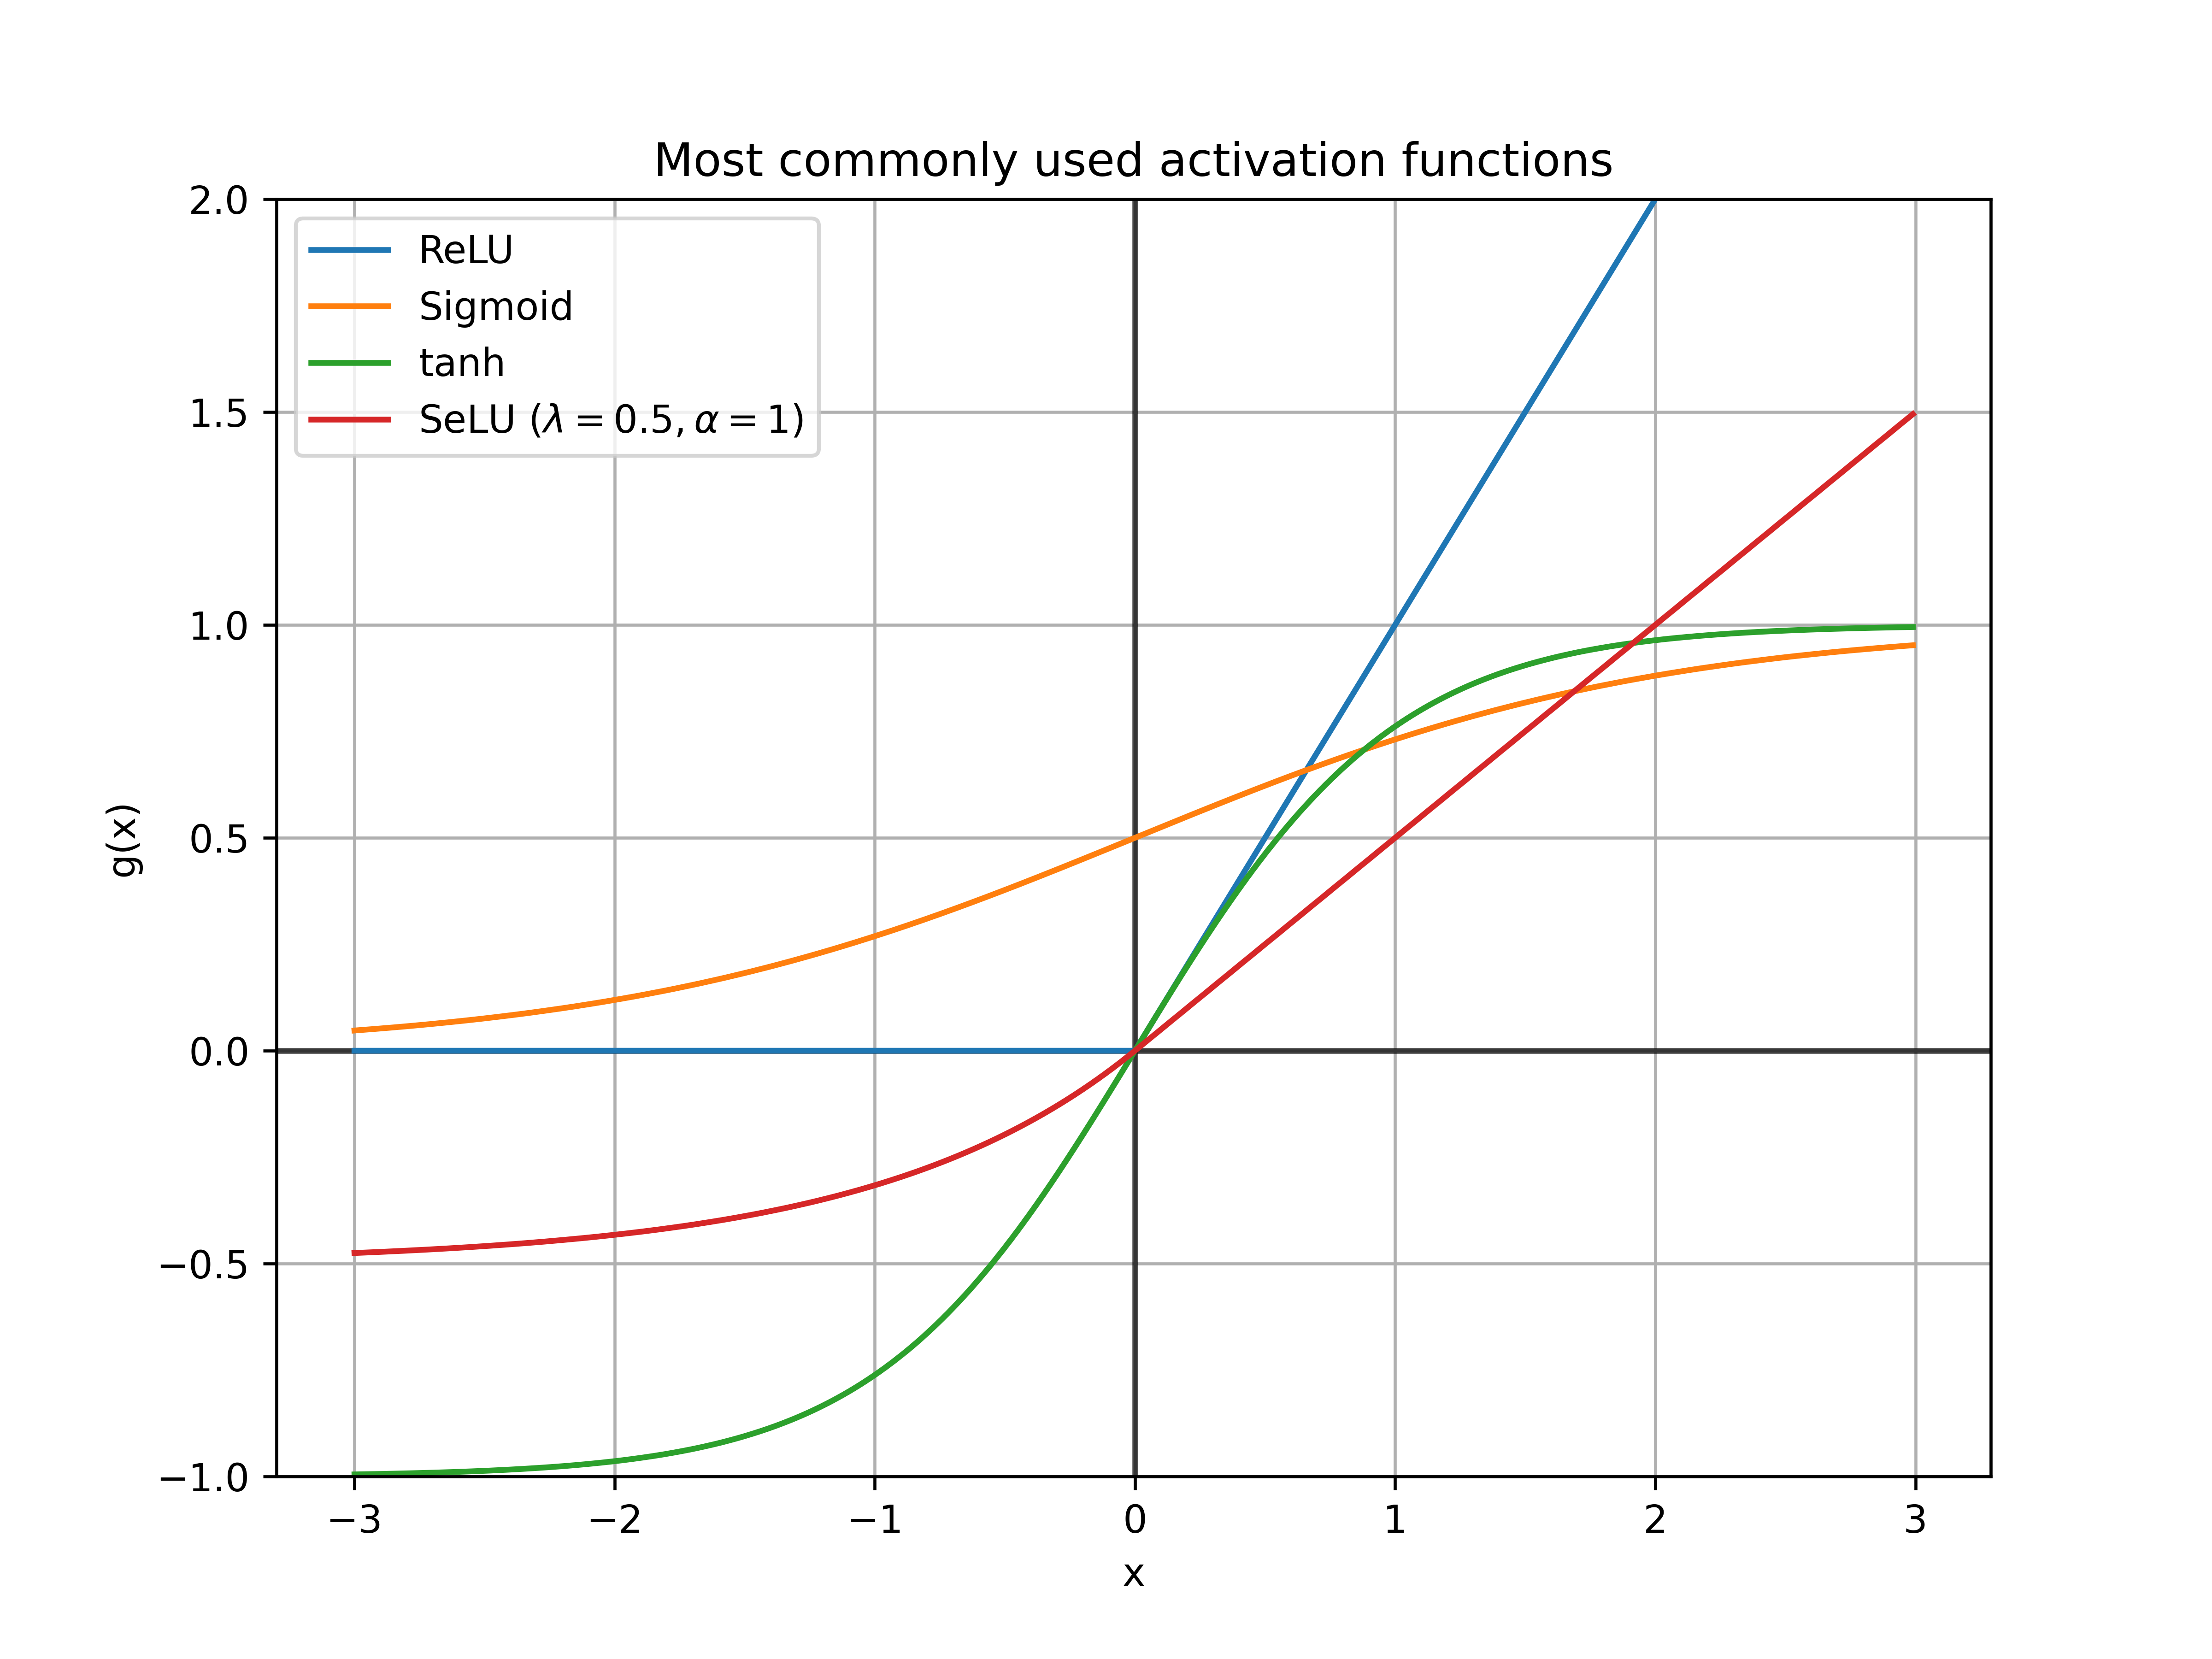
\includegraphics[width=0.7\linewidth]{figures/neural_networks/activations}
	\caption{Most commonly used activation functions. Note the plateaus of the sigmoid and tanh functions and for all $x$<0 for ReLU. Setting the gradient zero in case of ReLU for $x$<0 renders several parameters inactive during training; on the other hand, large positive parameters do not get stuck due to vanishing gradients and the function is scaleless.}
	\label{fig:activations}
\end{figure}

\Subsubsection{Objective Functions}

Having established the network structure, a measure of fit quality remains to be chosen. Such measures are called objective functions (error or loss functions) and used to govern the training by setting the gradients of the trainable parameters $\theta$.
Several loss functions have been established for each NN-specific task to be solved. The mean-squared-error (MSE) has been found useful for regression tasks due to its resemblance to the least-squared-error obtained from likelihood fits of normal distributed data. The so-called cross-entropy error function has been found performant for classification tasks due to the relation of the loss to information theory and the accessible probabilistic interpretation of the outputs following sigmoid activation. Both of these loss functions need target labels to compare the network outputs to. Training procedures where fixed labels guide the parameter estimation are called supervised learning.

Distribution fitting requires the loss function to compare samples from a probability distribution function to a target distribution. Since the discrete labels are replaced with continuous target distributions and none of the datapoints has a well-defined target these training procedures belong to the class of unsupervised learning. As the name suggests, the neural network does not obtain any additional feature representation of the data necessary for the optimization procedure. In layman's terms the network has to "figure out on its own" which input features are more important for the given task.

In this work, distribution fitting will be performed which is reflected by the choice of the loss function. The Kullback-Leibler divergence (also called relative entropy) is a measure of resemblance of $p_\text{x}(x; \theta)$ to $q_\text{x}(x)$, both defined over the random variable \text{x}, and belongs to the families of $f$-divergences defined as

\begin{equation*}
	D_f\left[q_\text{x}(x) \, \, || \, \, p_\text{x}(x; \theta)\right] = \mathbb{E}_{p_\text{x}(x; \theta)}\left[f\left(\frac{q_\text{x}(x)}{p_\text{x}(x; \theta)}\right)\right]
\end{equation*}

with the convex function $f(r) = r\log r$ \cite{Papamakarios_NF}. In its expanded form it can be written as

\begin{equation}
	\begin{aligned}
		\mathbb{KL}\left[q_\text{x}(x) \, \, || \, \, p_\text{x}(x; \theta)\right] &= \mathbb{E}_{q_\text{x}(x)}\left[\frac{\log q_\text{x}(x)}{\log p_x(x; \theta)}\right] \\&= \underbrace{- \mathbb{E}_{q_\text{x}(x)} \left[ \log p_\text{x}(x; \theta)\right]}_{\mathcal{L}(\theta)} + \underbrace{\mathbb{E}_{q_\text{x}(x)}\left[\log q_\text{x}(x)\right]}_{const}
	\end{aligned}
	\label{eq:KL-loss}
\end{equation}

and can be decomposed into a $\theta$-parameter dependent and a $\theta$-independent term\footnote{Note that the Kullback-Leibler divergence is not symmetric in its arguments and swapping $q$ and $p$ does not yield a similar decomposition due to the expectation value taken over the probability density function $p_\text{x}(x; \theta)$. Hence a distinction between the forward and the backward Kullback-Leibler divergence has to be made. In to following, the forward KL-divergence (introduced above) will be used exclusively.}. The KL-divergence has a global minimum of value 0 where both distributions are identical. With this expression, one can approximate an unknown posterior distribution $p(x | y)$ using a model function $p_\theta(x | y)$ (both conditioned on a random variable $y$) by taking the parameter-dependent term $\mathcal{L}(\theta)$ as a basis for the loss function.

Objective functions "guide" only the training, but are not a measure about the quality of the predictions per se. It can occur in terms of the weights, that a given feature of one or several inputs enjoys a higher-than-optimal weight at the cost of generalization (overfitting and overtraining). For this reason, the entries of the weight matrix during gradient descent are penalized with an additional $L^2$ regularization term

\begin{equation}
	L'(\theta) = L(\theta) + \alpha \, ||\theta|| _2^2
\end{equation}

where $\alpha$ is a fixed regularization parameter.

What is missing from a complete training is data the network is trained with respect to and the optimizer looking for an optimum of the loss function.

%With this choice of the loss, one can potentially generate samples from the true posterior distribution at the global optimum of the KL-divergence. In the following, a likelihood-free solution to the posterior inference problem using conditional invertible neural networks will be discussed.

\Subsubsection{Training and Loss Optimization}

The optimization is data-driven. The dataset is split up to two disjoint datasets: a training and a test set. For every iteration a number of samples from the training set are evaluated through the network from which the current network performance can be evaluated. Ideally, finding a local optimum of a one-dimensional function requires a closed form of the function itself with respect to its parameters. Unfortunately, this is usually not the case due to the high-dimensional and nonlinear nature of the optimization problem. For this reason, the weight matrices are adjusted for every node through backpropagation: the gradients for each hyperparameter are calculated from the previous layer and the parameters are updated through gradient descent along the negative of the parameter gradient moving slowing to a locally optimal value. For a simple case, it can be intuitively written with a positive learning rate $\eta$ as

\begin{equation}
	\theta^t = \theta^{t-1}-\eta\left[\frac{\partial \mathcal{L}}{\partial\theta}\right]^{t-1}
	\label{eq:optimization}
\end{equation}

Note that the learning rate is a decisive parameter in the update process; while a too small value of $\eta$ does not improve the loss significantly, a large $\eta$ on the other hand cannot achieve the desired convergence. To speed up the optimization process, this simple idea has been improved further upon and several competing optimizers have emerged. In this work, the quasi-standard Adam optimizer \cite{Adam_paper} has been used. It uses a sophisticated self-tuning learning rate optimization (taking the "momentum of convergence" into consideration) and several, empirically useful parameters to optimize the convergence. The algorithm can be summarized as the following:

\begin{equation*}
	\begin{cases}
			\theta^{t+1} &= \theta^t - \eta \cdot \frac{\hat{m}^t}{\sqrt{\hat{v}^t}+\epsilon}\\
			g^t &=\nabla_\theta f^t (\theta^{t-1})\\
			m^t&=\beta_1 \cdot m^{t-1} + (1-\beta_1) \cdot g^t \\
			v^t&=\beta_2 \cdot v^{t-1} + (1-\beta_2) \cdot g^t \\
			\hat{m}^t&=\frac{m^t}{1-\beta^t_1}\\
			\hat{v}^t&=\frac{v^t}{1-\beta^t_2}
	\end{cases}
\end{equation*}

Note that while Adam evaluates the next step using multiple measures in a sophisticated manner, in its core and using the right parameters the same gradient descent from eq. \ref{eq:optimization} can be found. It has been found experimentally that the parameters $\beta_1 = 0.9$ and $\beta_2 = 0.999$ are suitable choices for general tasks.

In order to further improve the optimization, the updates are evaluated for a fixed number of samples (batches) which introduces a stochastic nature to it averaging the gradient for the selected samples. The main advantage of stochastic gradient descent is the consecutive updates towards a more general optimum and avoiding getting stuck at local optima due to strongly varying gradients evaluated from the dataset.
Once the whole training dataset has been used up, an epoch has reached its end and the process starts anew with a shuffled training dataset. After several epochs, the procedure converges.
In order to monitor the network performance and its generalization capabilities, the test set is used. For this, the loss can be evaluated for these "unseen" datasamples, which can show signs of anomalies during training. Should for example the test loss rise while the training loss decreases, one can be certain that overtraining has had occurred.

\Subsection{Conditional Invertible Neural Networks}

Conditional Invertible Neural Networks have been found performant in machine learning tasks such as image colouring and guided image generation with style transfer \cite{cINN_im_gen}, parton shower generations and detector effect simulation \cite{Bellagente_2020}, stellar parameter determination \cite{Ksoll_2020} and cosmic ray source property inference \cite{Bister_2022}.

Most neural network setups tackle the challenge of posterior inference where the probability distribution 

\begin{equation*}
	p(x | y) = \frac{p(y | x) p(x)}{p(y)}
\end{equation*}

in Bayes' Theorem cannot be evaluated analytically. Most of these models are constructed in a one-directional way and do not preserve probability during inference. For this reason, even for (potentially) invertible problems, the model inverse is ill-defined. To avoid this, the network architecture has to be adjusted to satisfy the requirements of invertibility.

\Subsubsection{General INN Architecture}

To ensure invertibility the network input and output dimensions have to match to fulfil bijection. General invertible neural networks map the inputs $x$ to their targets $y$ while encoding some information regarding $x$ in the latent variables $z$. These variables are assumed to follow a fixed distribution which is also represented in the loss function. Usually these distributions are chosen to be a multivariate normal distribution, as they are unbiased and easy to sample from, the latter being crucial for obtaining the posterior distributions $p(x | y)$. Indeed, it can be shown that upon perfect convergence sampling from the latent space and picking an $y$ network inference yields the true posteriors $p(x | y)$ for any $y$ \cite{INN_Ardizzone}.

\begin{figure}[h!]
	\centering
	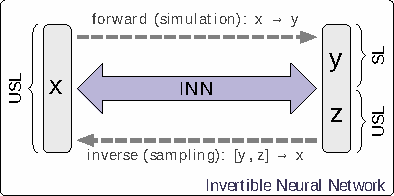
\includegraphics[width=0.6\linewidth]{figures/neural_networks/inns.pdf}
	\caption{General INN structure. Uniquely to these structures\protect\footnotemark, the network can be trained in both directions with a supervised loss (SL) term for the target labels $y$ and an unsupervised loss term (USL) for the latents $z$ and inputs $x$. \cite{INN_Ardizzone}}
	\label{fig:inn}
\end{figure}

\footnotetext{but not for cINNs}

A conceptual disadvantage arises from the conditions being included in the network outputs. Assuming the dimensionality of $x$ and $y$ are wide apart from each other zero-padding or several noise-extending techniques are necessary to construct the network potentially introducing unnecessary redundancies. This can be fixed by removing the conditions $y$ from the output and by using them as an additional input for the network and by setting the dimension of the latent space distribution to match that of the inputs $x$. With this approach, the conditions can also be pre-processed by applying a -- either pre- or jointly with the network trained -- network (a conditioning or summary network) \cite{BayesFlow}. Such setups enable processing of highly correlated or feature-rich data at the cost of potential overfitting \cite{Ksoll_2020}. 
%A sketch of the resulting network -- the conditional invertible neural network (cINN) -- structure is shown in fig. \ref{fig:cINN_archicture}.

%\begin{figure}[h!]
%	\centering
%	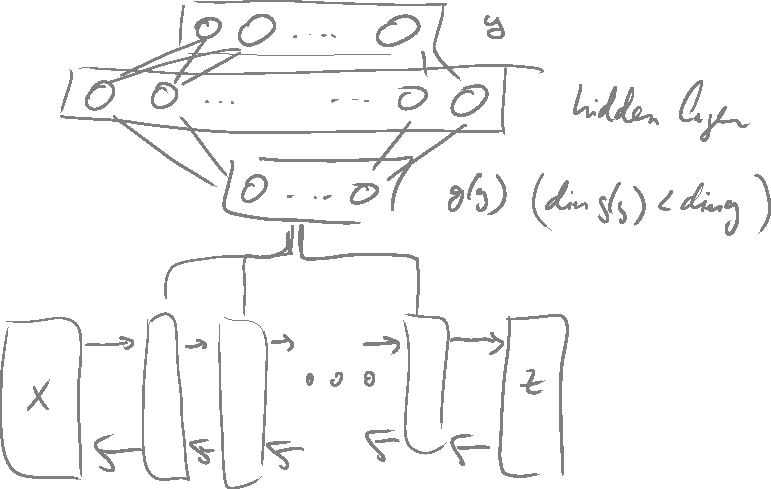
\includegraphics[width=0.4\linewidth]{figures/neural_networks/SN-cINN.pdf}
%	\caption{\textcolor{red}{A sketch of the network setup with a summary network}}
%	\label{fig:cINN_archicture}
%\end{figure}

By constructing an invertible structure, the challenge of exact posterior inference remains with the added difficulty of mapping the inputs to the latent space distribution (LSD) in a meaningful (invertible and information conserving) way. To tackle this challenge, normalizing flows (NF) have to be applied.

\Subsubsection{Normalizing Flows}

The main idea of NFs is to construct an invertible transformation $T$ which maps a probability distribution $p$ to a target probability distribution $q$ in an invertible way. Hence, both $T$ and its inverse $T^{-1}$ have to be invertible and differentiable to preserve the probability flow. Such mappings are called diffeormophisms; note that a composition of diffeomorphisms

\begin{equation*}
	T' = T_1 \circ T_2 \circ ... \circ T_N
\end{equation*}

yields a diffeomorphism too.

In a historic sense a whitening transformation can be already viewed as a normalizing flow the target distribution being a (multivariate) normal distribution. In more general and complicated cases however, the transformation $T$ cannot be easily constructed by hand. As the transformation is applied to samples of the distribution $p$, the flow has to normalize the distribution internally.

Assume we would like to express the probability $p(x)$ using the target distribution. For this, a straightforward coordinate transformation involving the Jacobian from the source to the target space can be used:

\begin{equation*}
	p(x) = p(z) \left| \det J_T \right| = p(z) \left| \frac{\partial x}{\partial z} \right|
\end{equation*}

The backward transformation can be written using the inverse of $T$ and its determinant

\begin{equation*}
	p(z) = p(x) \left| \det J_{T^{-1}} \right| = p(x) \left| \frac{\partial z}{\partial x} \right|
\end{equation*}

Here we can directly observe the explicit reason why $T$ has to be diffeomorphism. A graphical representation of a normalizing flow for two-dimensional distributions can be seen in fig. \ref{fig:NF_example}.

\begin{figure}[h!]
	\centering
	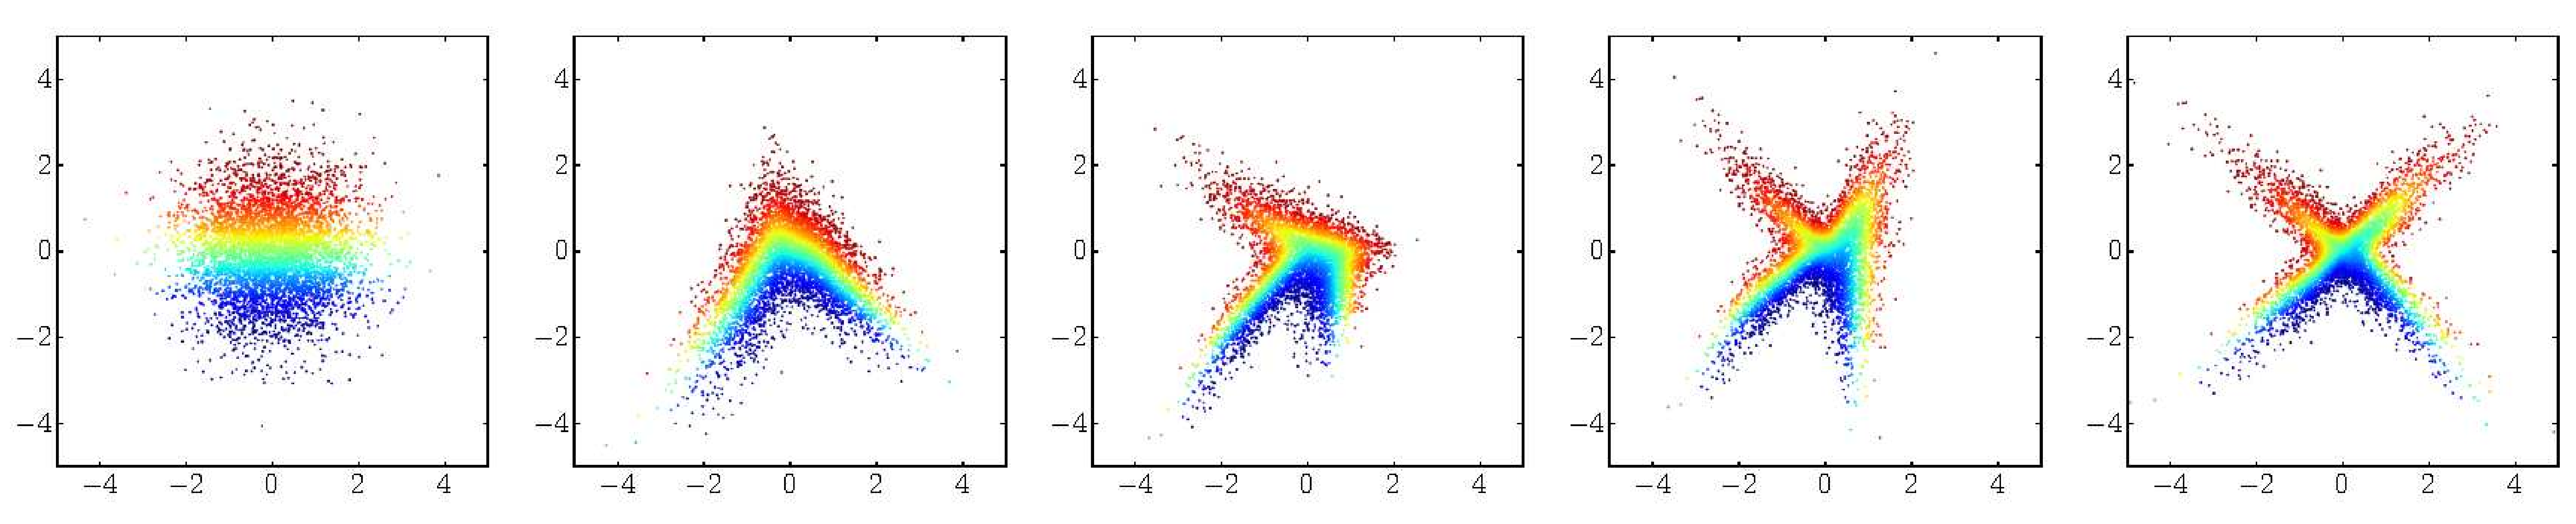
\includegraphics[width=\textwidth]{figures/neural_networks/flow}
	\caption{Example of a normalizing flow transforming a normal distribution to a star-shaped one in 4 steps. Note that the subsequent steps are also done with diffeomorphisms while the resulting transformation still remains a diffeomorphism. \cite{Papamakarios_NF}}
	\label{fig:NF_example}
\end{figure}

cINNs use neural networks to learn the mapping $T$. In the following, the construction of the diffeomorphic transformation will be discussed in detail.

\Subsubsection{Affine Coupling Blocks}

To represent the transformation $T$ Affine Coupling Blocks (ACB) can be utilized. In this work, exclusively the Generative Flow (GLOW) coupling block \cite{glow_paper} will be used. The GLOW block follows a design similar to the RealNVP block from \cite{RealNVP}. These blocks in practice need to fulfil at least two conditions: first, they have to invertible and second, the Jacobian of the mapping it represents has to be numerically tractable, especially its determinant. The GLOW block fulfils both of these conditions. In order to do so, it first splits up its input $u = [u_1, u_2]$ in two equal parts, on which a scaling $s_i(\cdot)$ and a translation $t_i(\cdot)$ using arbitrary, non-invertible functions are applied. The resulting transformation reads

\begin{equation}
	\left\{\begin{aligned}
		v_1 &= u_1 \odot \exp(s_2(u_2)) + t_2(u_2) \\
		v_2 &= u_2 \odot \exp(s_1(v_1)) + t_1(v_1)
	\end{aligned}\right.
	\label{eq:glow_transformation}
\end{equation}

where $\odot$ denotes the element-wise (Hadamard) product. Note that although the functions $s_i(\cdot)$ and $t_i(\cdot)$ are not necessary invertible themselves and can be approximated thanks to the Universal Approximation Theorem with neural networks, the transformation in eq. \ref{eq:glow_transformation} is invertible, as $u_1$ and $u_2$ can be expressed with $v_1$ and $v_2$:

\begin{equation*}
	\left\{\begin{aligned}
		u_1 &= (v_2 - t_1(v_1)) \odot \exp(-s_1(v_1)) \\
		u_2 &= (v_1 - t_2(u_2)) \odot \exp(-s_2(u_2)) 
	\end{aligned}\right.
\end{equation*}

At this point, the exponential functions may seem arbitrary. Looking at the Jacobian

\begin{equation*}
	\frac{\partial (v_1, v_2)}{\partial(u_1, u_2)} = \left(\begin{matrix}
		\exp(s_2(u_2)) & \frac{\partial v_1}{\partial u_2} \\
		0             & \exp(s_1(v_1))
	\end{matrix}\right)
\end{equation*}

and its determinant

\begin{equation*}
	\left|\frac{\partial (v_1, v_2)}{\partial (u_1, u_2)} \right| = \exp \left(\sum_j s^j_2(u_2) + s^j_2(v_1) \right)
\end{equation*}

it can be seen that they keep the determinant is nonzero independently of the behaviour of the scaling transformations $s_i(\cdot)$. It becomes also clear from the determinant, that even for high-dimensional input and output vectors $u$, $v$ the determinant is computationally cheap to evaluate.

Due to their mutual dependence on each other the expressions in eq. \ref{eq:glow_transformation} are not evaluated directly in practice and the transformation is split up in two intermediate steps. First, a term with

\begin{equation*}
	f_1(u_1, u_2) = (v_1, u_2) = \begin{cases}
		u_1 \odot \exp(s_2(u_2)) + t_2(u_2) \\
		u_2
	\end{cases}
\end{equation*}

is evaluated followed by

\begin{equation*}
	f_2(v_1, u_2) = (v_1, v_2) = \begin{cases}
		v_1 \\
		 u_2 \odot \exp(s_1(v_1)) + t_1(v_1)
	\end{cases}
\end{equation*}

It is easy to check, that the composed transformation $f = f_2 \circ f_1$ has the same Jacobian (and hence the same determinant) as the one in eq. \ref{eq:glow_transformation}. This step-wise evaluation can be visualized in a flow chart, as shown in fig. \ref{fig:glow}.

\begin{figure}[h!]
	\centering
	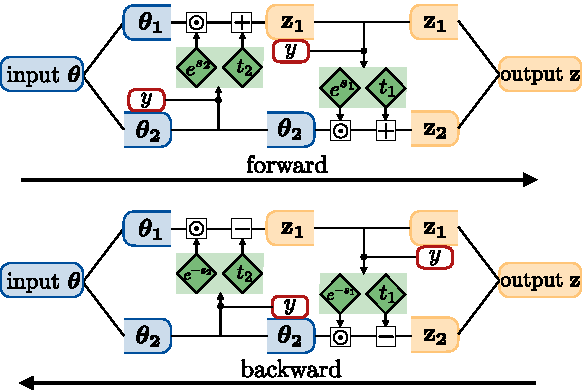
\includegraphics[width=\linewidth]{figures/neural_networks/glow.pdf}
	\caption{The forward and the backward pass of the GLOW block. Note that per construction, the sub-networks do not have to invertible themselves, and the block can be evaluated in both directions. The conditions node $c$ is used as an additional input for each sub-network. \cite{Ksoll_2020}}
	\label{fig:glow}
\end{figure}

Note that the exponential functions in eq. \ref{eq:glow_transformation} can potentially produce extreme values which can lead to numerical instabilities during optimization. For this reason, additional soft-clamping is introduced, and an additional scale function with a fixed clamping coefficient $\alpha$ is applied to the scale coefficients $s_i(\cdot)$:

\begin{equation*}
	s' = \frac{2\alpha}{\pi} \arctan\left(\frac{s}{\alpha}\right)
\end{equation*}

For $\lim\limits_{s\rightarrow\pm\infty} s' = \alpha$, while $s' \approx s$ if $s$ is of the same order of magnitude as $\alpha$. This naturally dampens the gradients from one block to the other meaning $\alpha$ has to be carefully chosen to avoid information loss between the consecutive blocks. For most analyses clamping coefficients of $\alpha \approx 1.9$ suffices.

With the construction of the normalizing flow with the GLOW block and the subnetworks representing the scaling $s_i(\cdot)$ and transitions $t_i(\cdot)$, the setting of the loss function using the Kullback-Leibler divergence remains to construct the whole cINN.

\Subsubsection{The Kullback-Leibler Divergence as a Loss Function}

Our goal is to approximate the real posterior distribution of a physics parameter $x$ under the observation $y$, i.e. we would like to write:

\begin{equation*}
	p(x | y) \approx p_\theta(x | y)
\end{equation*}

With the Kullback-Leibler divergence from eq. \ref{eq:KL-loss}, this can be formalized with $q(x) = p(x | y)$ and $p(x; \theta) = p_\theta(x | y)$ as

\begin{equation*}
	\mathbb{KL}\left[p(x | y) || p_\theta(x | y) \right] = - \mathbb{E}_{p(x | y)} \left[ \log p_\theta(x | y)\right] + const.
\end{equation*}

This form of the KL-divergence can be understood in terms of likelihoods as finding the optimal parameters which maximize the likelihood is asymptotically equivalent to finding the distribution which has minimal distance to the real distribution in terms of the KL-divergence \cite{Bishop_book}. This expression can now be rewritten using the Jacobian and the known and fixed latent space distribution as

\begin{equation*}
	\begin{aligned}
		\mathbb{KL}\left[p(x | y) || p_\theta(x | y) \right] &= - \mathbb{E}_{p(x | y)}\left(\log p(z) \left|\det\frac{\partial z}{\partial x}\right|\right) + const. \\
		&= - \mathbb{E}_{p(x | y)}\left(\log p(z)  + \log \left|\det\frac{\partial z}{\partial x}\right|\right) + const.
	\end{aligned}
\end{equation*}

where $z = f(x, y, \theta)$ is the output of the network in the latent space. At this point we can fix the distribution $p(z)$ to be a multivariate Gaussian of mean 0 and standard deviation 1. Writing

\begin{equation*}
	p(z) \propto \mathcal{N}(z; \mu = 0, \Sigma=\mathbb{1}) \propto \exp\left(-\frac{z^2}{2}\right)
\end{equation*}

the resulting loss function becomes

\begin{equation*}
	\mathcal{L}(\theta) = \frac{1}{M} \sum_{m=1}^{M} \frac{f(x_m; \theta)^2}{2} - \log\left|\det\frac{\partial f(x_m; \theta)}{\partial x}\right|
\end{equation*}

for all inputs $x_m$ of batch $m$ to train the network with respect to.

\Subsubsection{Posterior Inference}
After training, the network should be capable of inferring the true posterior distribution. For this, a condition has to be fixed first. Then, one can select samples from the latent space distribution (as its shape has been fixed by the loss function) and invert the network to obtain the samples from the posterior distribution.
At first glance there is no guarantee from the loss and from the architecture only that it is meaningful to map the datapoints to a more or less arbitrary function, from which independently drawn samples can be used for posterior inference. However, it can be shown that the latent output distribution is statistically independent on the training data at the global optimum, and the latent output distribution is the same for any fixed condition \cite{BayesFlow}. This motivates the rightfulness of the sampling from the latent space.



% analysis
\pageshift
\thispagestyle{plain}
\Section{Analysis- Strategy and Setup}
\label{ch:analysis_strategy}

In this chapter, an overview of the analysis- strategy and setup will be given with a special focus on the physical observable used as the condition for the cINN inference.

\Subsection{Analysis Strategy}

The analysis has been performed on Monte Carlo (MC) simulated events exclusively. The datasets used for the analysis have been simulated with \texttt{PYTHIA} \cite{Sj_strand_2008} and \texttt{HERWIG++} \cite{herwig}. These simulated events do not only contain matrix element calculation and hadronization, but also the CMS detector simulations using \texttt{GEANT4} in order to represent the final expected distributions accurately \cite{geant1, geant2, geant3}.
The signal processes are \texttt{ggZH} (for the box and triangle diagram process), \texttt{ZH\_DY} (for the Drell-Yan-like $ZH$ production process) and \texttt{WH} (for the $WH$ Higgsstrahlung process). The list of the signal sample datasets is shown in tab. \ref{tab:signal_datasets}. The phase space has been selected to contain regions with high signal sensitivity. Hence the $qq \rightarrow WH \rightarrow b\bar{b} l\nu_l$ and $gg/qq \rightarrow ZH \rightarrow b\bar{b}l\bar{l}$ final states have been considered. The Feynman diagram of these processes are shown in fig. \ref{fig:VH_finalstates}. Note that due to their weakly-interacting nature, neutrinos cannot be reconstructed in the detector. For this reason, former will be referred to as one-lepton and the latter as two-lepton final state with lepton meaning electrons or muons exclusively.

\begin{table}[h!]
	\centering
%	\includegraphics[width=\linewidth]{imagefile}
	\begin{tabular}{c|c}
		Gluon Fusion & Quark Initiated \\
		\hline
		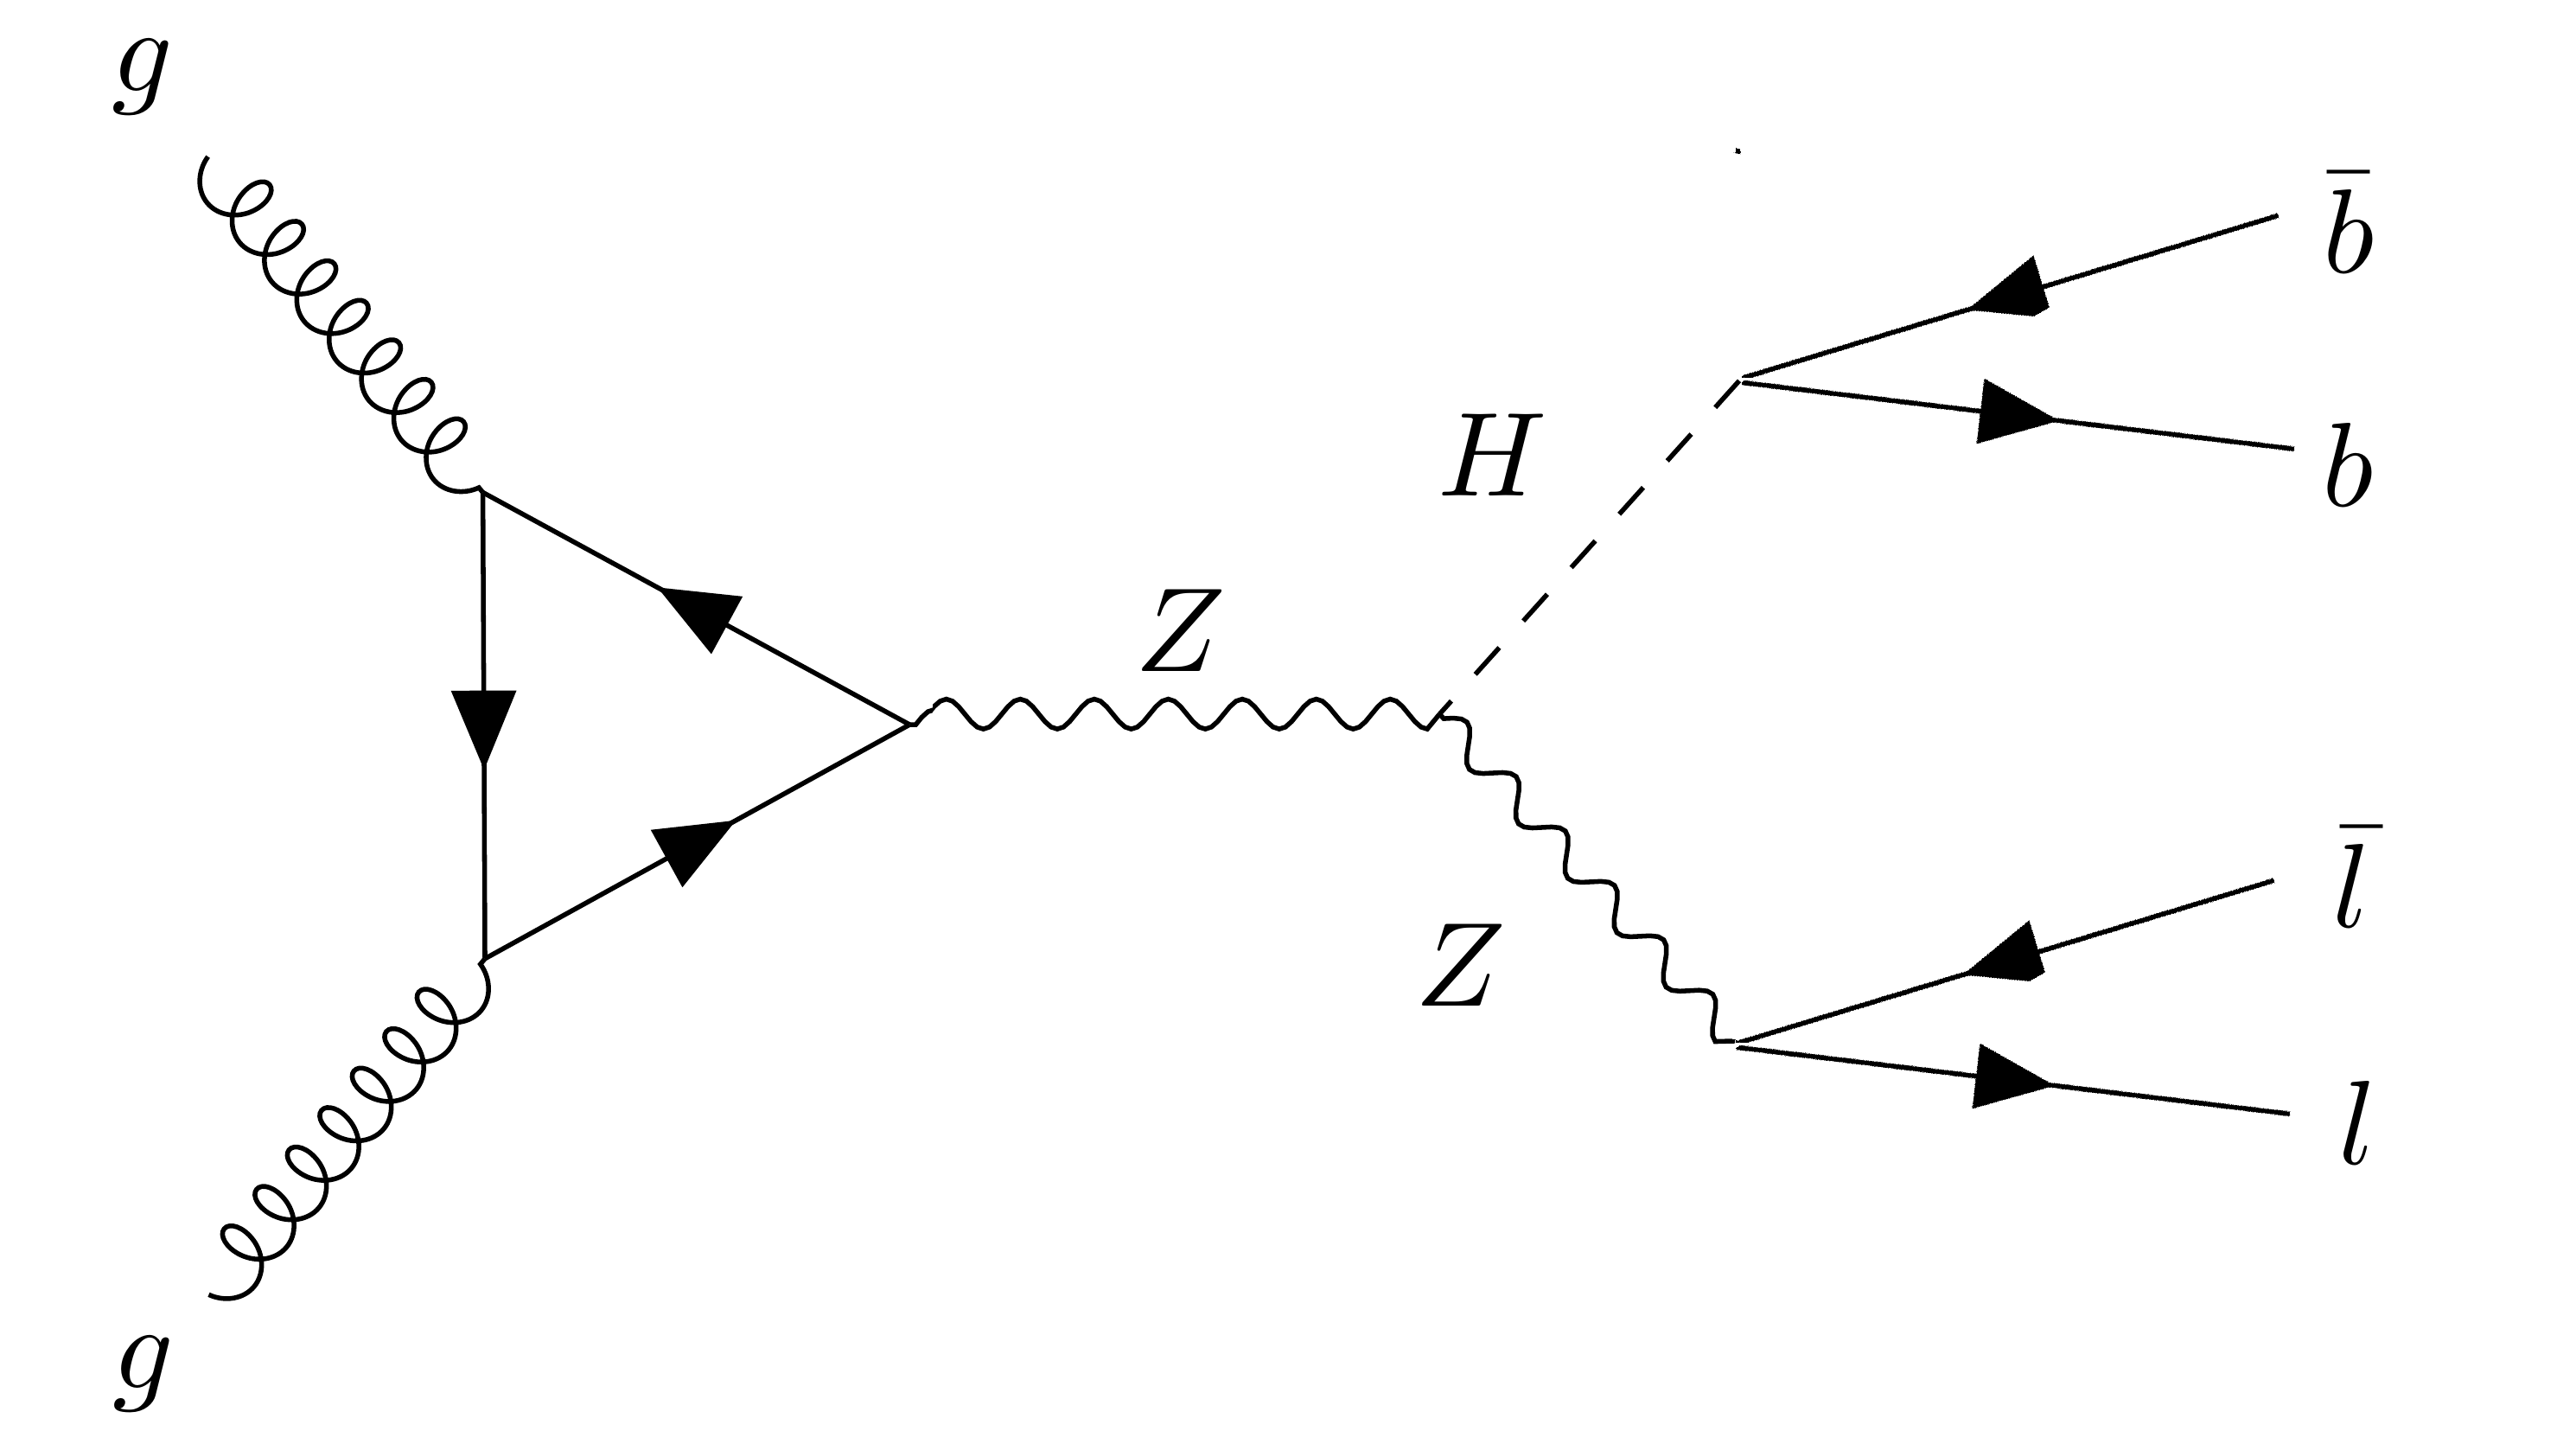
\includegraphics[width=0.4\linewidth]{figures/analysis/ggZH_triangle_bbll}&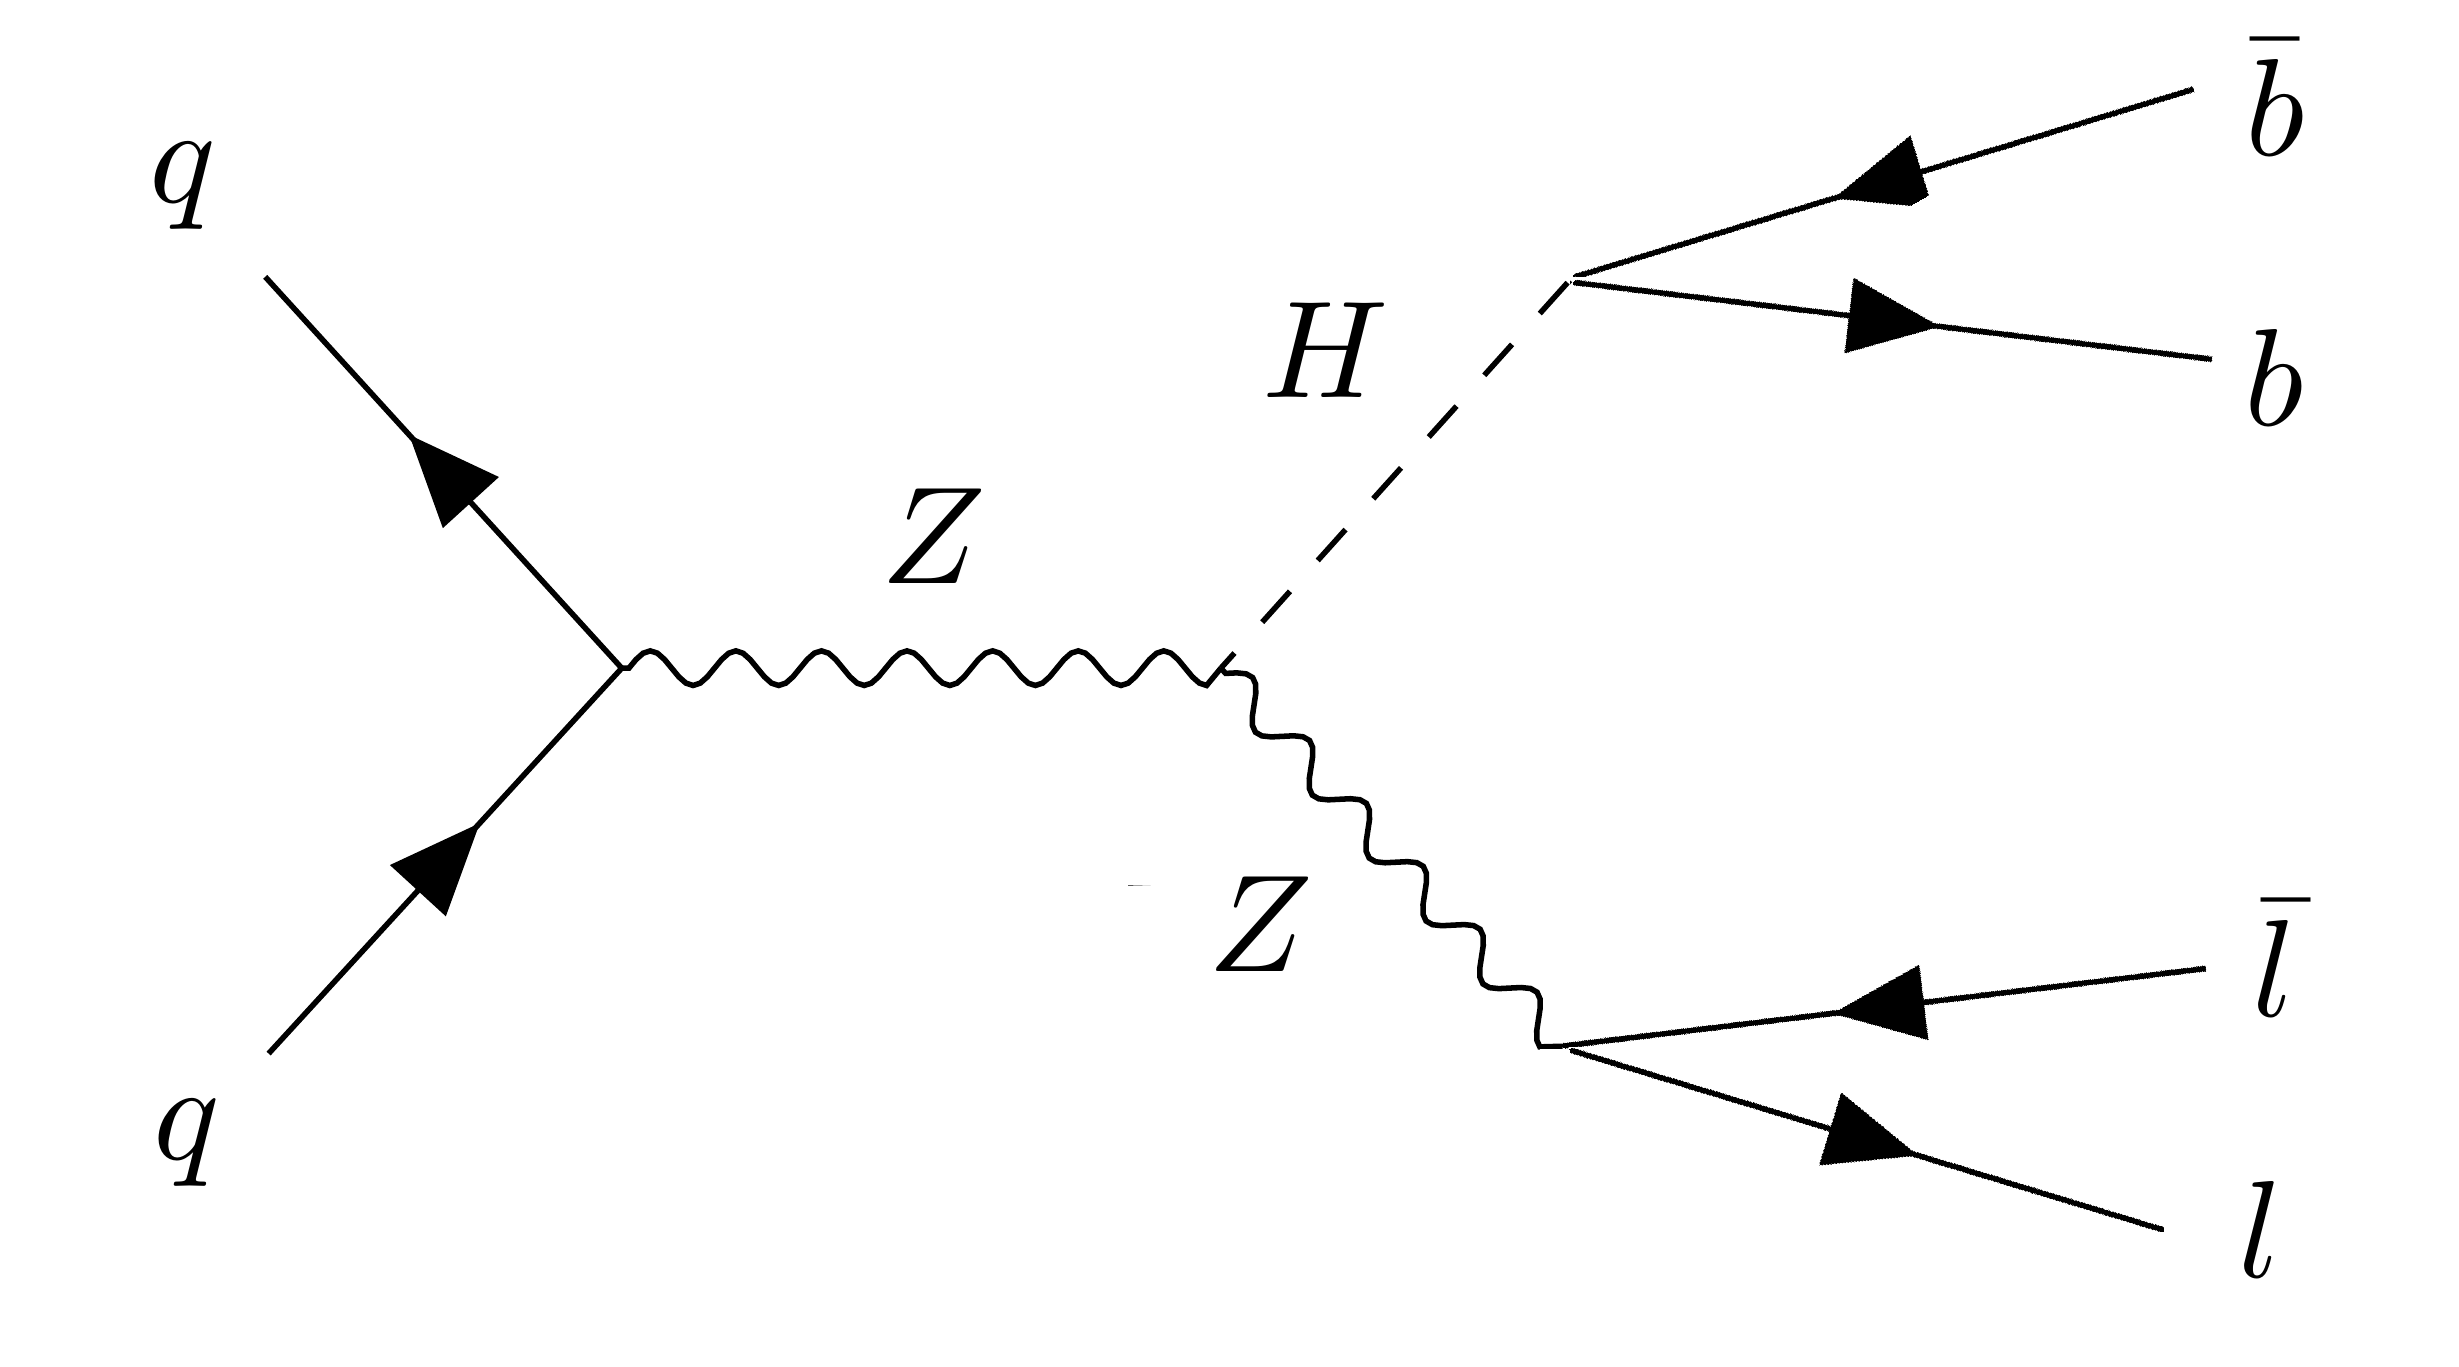
\includegraphics[width=0.4\linewidth]{figures/analysis/ZH_DY_bbll}  \\
		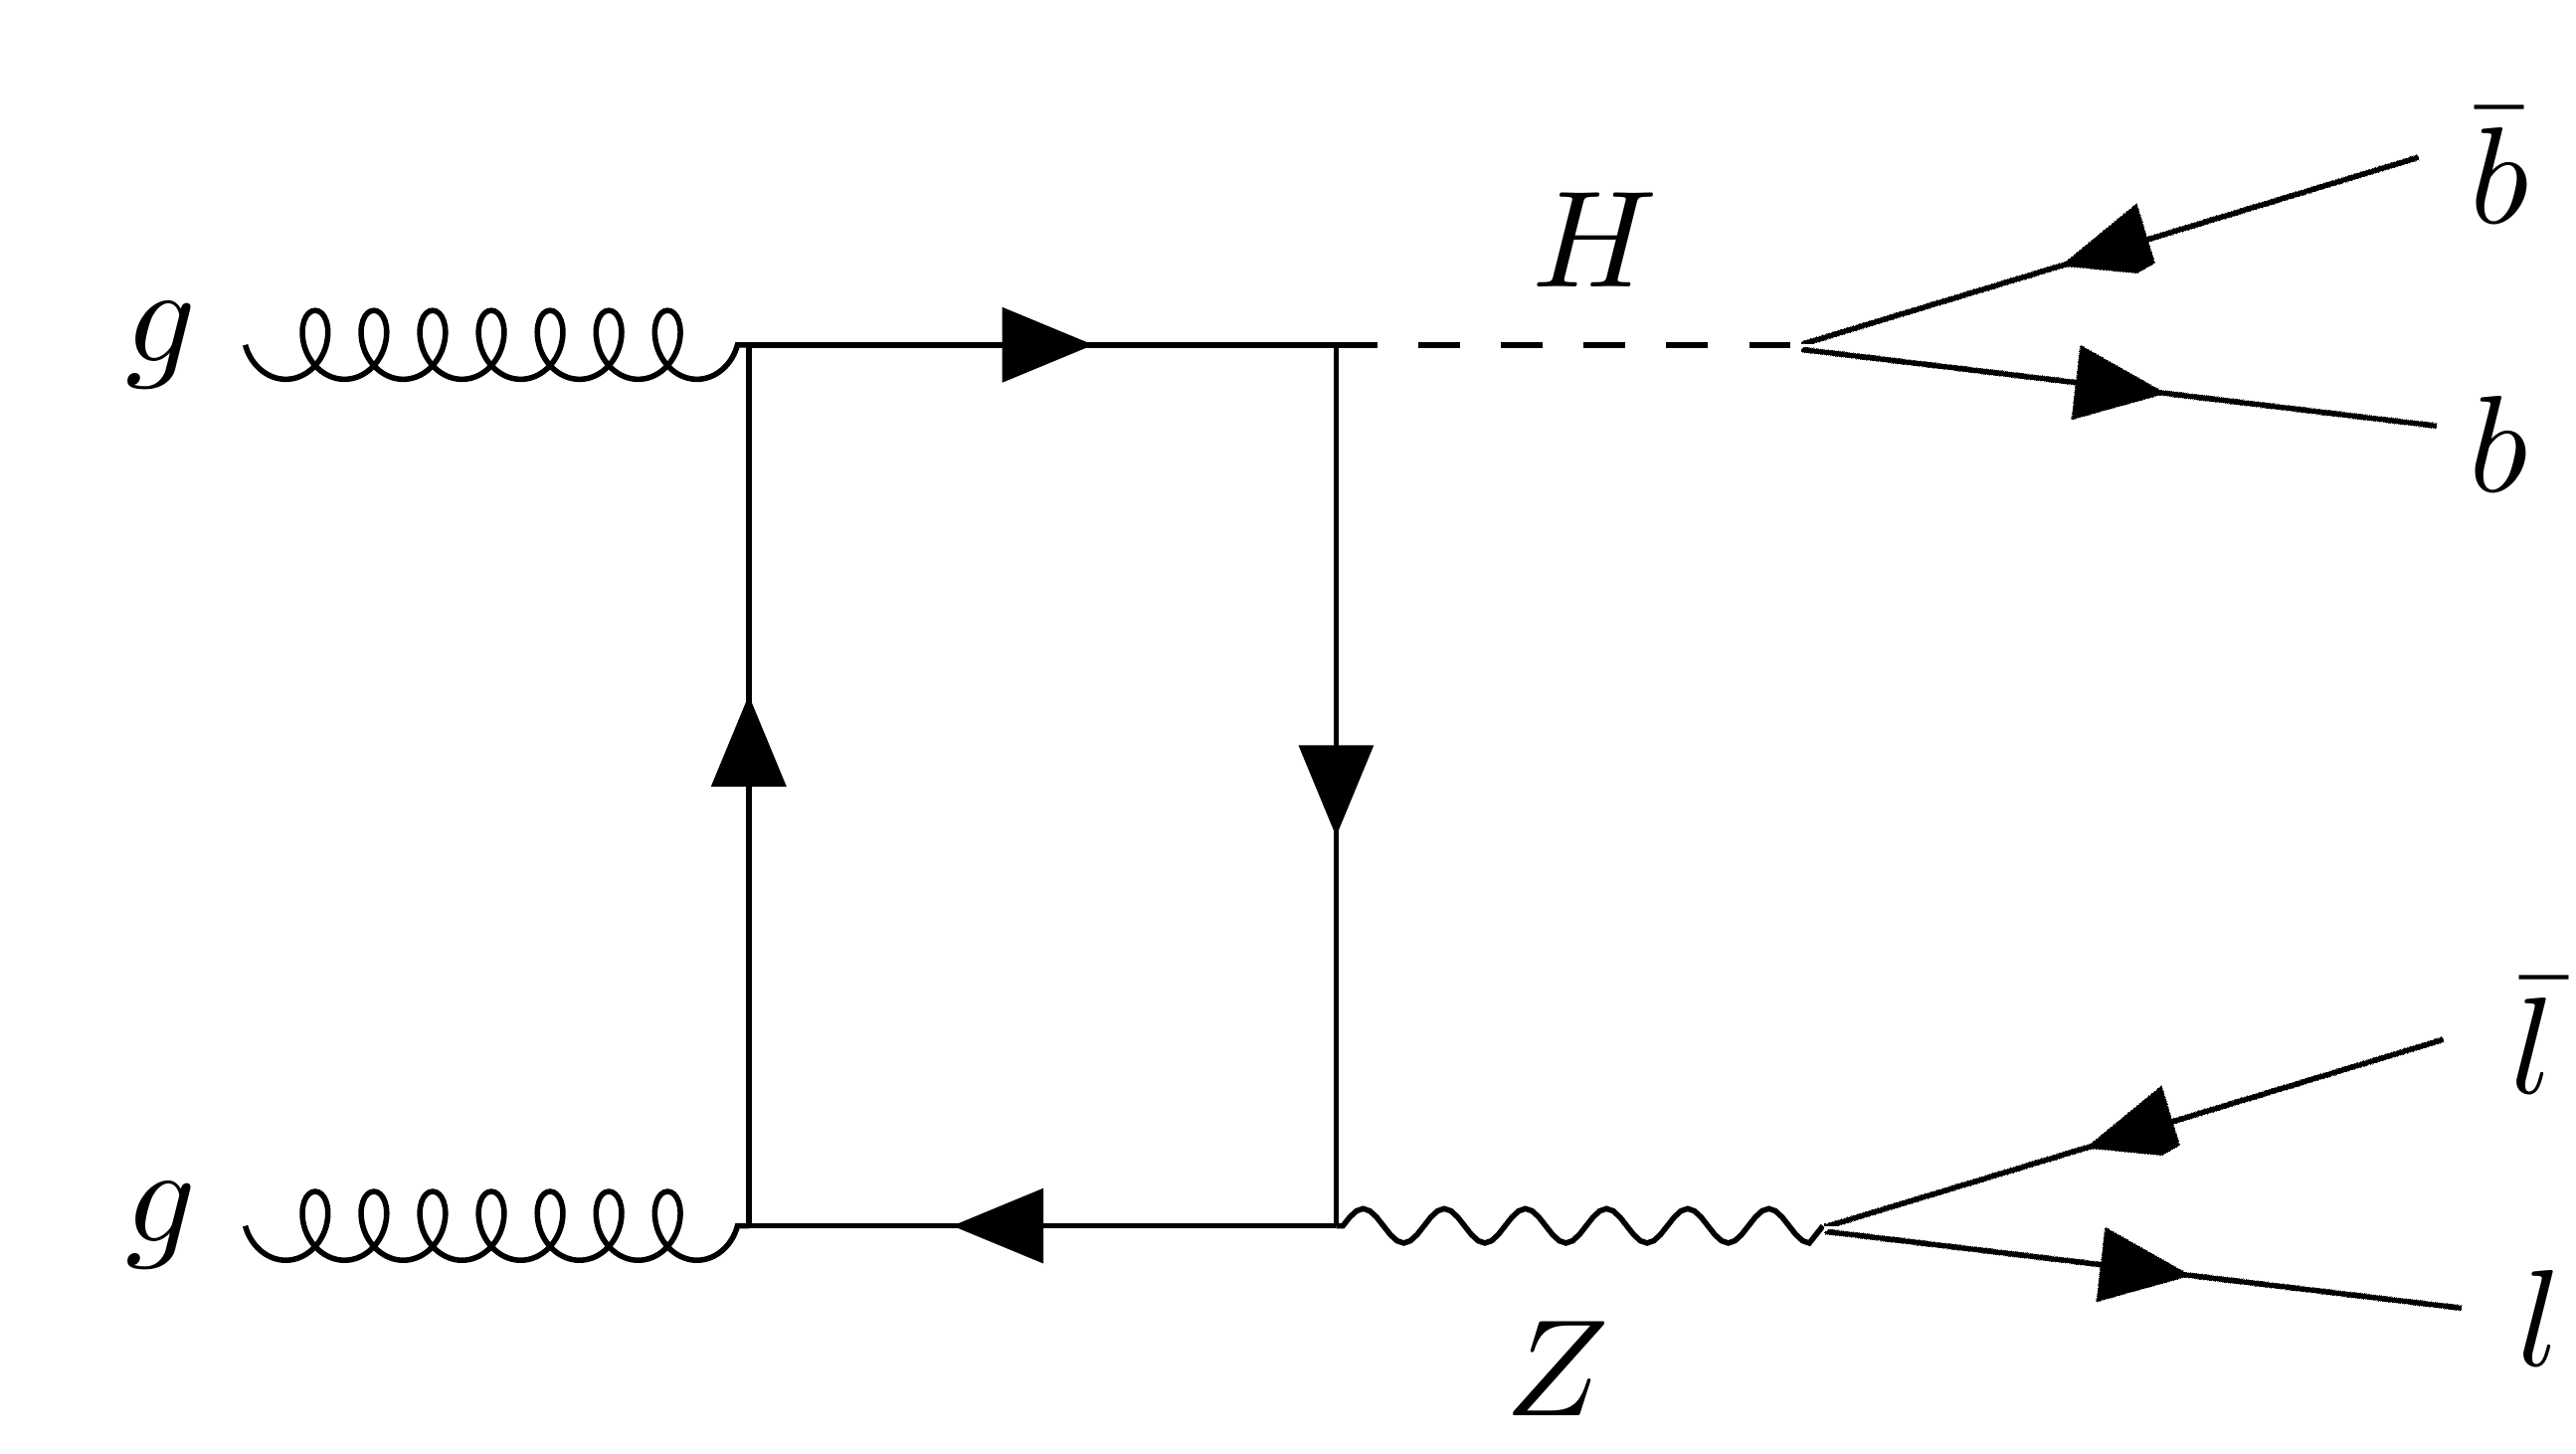
\includegraphics[width=0.4\linewidth]{figures/analysis/ggZH_box_bbll}& 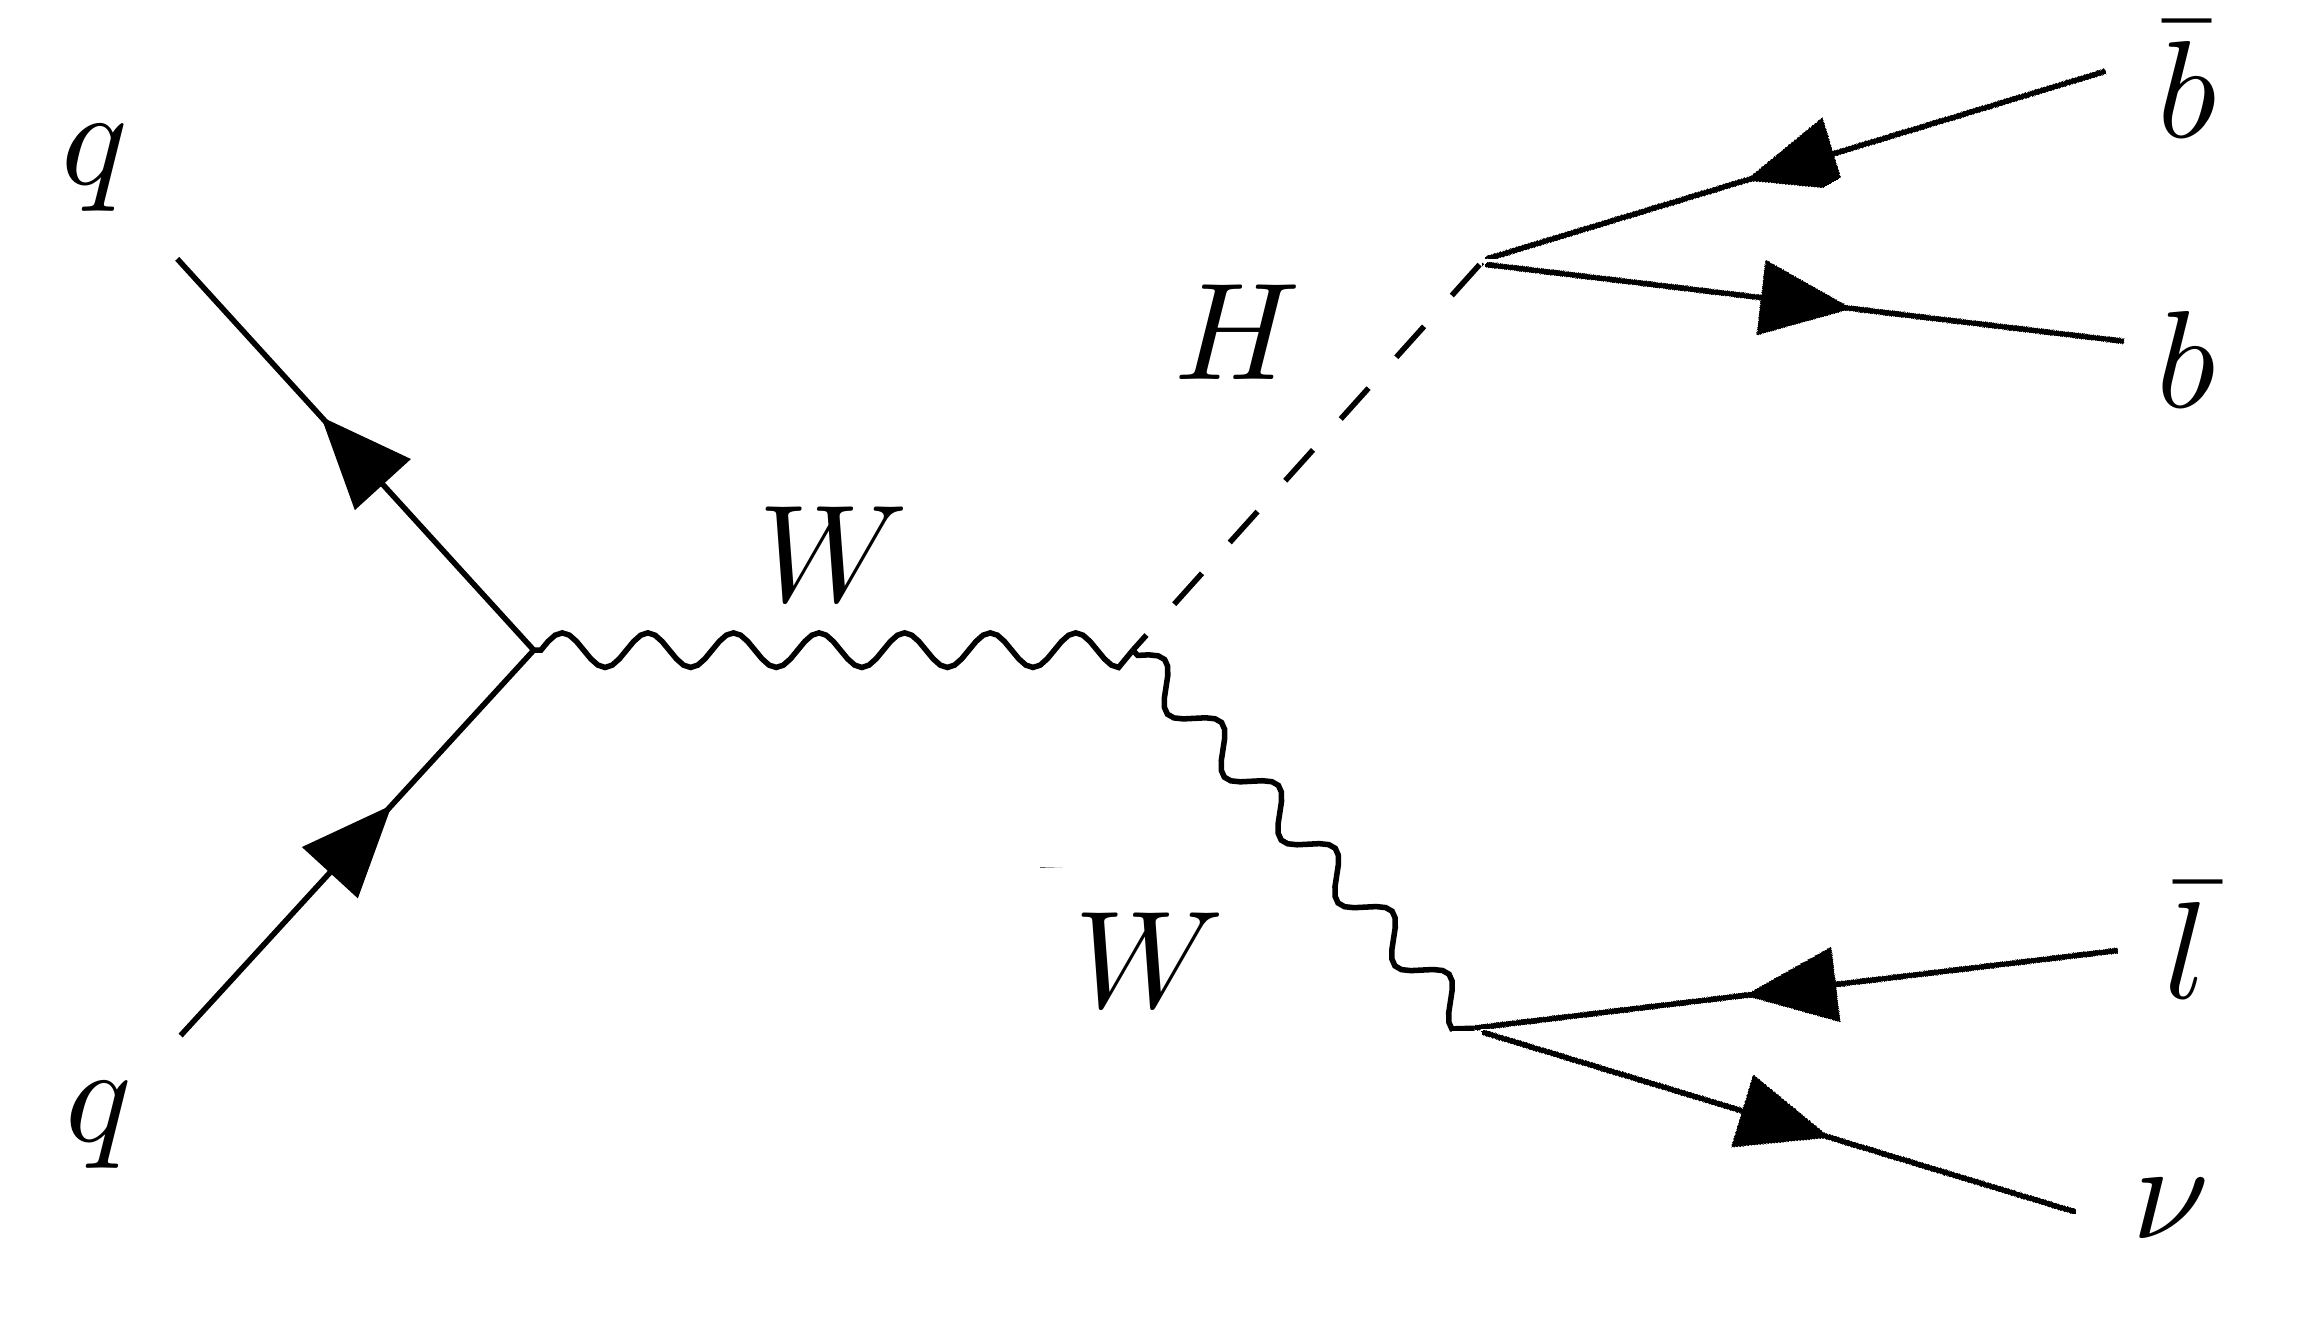
\includegraphics[width=0.4\linewidth]{figures/analysis/HWbbl} \\
	\end{tabular}
	\caption{The analysed final states of the $VH$ processes.}
	\label{fig:VH_finalstates}
\end{table}

The events are categorized through a triggering system and are assigned to one of four channels. The list of the triggers for the two and one lepton channels are listed in tab. \ref{tab:triggers}.

\begin{table}[h!]
	\centering
	\begin{tabular}{cc}
		Channel & Trigger Name \\
		\hline 
		\multirow{2}{*}{$ee$} & \texttt{Ele23\_Ele12\_CaloIdL\_TrackIdL\_IsoVL} \\
		& \texttt{Ele23\_Ele12\_CaloIdL\_TrackIdL\_IsoVL\_DZ} \\
		\hline 
		\multirow{2}{*}{$e$} & \texttt{Ele32\_WPTight\_Gsf} \\
		& \texttt{Ele32\_WPTight\_Gsf\_L1DoubleEG} \\
		\hline 
		\multirow{2}{*}{$\mu\mu$} & \texttt{Mu17\_TrkIsoVVL\_Mu8\_TrkIsoVVL\_DZ} \\
		& \texttt{Mu17\_TrkIsoVVL\_Mu8\_TrkIsoVVL\_DZ\_Mass3p8} \\
		\hline 
		\multirow{2}{*}{$\mu$} & \texttt{IsoMu24\_eta2p1} \\
		& \texttt{IsoMu27} \\
		\hline \\
	\end{tabular}
	\caption{The lepton triggers used in the analysis. For a channel, only one of the given two is used.}
	\label{tab:triggers}
\end{table}

The naming in tab. \ref{tab:triggers} indicates the phase space which the triggers select. In the two lepton channels the lepton with the higher transverse momentum (the leading lepton) is required to have $p_T > \SI{23}{\giga\electronvolt}$ and $p_T > \SI{17}{\giga\electronvolt}$ for $ee$ and $\mu\mu$, respectively; the sub-leading lepton is then required to have $p_T>\SI{12}{\giga\electronvolt}$ and $\SI{8}{\giga\electronvolt}$ for $ee$ and $\mu\mu$, respectively. In the one lepton categories, only electrons with $p_T>\SI{32}{\giga\electronvolt}$ and isolated muons with $\SI{24}{\giga\electronvolt}$ and $|\eta|<2.1$ or isolated muons with $p_T>\SI{27}{\giga\electronvolt}$ are kept.

%In addition to these selection criteria, both muon tracks have to be isolated in the $\mu\mu$ channel. For the $e$ channel, the tight working point has been selected as trigger efficiency.

\begin{table}[h!]
	\centering
	\begin{tabular}{lS[table-format=8.0]S[table-format=1.6]}
%		\toprule
		Dataset name&{N}&$\sigma/$\si{\pico\barn} \\
		\midrule
		\verb|ZH_HToBB_ZToLL_M125_13TeV_powheg_pythia8|&9530684 &0.04471\\
		\verb|ggZH_HToBB_ZToLL_M125_13TeV_powheg_herwigpp|& 199131&0.00722\\
		\midrule
		\verb|WminusH_HToBB_WToLNu_M125_13TeV_powheg_pythia8|&2382500&0.1012\\
		\verb|WplusH_HToBB_WToLNu_M125_13TeV_powheg_pythia8|&2481200&0.1595\\
%		\bottomrule
	\end{tabular}
	\caption{Simulated signal samples for the quark initiated ZH- and WH- and gluon fusion induced ZH process for 2017, with the cross section $\sigma$ of each process and the number of generated events $N$.}
%	\caption{\textcolor{red}{The signal datasets}}
	\label{tab:signal_datasets}
\end{table}

Regarding background, one distinguishes between the following processes:

\begin{itemize}
	\item[] \texttt{dy}: Drell-Yan vector boson production with hadronic initial state radiation. This process has high cross section and yields the same final state (for radiated bottom jets) as the signal. In addition, it has the same lepton signature too. The process is shown in fig. \ref{fig:dy_background}.
	\begin{figure}[h!]
		\centering
		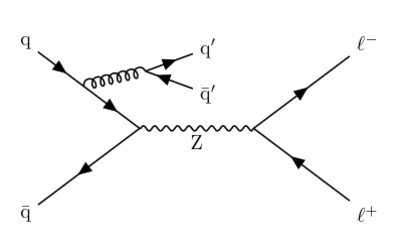
\includegraphics[width=0.4\textwidth]{figures/analysis/dy.pdf}
		\caption{The Feynman diagram for the dy background process.}
		\label{fig:dy_background}
	\end{figure}
	\item[] $\texttt{t}\bar{\texttt{t}}$: Production of top quark pairs $t\bar{t}$. These quarks decay with high probability via $t\rightarrow Wb$ and with the leptonic decay channel of the $W$, this has the same final state as the signal process and has a large background contribution. The corresponding Feynman diagram is shown in fig. \ref{fig:tt_background}.
	\begin{figure}[h!]
		\centering
		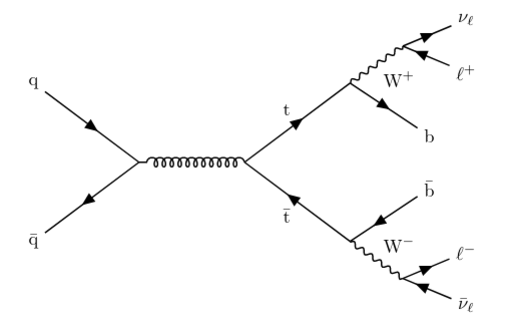
\includegraphics[width=0.5\textwidth]{figures/analysis/tt.pdf}
		\caption{The Feynman diagram for the tt background process.}
		\label{fig:tt_background}
	\end{figure}
 	\item[] $\texttt{st}$ and $\texttt{t}\bar{\texttt{t}}\texttt{V}$: Single top quark production and associated vector boson production with a $t\bar{t}$ pair. For the top quarks decaying into bottom quarks and leptonically decaying vector bosons, this yields a final state similar to the signal final state.
	\item[] \texttt{VV}, \texttt{VVV} and $\texttt{t}{\bar{\texttt{t}}}\texttt{VV}$: di- or triple boson production with (or without) associated $t\bar{t}$ production. If any of these vector bosons decay hadronically while the other(s) decay leptonically, this results in a leptonic final state.
	\item[] $\texttt{t}\bar{\texttt{t}}\texttt{VH}$, \texttt{ggH} and \texttt{VBFH} are Higgs production channels. \texttt{wjets} are leptonically decaying jet-associated $W$ boson production. \texttt{QCD} is QCD background. \texttt{rare} are rare processes (such as four top production) with individual low contribution each.
\end{itemize}

The list of the background samples from the MC simulations are all listed in tab. \ref{tab:bkg_datasets}.

\begingroup
\footnotesize
\setlength\LTleft{-1.0cm}
\begin{longtable}[b]{llS[table-format=9.0]S[table-format=7.8]}
	\caption{List of simulated background samples for 2017 with the cross section $\sigma$ of each process and the number of generated events $N$, divided into process groups. The symbol \texttt{*} is a placeholder for \texttt{pythia8}, while \texttt{**} denotes \texttt{inclusiveDecays}. Long dataset names are split into multiple lines, denoted by an indentation. (NanoAODv7, 102X\_mc2017\_realistic\_v8-v1)}\\
	Process&Dataset name&{N}&$\sigma/$\si{\pico\barn} \\
	\midrule
	\endfirsthead
	\toprule
	Process&Dataset name&{N}&$\sigma/$\si{\pico\barn} \\
	\midrule
	\endhead
	\bottomrule
	\endfoot
	\bottomrule
	\endlastfoot
	
	\multirow{ 4}{*}{DY}&\verb|DYJetsToLL_M-10to50_TuneCP5_13TeV-madgraphMLM-*| & 79058069&18610.0\\
	&\verb|DYJetsToLL_0J_TuneCP5_13TeV-amcatnloFXFX-*| &88134822 &4843.6\\
	&\verb|DYJetsToLL_1J_TuneCP5_13TeV-amcatnloFXFX-*| & 95629091&897.8\\
	&\verb|DYJetsToLL_2J_TuneCP5_13TeV-amcatnloFXFX-*| & 54497574&335.8\\
	\midrule%t$\bar{\textrm{t}}$
	\multirow{ 3}{*}{t$\Bar{\textrm{t}}$}&\verb|TTTo2L2Nu_TuneCP5_PSweights_13TeV-powheg-*| & 68296294&88.4\\
	&\verb|TTToSemiLeptonic_TuneCP5_PSweights_13TeV-powheg-*| & 109795512&365.52\\
	&\verb|TTToHadronic_TuneCP5_PSweights_13TeV-powheg-*| &128829950&377.96\\
	\midrule
	\multirow{ 5}{*}{VV}&\verb|WWTo2L2Nu_NNPDF31_TuneCP5_PSweights_13TeV-powheg-*| & 2000000&12.2\\
	&\verb|WWTo2L2Nu_DoubleScattering_13TeV-*| & 968000&0.2232\\
	&\verb|ZZTo4L_13TeV_powheg_*| & 207798469&1.256\\
	&\verb|WZTo3LNu_TuneCP5_13TeV-amcatnloFXFX-*| & 10987679&4.43\\
	&\verb|ZGToLLG_01J_5f_TuneCP5_13TeV-amcatnloFXFX-*| & 30490034&55.59\\
	\midrule
	%&\verb|?WGToLNuG_TuneCP5_13TeV-madgraphMLM-*| &  6283083&464.800\\%aktuell auskommentiert
	%\midrule
	\multirow{ 7}{*}{ST}&\verb|ST_t-channel_top_4f_**_TuneCP5_13TeV-powhegV2-madspin-*| & 5982064&136.02\\
	&\verb|ST_t-channel_antitop_4f_**_TuneCP5_13TeV-powhegV2-madspin-*| & 3675910&80.95\\
	&\verb|ST_s-channel_4f_leptonDecays_TuneCP5_| & 9914948&3.364\\
	&\verb|     PSweights_13TeV-amcatnlo-*|\\
	&\verb|ST_tW_top_5f_**_TuneCP5_PSweights_13TeV-powheg-*| &7755138 &35.85\\
	&\verb|ST_tW_antitop_5f_**_TuneCP5_PSweights_13TeV-powheg-*| & 7745276&35.85\\
	&\verb|ST_tWll_5f_LO_TuneCP5_PSweights_13TeV-madgraph-*| & 986000&0.01096\\
    \newpage
	%\midrule
	\multirow{ 5}{*}{VVV}&\verb|WWW_4F_TuneCP5_13TeV-amcatnlo-*| & 472300&0.2086\\
	&\verb|WWZ_4F_TuneCP5_13TeV-amcatnlo-*| & 500000&0.1676\\
	&\verb|WZZ_TuneCP5_13TeV-amcatnlo-*| & 500000&0.05701\\
	&\verb|ZZZ_TuneCP5_13TeV-amcatnlo-*| & 500000&0.01473\\
	&\verb|WZG_TuneCP5_13TeV-amcatnlo-*| & 1000000&0.04345\\
	\midrule
	\multirow{ 5}{*}{t$\Bar{\textrm{t}}$V}&\verb|TTZToLL_M-1to10_TuneCP5_13TeV-amcatnlo-*| &250000 &0.0822\\
	&\verb|TTZToLLNuNu_M-10_TuneCP5_PSweights_13TeV-amcatnlo-*| &11092000 &0.2814\\
	&\verb|TTZToQQ_TuneCP5_13TeV-amcatnlo-*| &9690000 &0.5868\\
	&\verb|TTWJetsToLNu_TuneCP5_PSweights_13TeV-amcatnloFXFX-madspin-*| & 9828579&0.196\\
	&\verb|TTWJetsToQQ_TuneCP5_13TeV-amcatnloFXFX-madspin-*| &811306 &0.4049\\
	\midrule
	\multirow{ 1}{*}{t$\Bar{\textrm{t}}$VV}&\verb|TTWW_TuneCP5_13TeV-madgraph-*| & 1162000&0.006981\\
	\midrule
	\multirow{ 2}{*}{t$\Bar{\textrm{t}}$VH}&\verb|TTWH_TuneCP5_13TeV-madgraph-*| & 200000&0.001582\\
	&\verb|TTZH_TuneCP5_13TeV-madgraph-*| & 200000&0.001535\\
	\midrule
	\multirow{ 9}{*}{ggH}&\verb|GluGluHToTauTau_M125_13TeV_powheg_*| &15072210 &3.0469\\
	&\verb|GluGluHToZZTo4L_M125_13TeV_powheg2_JHUGenV7011_*| &1953198&0.01297\\
	&\verb|GluGluHToZZTo2L2Q_M125_13TeV_powheg2_JHUGenV7011_*| &1992000 &0.17963\\
	&\verb|GluGluHToWWToLNuQQ_M125_NNPDF31_TuneCP5_| &465000 &4.5621\\
	&\verb|     PSweights_13TeV_powheg_JHUGen710_*|\\
	&\verb|GluGluHToWWTo2L2Nu_M125_13TeV_powheg2_JHUGenV714_*| &953600&1.1033\\
	&\verb|GluGluHToMuMu_M-125_TuneCP5_PSweights_13TeV_powheg_*| & 1983600&0.010571\\
	&\verb|GluGluHToBB_M125_13TeV_amcatnloFXFX_*| & 9358631&28.293\\
	&\verb|GluGluHToGG_M125_13TeV_amcatnloFXFX_*| & 3942252&0.11028\\
	\midrule
	\multirow{ 7}{*}{VBF}&\verb|VBFHToTauTau_M125_13TeV_powheg_*| & 2977152&0.2372\\
	&\verb|VBF_HToZZTo4L_M125_13TeV_powheg2_JHUGenV7011_*| & 2220820&0.0010099\\
	&\verb|VBFHToWWToLNuQQ_M125_NNPDF31_TuneCP5_| & 480000&0.35517\\
	&\verb|     PSweights_13TeV_powheg_JHUGen710_*|\\
	&\verb|VBFHToWWTo2L2Nu_M125_13TeV_powheg2_JHUGenV714_*| & 500000&0.085894\\
	&\verb|VBFHToMuMu_M-125_TuneCP5_PSweights_13TeV_powheg_*| & 982200&0.00082296\\
	&\verb|VBFHToBB_M-125_13TeV_powheg_*_weightfix| & 5000000&2.2026\\
	&\verb|VBFHToGG_M125_13TeV_amcatnlo_*_PSWeights| &975930 &0.0085851\\
	\midrule
	\multirow{ 8}{*}{WJets}&\verb|WJetsToLNu_HT-70To100_TuneCP5_13TeV-madgraphMLM-pythia8| & 22255124&1504.92\\
	&\verb|WJetsToLNu_HT-100To200_TuneCP5_13TeV-madgraphMLM-pythia8| &35862893&1625.08\\
	&\verb|WJetsToLNu_HT-200To400_TuneCP5_13TeV-madgraphMLM-pythia8| & 21250517&477.96\\
	&\verb|WJetsToLNu_HT-400To600_TuneCP5_13TeV-madgraphMLM-pythia8| &14313274&67.441\\
	&\verb|WJetsToLNu_HT-600To800_TuneCP5_13TeV-madgraphMLM-pythia8| & 21709087&15.096\\
	&\verb|WJetsToLNu_HT-800To1200_TuneCP5_13TeV-madgraphMLM-pythia8| & 20432728&6.3626\\
	&\verb|WJetsToLNu_HT-1200To2500_TuneCP5_13TeV-madgraphMLM-pythia8| & 20258624&1.2658\\
	&\verb|WJetsToLNu_HT-2500ToInf_TuneCP5_13TeV-madgraphMLM-pythia8| & 21495421&0.009405\\
	\midrule
	\multirow{ 5}{*}{rare}&\verb|WpWpJJ_EWK-QCD_TuneCP5_13TeV-madgraph-*| &149000 &0.04926\\
	&\verb|TTGJets_TuneCP5_13TeV-amcatnloFXFX-madspin-*| & 25290267&4.215\\
	&\verb|TGJets_leptonDecays_TuneCP5_PSweights_13TeV-amcatnlo-*| &6649547 &1.018\\
	&\verb|tZq_ll_4f_ckm_NLO_TuneCP5_PSweights_13TeV-amcatnlo-*| & 13276146&0.07358\\
	&\verb|TTTT_TuneCP5_PSweights_13TeV-amcatnlo-*| & 2273928&0.008213\\
	\midrule
	\multirow{ 8}{*}{QCD}
	&\verb|QCD_HT100to200_TuneCP5_13TeV-madgraph-*| &93231801&23590000.0\\
	&\verb|QCD_HT200to300_TuneCP5_13TeV-madgraph-*| & 59197363&1551000.0\\
	&\verb|QCD_HT300to500_TuneCP5_13TeV-madgraph-*| & 60258921&323400.0\\
	&\verb|QCD_HT500to700_TuneCP5_13TeV-madgraph-*| & 56207744&30140.0\\
	&\verb|QCD_HT700to1000_TuneCP5_13TeV-madgraph-*| & 47610552&6344.0\\
	&\verb|QCD_HT1000to1500_TuneCP5_13TeV-madgraph-*| & 33420390&1092.0\\
	&\verb|QCD_HT1500to2000_TuneCP5_13TeV-madgraph-*| & 11634434&99.76\\
	&\verb|QCD_HT2000toInf_TuneCP5_13TeV-madgraph-*| & 5941306&20.35\\
	\label{tab:bkg_datasets}	
\end{longtable}
\endgroup
\setlength\LTleft{0.0cm}

\Subsection{Analysis Setup}

In the following, the selected electron, muon and jet final state objects (reconstructed and identified by ParticleFlow) will be described in detail. First, the physics processes are simulated, followed by a detector simulation. The resulting objects undergo a final state selection, isolating phase space regions for maximizing signal sensitivity. Depending on the event signature, they are categorized and then organized into subcategories using a deep neural network, which assigns a probability score value to them. The resulting scores can be histogrammed and measured data can then be fitted to the resulting histogram. The analysis worfkflow has been summarized in fig. \ref{fig:analysis_workflow}.

\begin{figure}[h!]
	\centering
	\begin{tikzpicture}
		\tikzstyle{terminator} = [rectangle, draw, text centered, rounded corners, minimum height=3em]
		\tikzstyle{connector} = [draw, -latex']
		\node [terminator, fill=blue!20, text width=1.2cm] at (0,0) (start) {Monte Carlo};
		\node [terminator, fill=blue!20, text width=2cm] at (2.6,0) (detector) {Detector Simulation};
		\node [terminator, fill=blue!20, text width = 3cm] at (6.2,0) (cat) {Object selection\\Categorization};
		\node [terminator, fill=blue!20, text width = 2.5cm] at (10.2,0) (dnn) {DNN\\Subcategories};
		\node [terminator, fill=blue!20, text width = 1cm] at (13,0) (fit) {Fit};
		\path [connector] (start) -- (detector);
		\path [connector] (detector) -- (cat);
		\path [connector] (cat) -- (dnn);
		\path [connector] (dnn) -- (fit);
	\end{tikzpicture}
	\caption{Flow chart of the analysis workflow.}
	\label{fig:analysis_workflow}
\end{figure}

\Subsubsection{Final State Objects}

The muon selection criteria are listed in tab. \ref{tab:muon_selection}. For the muons, a $p_T$-cut of 15 GeV has been required. Furthermore, they ought to be identified as tight muons and have to be contained within the tracker. It is also required that their impact parameter (IP) geometry is compatible with the primary vertex (PV) too. In addition, the IP significance \texttt{sip3d} (defined as the ratio between the uncertainty of the IP and the IP itself) is also restricted to guarantee that these muons originate from the PV. The \texttt{pfRelISO04\_all} parameter cut ensures the isolation of the muons invoking a stronger constraint on their origin.

\begin{table}[h!]
	\centering
	\begin{tabular}{c}
		\hline
		\texttt{tightId} \\
		$p_T > \SI{15}{\giga\electronvolt}$ \\
		$|\eta| \leq 2.4$ \\
		$d_{xy} \leq \SI{0.05}{\centi\meter}$ \\
		$d_z \leq \SI{0.1}{\centi\meter}$ \\
		\texttt{sip3d} $\leq 8$ \\
		$\texttt{pfRelIso04\_all} \leq 0.15$  \\
		\hline \\
	\end{tabular}
	\caption{Selection criteria for muons.}
	\label{tab:muon_selection}
\end{table}

The electron selection criteria is listed in tab. \ref{tab:electron_selection}. The electrons are required to be contained in the tracker to ensure the quality of the transverse momentum reconstruction. These electrons should also originate from the primary vertex through the impact parameter (IP) cuts $d_i$. Similarly to muons, the IP significance and isolation measures are also restricted. For quality reconstruction, the maximum number of lost hits in the tracker is also limited. \texttt{MVA ID WP80} has been chosen and as identification efficiency the 80\% working point (WP80, defined on a Drell-Yan sample) has been selected.

\begin{table}[h!]
	\centering
	\begin{tabular}{c}
		\hline
		\texttt{MVA ID WP80} \\
		$p_T > \SI{15}{\giga\electronvolt} $\\
		$|\eta| \leq 2.5$ \\
		$d_{xy} \leq \SI{0.05}{\centi\meter}$ \\
		$d_z \leq \SI{0.1}{\centi\meter}$ \\
		$\texttt{pfRelIso04\_all} \leq 0.15$  \\
		sip3d $\leq 8$ \\
		$\text{lost hits} \leq 1$ \\
		\hline \\
	\end{tabular}
	\caption{Selection criteria for the electrons.}
	\label{tab:electron_selection}
\end{table}

For the jets in consideration, the selection criteria in tab. \ref{tab:jet_selection} are applied. The AK4 jets are required to carry the tight ID. In addition to that, they are restricted to the region covered by the tracker. Based on the jet selection, the flavour tracking algorithm identifies the bottom jets. For the AK4-tagging, DeepFlavour is used.

\begin{table}[h!]
	\centering
	\begin{tabular}{c}
		\hline
		\texttt{tightId} \\
		$p_T > \SI{30}{\giga\electronvolt}$ \\
		$|\eta| < 2.4$ \\
		\hline
	\end{tabular}
	\caption{Jet selection criteria applied to the AK4 jets.}
	\label{tab:jet_selection}
\end{table}

\Subsubsection{Event Selection and Categorisation}

The selected events have been categorized depending on their final state configuration. In the network analysis, only channels with two b tagged AK4 jets with one or two lepton final states have been chosen.

In the two lepton configurations, the lepton charges are required to be opposite, such that the total charge of selected objects is $Q_{tot} = 0$. In addition to that, the invariant mass defined by the dilepton system is required to be close to the $Z$ mass and only events with a maximum absolute deviation of $\SI{15}{\giga\electronvolt}$ are kept. For the one lepton channels, such selection is not possible. Additional selection with supplementary leading lepton transverse momentum $p^l_T$ and missing transverse energy $\slashed{E}_T$ cuts is performed. A summary of these selection criteria for the considered channels are listed in tab. \ref{tab:categories}.


\begin{table}[h!]
	\centering
	\begin{tabular}{ccccc}
		channel & $\mu\mu$ & $ee$ & $\mu$ & $e$ \\
		\hline \\
		$p^l_T$ & $>\SI{30}{\giga\electronvolt}$ & $>\SI{25}{\giga\electronvolt}$ & $>\SI{25}{\giga\electronvolt}$ & $>\SI{35}{\giga\electronvolt}$ \\
		$n_\mu$ & 2 & 0 & 1 & 0 \\
		$n_e$ & 0 & 2 & 0 & 1 \\
		$Q_{tot}$ & 0 & 0 & -- & -- \\
		$\slashed{E}_T$ & -- & -- & \multicolumn{2}{c}{$>\SI{30}{\giga\electronvolt}$}  \\
		$m_{ll}$ & \multicolumn{2}{c}{$|m_{ll}-m_Z|\leq\SI{15}{\giga\electronvolt}$} & -- & -- \\
	\end{tabular}
	\caption{Selected categories with the additional kinematic cuts they impose. Note that there is a channel for each trigger.}
	\label{tab:categories}
\end{table}

\Subsubsection{Multi-Process Classification and Weight Application}

Following the definition of the channels, the contained events are further categorized using a deep neural network (DNN). The network assigns these events to so-called subcategories within each channel. The input variables include properties of additional physics objects, such as AK8 jets, the physics object kinematic variables, correlations among them and additional jet and particle identification values. %The complete list of input variables is shown in tab. \ref{tab:DNN_inputs}.

\begin{comment}
\begin{table}[h!]
	\centering
	\begin{tabular}{cc}
		Object & Variable \\
		\hline
		Leptons (2) & $E, p_x, p_y, p_z, q$, PDG ID \\
		AK4 jets (4) & $E, p_x, p_y, p_z$, b-tag value \\
		AK8 jets (2) & $E, p_x, p_y, p_z$, b-tag value \\
		Correlated objects & $m_{ll}, \Delta\phi_{jj}, \Delta R_{ll}$ \\
		                   & $m_{jj}, p_{T, jj}, \Delta\phi_{jj}, \Delta R_{jj}$ \\
		                   & $\min(\Delta R_{l1j1}, \Delta R_{l1j2})$ \\
		                   & $\min(\Delta R_{l2j1}, \Delta R_{l2j2}$ \\
		                   & $m_{lljj}, N_{AK4j}, p^{miss}_T$
	\end{tabular}
	\caption{The 54 inputs of the classifier DNN with object multiplicity indicated in brackets. Note that the network has been trained as a general final state classifier, so additional kinematic variables irrelevant for the dilepton and single lepton channel analysis are also used as inputs.}
	\label{tab:DNN_inputs}
\end{table}
\end{comment}

The DNN assigns a probability to each event belonging to a process group. As the sensitivity for some rarely occuring background processes is low, these are grouped together into a common process group. Hence, for the 16 processes the analysis differentiates between there are only 13 process groups, which the DNN sorts the events into. The 13 process groups are listed in tab. \ref{tab:DNN_outputs}.

The events carry a generator weight, as it would be computationally infeasible to simulate all processes proportionally to their occurrence and have to be scaled with the experiment luminosity and process cross section. The resulting weights written as

\begin{equation*}
	w_i = \frac{\mathcal{L}\sigma w^\text{gen}_i}{\sum\limits_i w^\text{gen}_i}
\end{equation*}

with luminosity $\mathcal{L}$ and cross section $\sigma$ and are then applied to the maximum DNN score distribution histogram following the classification for each event $i$.

\begin{table}[h!]
	\centering
	\begin{tabular}{cc}
		Process group & Included Processes \\
		\hline
		\texttt{ggZH} & \texttt{ggZH} \\
		\texttt{ZH\_DY} & \texttt{ZH\_DY} \\
		\texttt{WH} & \texttt{WH} \\
		\texttt{dy} & \texttt{dy} \\
		\texttt{tt} & \texttt{t}$\bar{\texttt{t}}$ \\
		\texttt{st} & \texttt{st} \\
		\texttt{ggH} & \texttt{ggH} \\
		\texttt{VBFH} & \texttt{VBFH} \\
		\texttt{wjets} & \texttt{wjets} \\
		\texttt{QCD} & \texttt{QCD} \\
		\texttt{merged\_ttVX} & \texttt{t}$\bar{\texttt{t}}$\texttt{V}, \texttt{t}$\bar{\texttt{t}}$\texttt{VV},  \texttt{t}$\bar{\texttt{t}}$\texttt{VH} \\
		\texttt{merged\_multiboson} & \texttt{VV}, \texttt{VVV} \\
	\end{tabular}
	\caption{The output nodes of the DNN corresponding to a single process group each. Note that some process groups contain multiple rare processes which are difficult to resolve.}
	\label{tab:DNN_outputs}
\end{table}

An example output of a such classification is shown for an $ee$ category and \texttt{ZH\_DY} output node in fig. \ref{fig:ZH_DY_sub}. In total, there are $13\times4 = 52$ cases for the 13 output nodes and 4 categories. On this particular plot, the strong Drell-Yan and $t\bar{t}$ background is clearly visible, with \texttt{ZH\_DY} having the highest share among the signal processes.

\begin{figure}[h!]
	\centering
	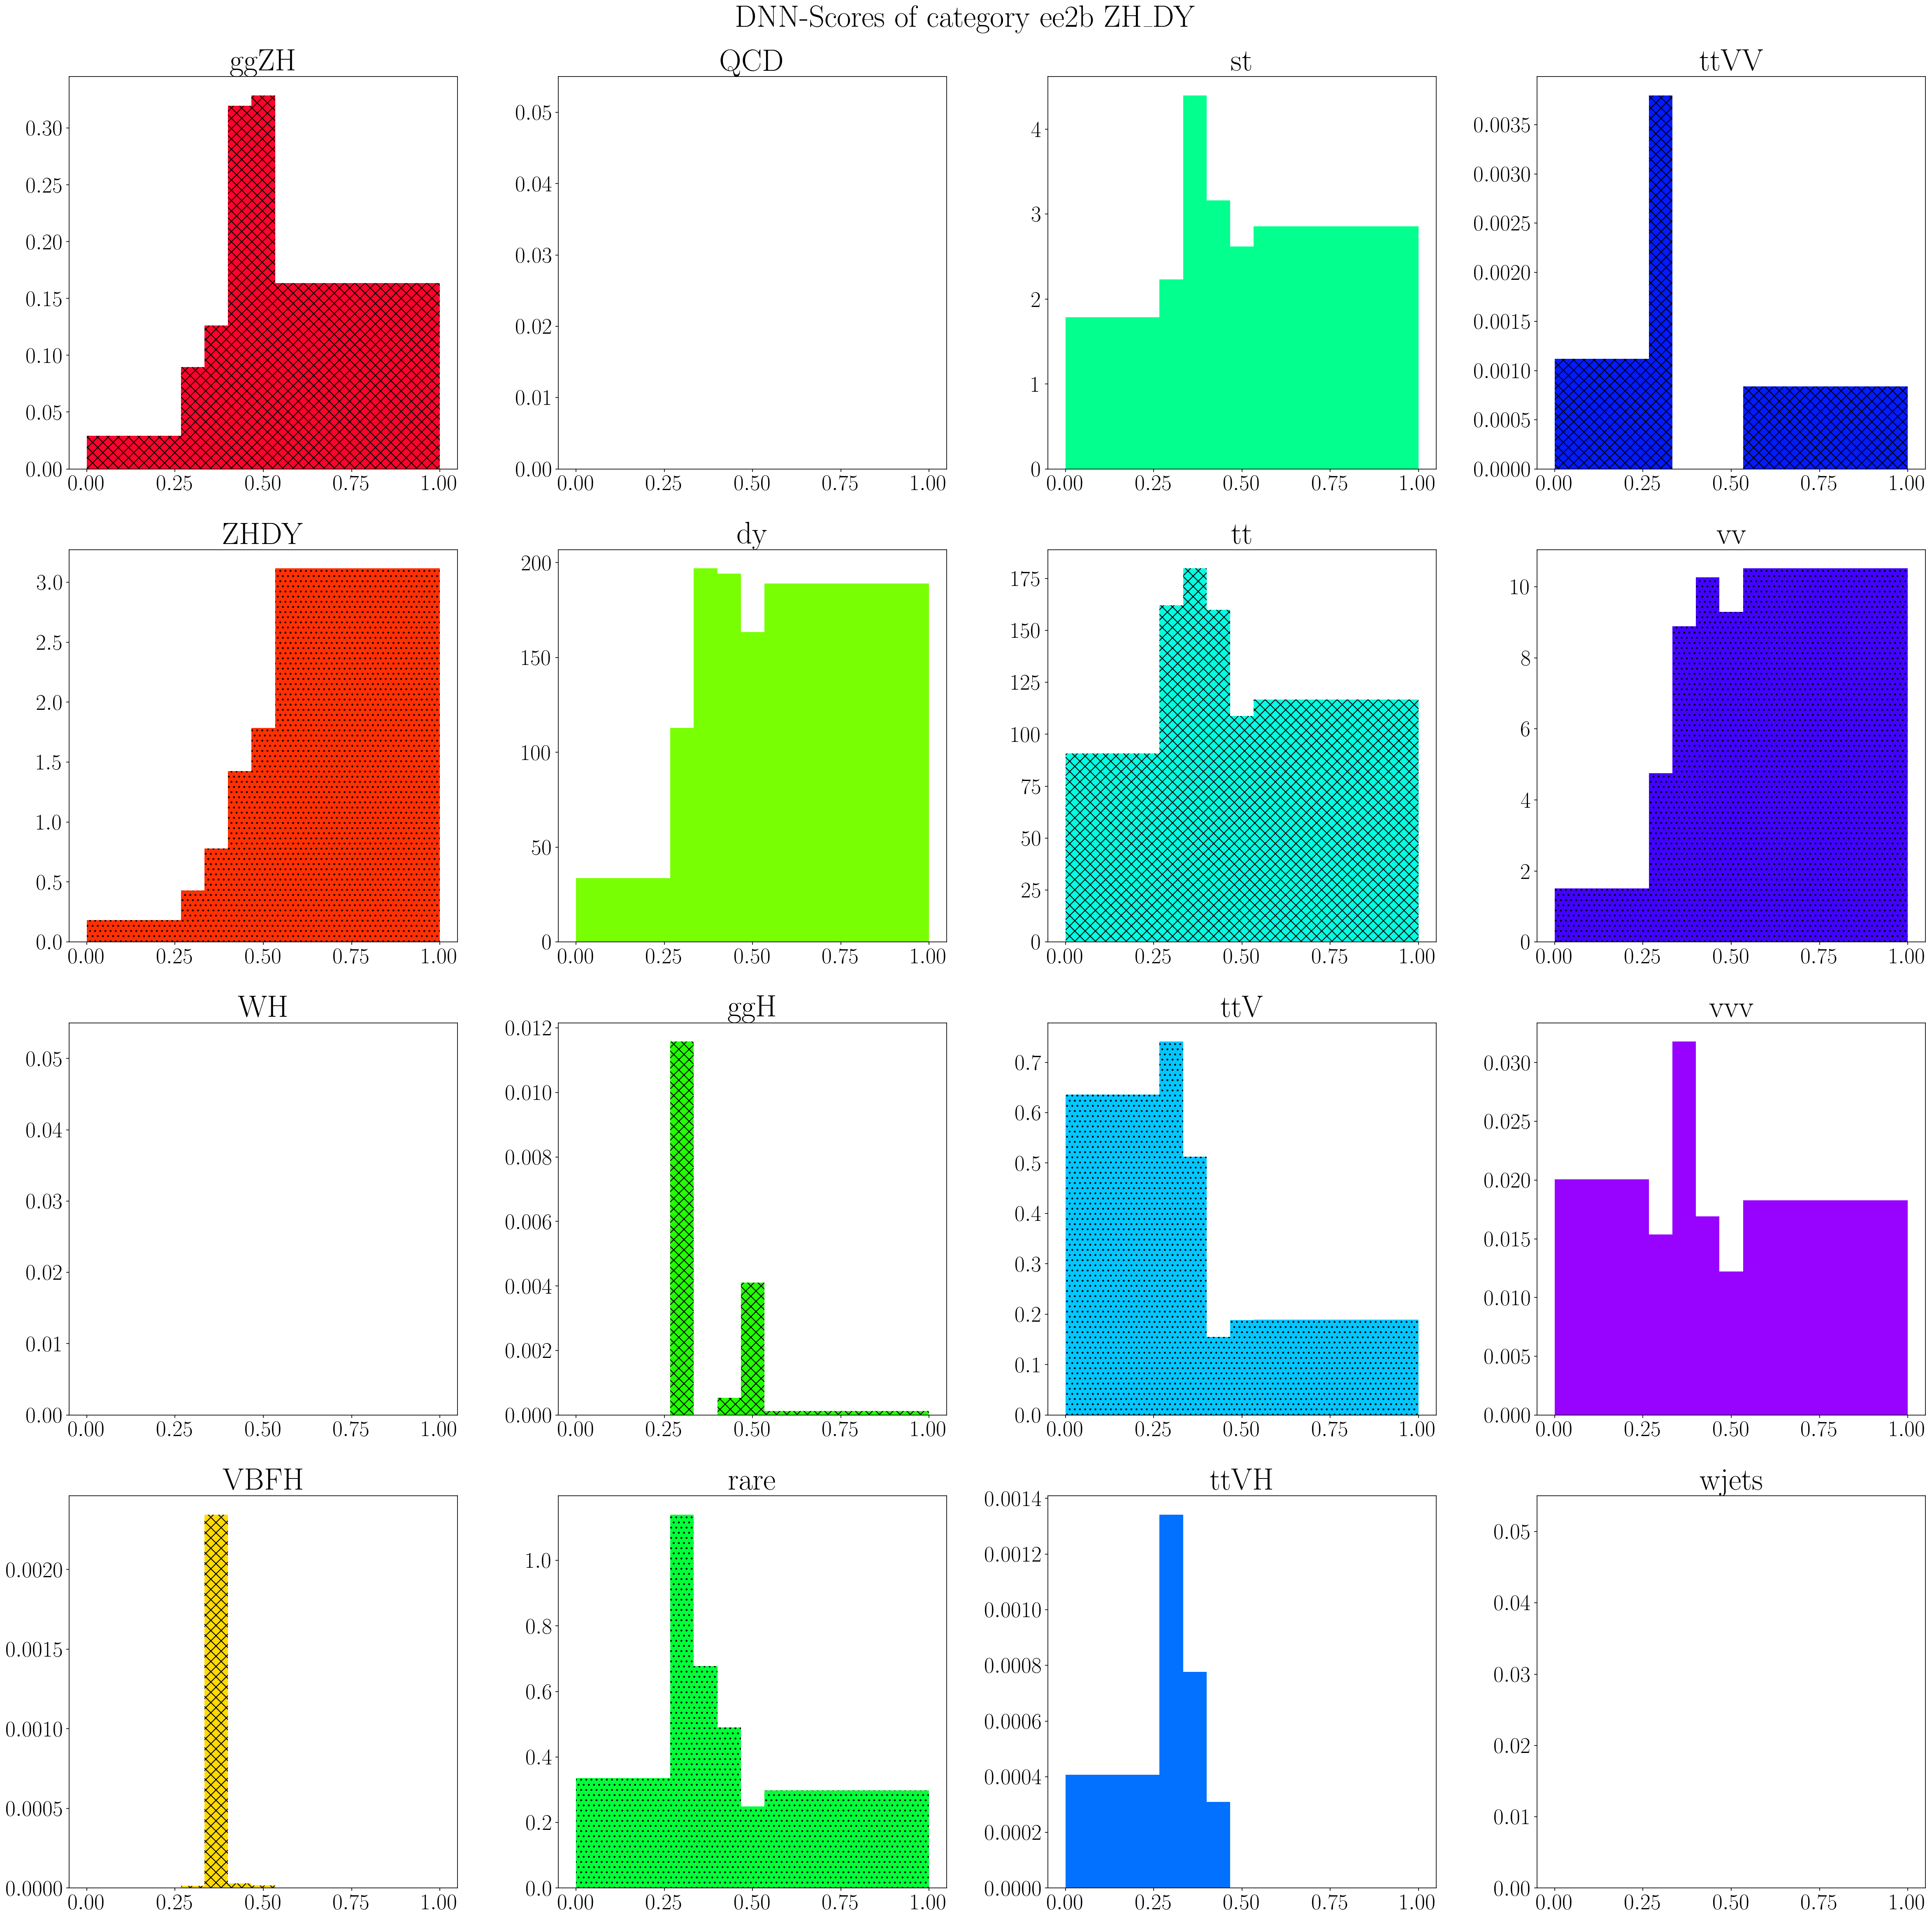
\includegraphics[width=\linewidth]{figures/analysis/ee_2b_dnn_node_ZH_DY.png}
	\caption{The DNN score distribution for the categorised final state objects for the \texttt{ZH\_DY} subcategory. Note the the different norming of the y axis and the high share of $t\bar{t}$, \texttt{dy} and \texttt{ZH\_DY} processes. Due to the effective categorization none of the \texttt{WH}, \texttt{QCD} and \texttt{wjets} events landed in this category. This is one of the total 52 subcategories.}
	\label{fig:ZH_DY_sub}
\end{figure}

The DNN probability score distribution of every category can be fitted to data. A such distribution for a single category is shown in fig. \ref{fig:ee_dnn_score}; for all four categories covered by this study, the resulting histogram in shown in fig. \ref{fig:conditions}. In case of a measured dataset, only the resulting bin count would be visible on which an analytical likelihood fit can be performed.

\begin{figure}[h!]
	\centering
	\includegraphics[width=\linewidth]{figures/analysis/cond1.png}
	\caption{The DNN score histogram distribution for the $ee$ category and each 13 subcategory (separated in red). On the x-axis, only the bin index is shown. The fourth subcategory from the left corresponds to the above-mentioned \texttt{ZH\_DY} subcategory. The \texttt{ggZH} subcategory is the seventh from the left with the two bins. This is one of the four channels.}
	\label{fig:ee_dnn_score}
\end{figure}

\begin{figure}[h]
	\centering
	\includegraphics[width=1.1\linewidth]{figures/analysis/cond4_notOrdered.png}
	\caption{The distribution of the DNN scores for each subcategory (separated in red) in the one and two lepton categories in consideration (separated in blue). Note the high share of Drell-Yan, $t\bar{t}$ and QCD background events in each bin and the absence of $WH$ events in the two lepton bins. The $ee$ category is the second one from the left.}
	\label{fig:conditions}
\end{figure}

\Subsubsection{Likelihood Fits}

Using these histograms, a maximum likelihood fit can be performed to determine the signal strength parameters. For that, the likelihood function for a signal+background hypothesis is defined, which can be written as

\begin{equation*}
	\mathcal{L}(N | \left\{\mu_i\right\} , \left\{\theta_i\right\}) = \prod\limits_i \frac{(\mu_is_i(\theta)+b_i(\theta))^N}{N!}e^{-\mu_is_i(\theta) + b_i(\theta)} \prod\limits_j p(\tilde{\theta}_j | \theta_j)
\end{equation*}

The binwise signal and background contributions $s_i$ and $b_i$ depend on the uncertainty-modelling nuisance parameter $\theta$ and are Poisson-distributed; the nuisance parameters follow the probability distribution $p(\tilde{\theta} | \theta)$. This likelihood function is fitted to the histogram and encodes the variations of the background processes within the uncertainties.

In this thesis, these signal strength modifier parameters will inferred using a conditional invertible neural network and will be compared to their maximum likelihood counterpart.

% network architecture
\pageshift
\thispagestyle{plain}
\Section{Network Setup}

In this chapter the cINN setup will be discussed. In the first half, the generation of training and test datasets is going to elaborated, with a detailed focus on the analysis specifics, such as interpolation between histograms (morphing) and the representation of the statistic and systematic uncertainties.

In the second half of this chapter, the final cINN architecture used for the inference is going to be presented. The results of the inference and the interpretation of the network outputs will be discussed in the next chapter.

\Subsection{Training Dataset Generation}

The conditions shown in fig \ref{fig:conditions} in chapter \ref{ch:analysis_strategy} represent the expectation on the measured dataset. Unfortunately, the share of each process in each bin in the measured data is a priori unknown (which would mean the complete physics is known to the very last detail). For this purpose the different scenarios of a process having more or less shares in a bin have to be first artificially represented in the dataset in order to obtain a cINN which is capable of inferring the share of each process -- or in other words, to obtain the signal modifier parameters $\mu_i$.

\Subsubsection{Prior Selection}

In order to do so, a set of signal modifier parameters are drawn from a pool of expected parameter distribution (the prior). Then, each process in the histogram is scaled with the corresponding parameter and the bins will summed up meaning (similar to the expected dataset) the information about the contribution of each process to each bin is lost.

The prior distribution for the processes have been selected as the following. For the signal processes \texttt{ggZH}, \texttt{ZHDY} and \texttt{WH} the $\mu_i$ were sampled from a gamma distribution

\begin{equation*}
	f(x; k, \theta) = \frac{x^{k-1}e^{-x/\theta}}{\theta^k\Gamma(k)}
\end{equation*}

with shape parameter $k$ and scale $\theta$. An advantage of this distribution as prior is the positiveness of the samples $\{x_i\}$ from the distribution; apart from that, the distribution has a long tail for increasing values of $x$ which allow a more fined selection in a given range. The parameters were set to be $k = 1.5$ and $\theta = 7$; with this specific selection, one obtains a prior which is sensitive in the low signal yield region $\mu \lesssim 10$ while maintaining network sensitivity for values $\mu<100$.

For the background processes, it is expected that the MC simulations follow the expectation with good accuracy. Hence, one expects $\mu \approx 1$. For this reason, the prior has been chosen to follow a lognormal distribution

\begin{equation*}
	f(x; \mu, \sigma) = \frac{1}{\sqrt{2\pi }\sigma x}\exp\left(-\frac{\left(\ln(x)-\mu\right)^2}{2\sigma^2}\right)
\end{equation*}

with mean $\mu = 0.05$ and $\sigma = 0.25$, lognormal distributions being positive themselves.

In order the estimate the arising uncertainty from the luminosity, the obtained conditions (after scaling and uncertainty variation) are then scaled with an additional luminosity factor. These have been drawn from a lognormal distribution with $\mu = 0$ and $\sigma = 0.02$.
All distributions are shown in fig. \ref{fig:priors}.

\begin{figure}[h!]
	\centering
	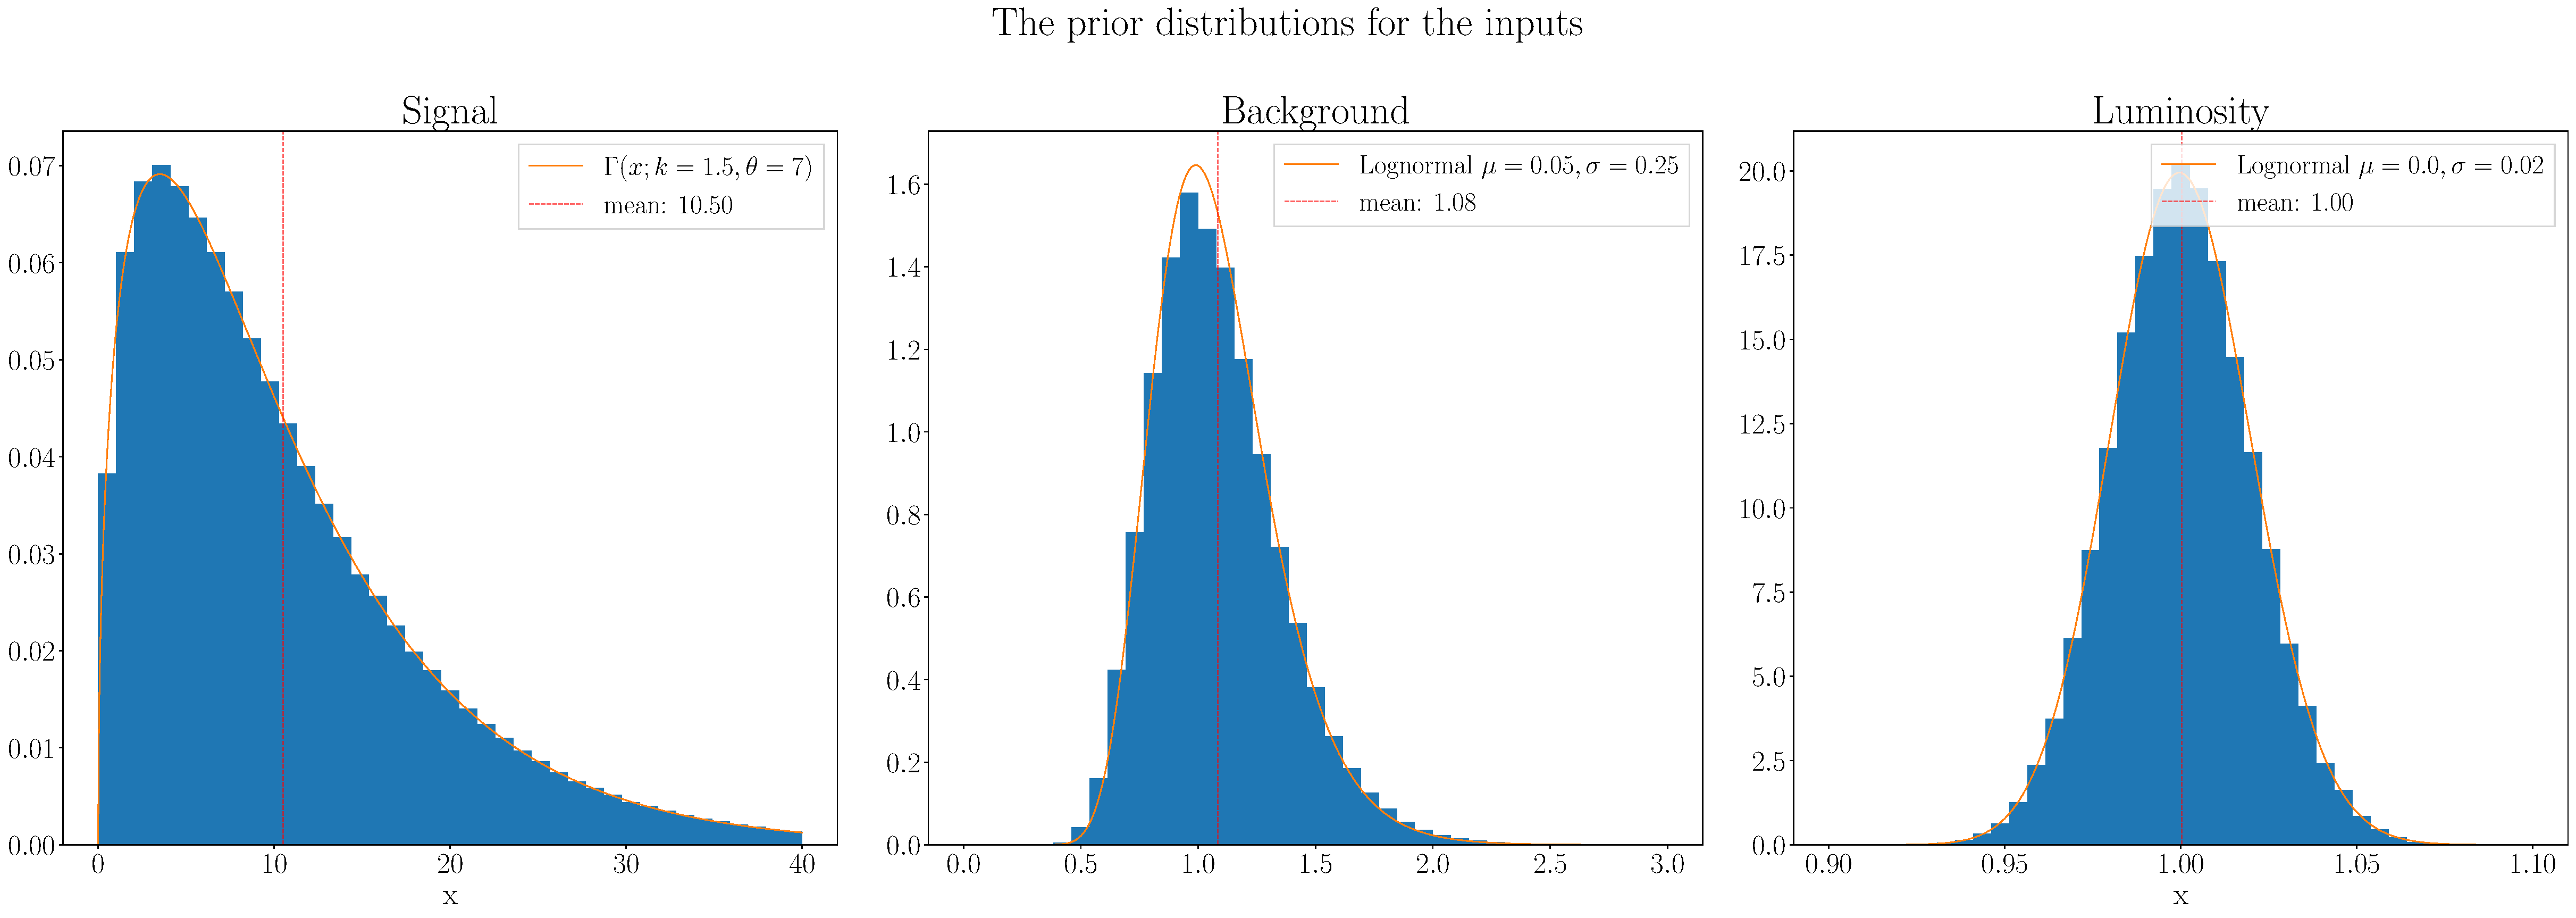
\includegraphics[width=\linewidth]{figures/network_setup/priors.pdf}
%	\begin{minipage}{.5\textwidth}
%		\centering
%%		\includegraphics[width=0.8\linewidth]{figures/network/signal}
%	\end{minipage}%
%	\begin{minipage}{.5\textwidth}
%		\centering
%%		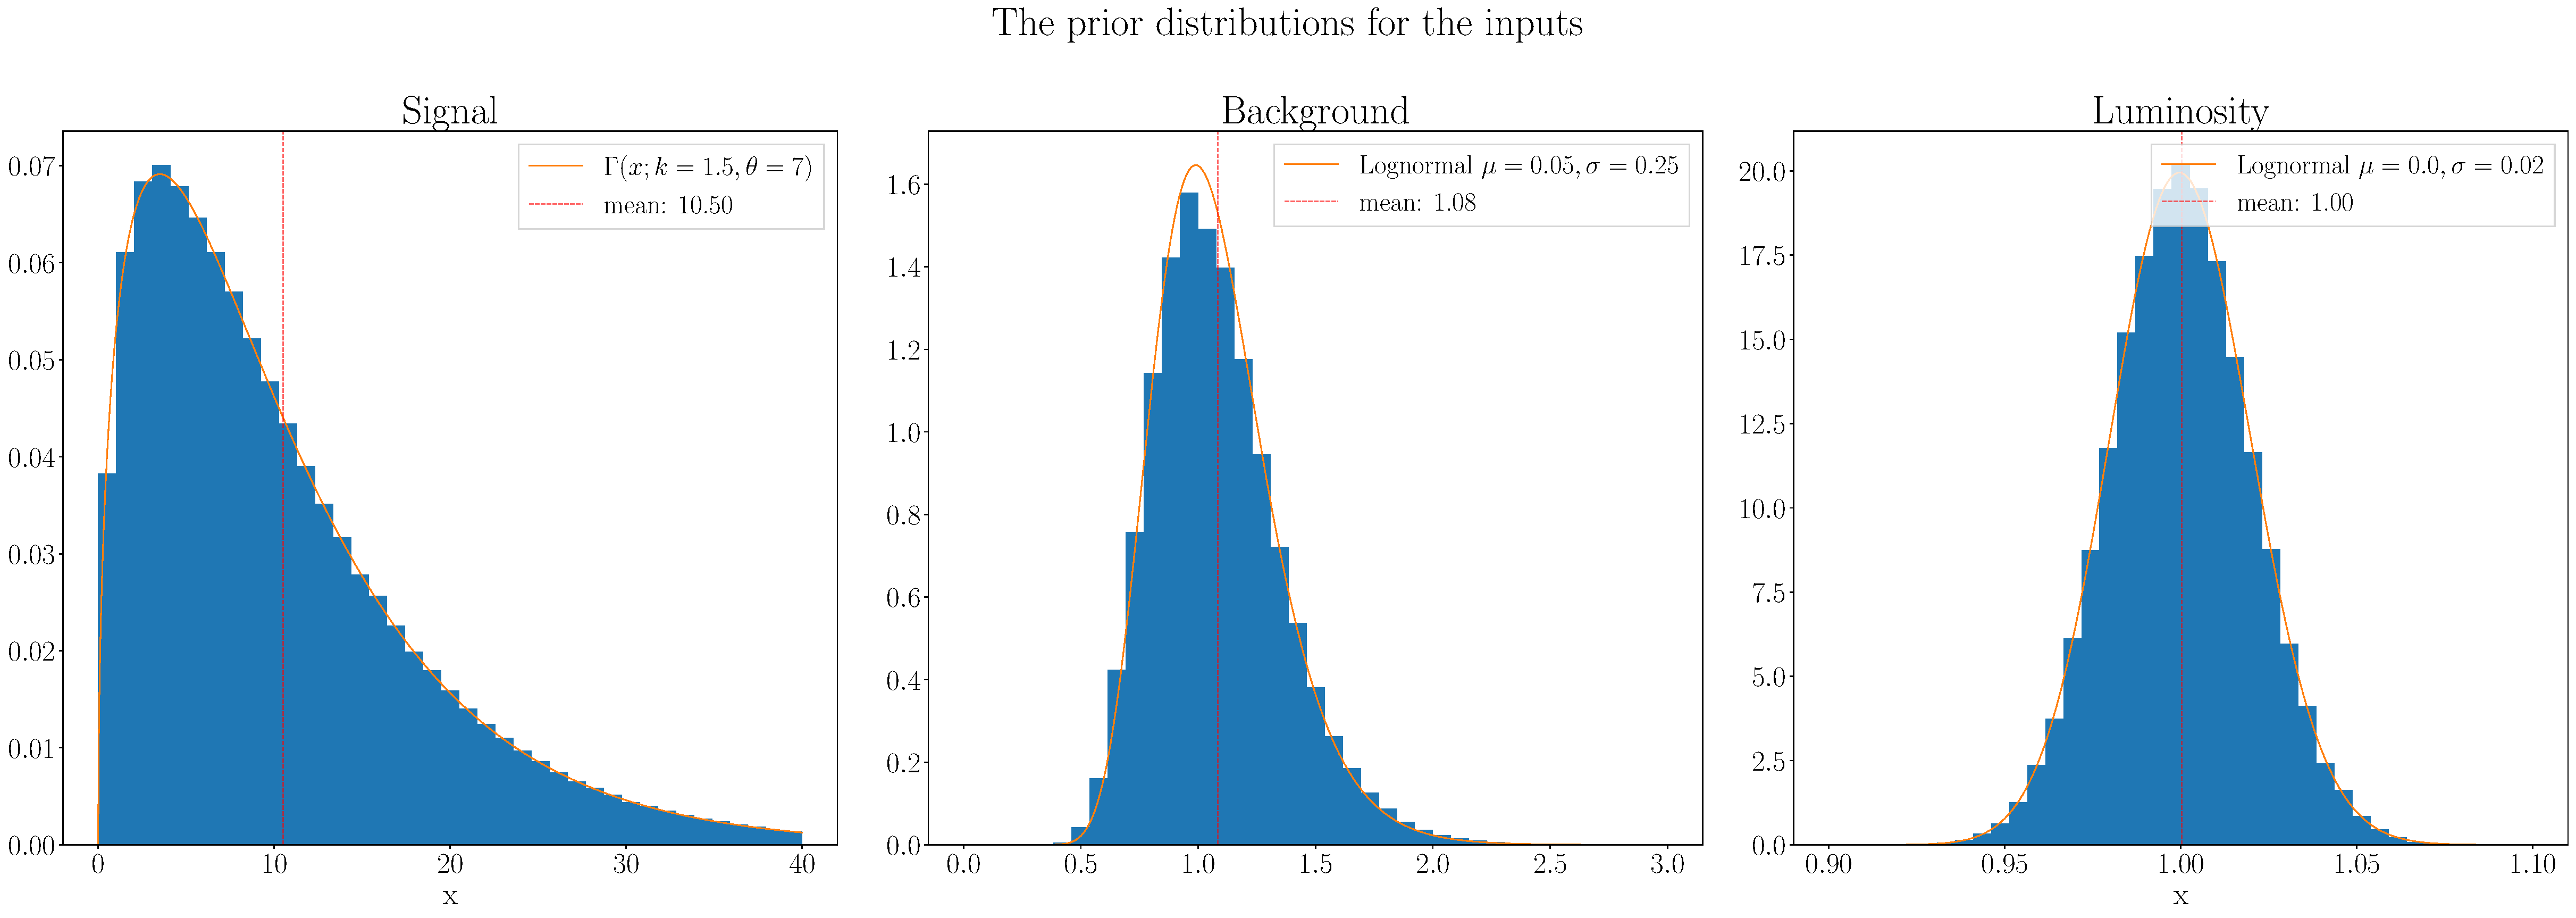
\includegraphics[width=0.6\linewidth]{figures/network_setup/priors.pdf}
%	\end{minipage}
	\caption{Prior distributions for the signal and background processes. Samples are shown in blue; the mean of each distribution is shown with the red dashed line. The analytic shape of each distribution is shown in orange.}
	\label{fig:priors}
\end{figure}

After successful histogram scaling, the statistical and systematic uncertainty fluctuations are applied to the scaled histogram.

\Subsection{Systematic Uncertainties}

\textcolor{red}{There are 24 sources of systematic uncertainties which have been taken into account. These are:} \\

%\begin{tabular}{c}
%	\texttt{PDFSet               }  \\
%	\texttt{PSWeight\_FSR        }  \\
%	\texttt{PSWeight\_ISR        }  \\
%	\texttt{ScaleWeight\_Envelope}  \\
%	\texttt{ScaleWeight\_Fact    }  \\
%	\texttt{ScaleWeight\_Mixed   }  \\
%	\texttt{ScaleWeight\_Renorm  }  \\
%	\texttt{btagWeight\_cferr1   }  \\
%	\texttt{btagWeight\_cferr2   }  \\
%	\texttt{btagWeight\_hf       }  \\
%	\texttt{btagWeight\_hfstats1 }  \\
%	\texttt{btagWeight\_hfstats2 }  \\
%	\texttt{btagWeight\_lf       }  \\
%	\texttt{btagWeight\_lfstats1 }  \\
%	\texttt{btagWeight\_lfstats2 }  \\
%	\texttt{electron\_id         }  \\
%	\texttt{electron\_reco       }  \\
%	\texttt{l1\_ecal\_prefiring  }  \\
%	\texttt{muon\_id             }  \\
%	\texttt{muon\_iso            }  \\
%	\texttt{pileup               }  \\
%%  \texttt{trigger\_e\_sf       }  \\
%	\texttt{trigger\_ee\_sf      }  \\
%	\texttt{trigger\_mu\_sf      }  \\
%	\texttt{trigger\_mumu\_sf    }  \\
%%  \texttt{top\_pT\_reweighting }  \\
%%  \texttt{TuneCP5              }  \\
%\end{tabular} 

The systematic uncertainties require an interpolation method as the shifts in the histograms are computationally expensive to obtain. In other words, as only the effect of the $1\sigma$ up- and down-shifts of the uncertainties (templates) listed above are given, the task to represent the in-between-cases (and obviously, those of outside of the given range) in the histrograms remains. For this purpose, a non-linear histogram morphing method has been implemented.

In the following, an overview of the morphing algorithm will be given with a discussion on the implementation and on its effects on the histograms following thereafter.

\Subsubsection{Non-linear Histogram Morphing}

Non-linear histogram morphing has been implemented on the basis of \cite{Baak_2015}. For the interpolation a nominal distribution and -- in this case -- 24 other distribution templates representing the $1\sigma$ and $-1\sigma$ shifts are given. The nominal template $f(x|m)$ with morphing parameter $m$ can then be appromated around $m=0$ with the other templates in a simple 1D case using

\begin{equation*}
	f(x|m) \approx \sum_j \left.\frac{\partial^{(j)} f(x|m)}{\partial m^{(j)}}\right|_{m=0}\frac{m^j}{j!} = \sum_j f_j'(x|m=0) m^j
\end{equation*}



where the derivatives and the factorials have been absorbed in $f'_j$.

For $T$ uncorrelated uncertainties (hence for $T$ morphing parameters $m$) with morphing parameter values $\pm1$ there are $2T+1$ sampled distributions in total (counting the nominal distribution). An intuitive representation of the "morphing parameter space" with the indication of the available templates is shown in fig. \ref{fig:morphing_phase_space}.

\begin{figure}[h!]
	\centering
	\centering
	\begin{tikzpicture}[scale=2]
		\coordinate (O) at (0,0,0);
		\draw[thick,->] (-1.,0,0) -- (1.,0,0) node[right=2]{$x$};
		\draw[thick,->] (0,-1,0) -- (0,1,0) node[right=-1]{$z$};
		\draw[thick,->] (0,0,-1.4) -- (0,0,1.4) node[below left=0.5]{$y$};
		
		\node[circle, fill=gray] (0) {};
		\node[circle, fill=gray] at (   0,-0.7, 0) {};
		\node at (0.8, -0.7, 0) {$m=(0,0,-1)$};
		\node[circle, fill=gray] at (   0, 0.7, 0) {};
		\node at (-1.2, 0.2, -1.4) {$m=(0,0,1)$};
		\node[circle, fill=gray] at (   0, 0  ,-1) {};
		\node at (-0.8, 0.2, 0) {$m=(-1,0,0)$};
		\node[circle, fill=gray] at (   0, 0  , 1) {};
		\node at (1, -0.2, 0) {$m=(1,0,0)$};
		\node[circle, fill=gray] at (-0.6, 0  , 0) {};
		\node at (-1.1, -0.4, 0) {$m=(0,1,0)$};
		\node[circle, fill=gray] at ( 0.6, 0  , 0) {};
		\node at (1.1, 0.4, 0) {$m=(0,-1,0)$};
	\end{tikzpicture}
	\caption{The morphing "phase space" showing the available distributions for $T=3$ uncertainties of $\sigma=\pm1$. The available templates in the phase space are shown in grey. Note that the nominal template with $m=(0,0,0)$ lies in the origin and there are no "mixed" templates (such as $m = (1,1,0)$) available. In the setting described above, one has $T=24$, hence there are $24\times2 +1 = 49$ templates in total.}
	\label{fig:morphing_phase_space}
\end{figure}

For theis multidemensional case as there are no "mixed templates" taking into account the effect of two independent systematic variations, the mixed derivative terms from the above expansion are zero. Hence, the expression can be written for a given $\mathbf{m}_i$\footnote{$\mathbf{m}_i = (0, 0, ..., 0, \pm 1, 0, ..., 0)$ for the i-th template with $\sigma=\pm1$} as:

\begin{equation}
	f(x | \mathbf{m}_i) = \underbrace{\vphantom{\frac{1}{2!}\left.\frac{\partial^2 f(x | \mathbf{m})}{\partial m_j^2}\right|_{\mathbf{m}=0}}f(x | 0)}_{f_0} + \sum^T_{j=1} \underbrace{\vphantom{\frac{1}{2!}\left.\frac{\partial^2 f(x | \mathbf{m})}{\partial m_j^2}\right|_{\mathbf{m}=0}}\left.\frac{\partial f(x | \mathbf{m})}{\partial m_j}\right|_{\mathbf{m}=0}}_{f'_j}(m_i)_j + \sum^T_{j=1} \underbrace{\frac{1}{2!}\left.\frac{\partial^2 f(x | \mathbf{m})}{\partial m_j^2}\right|_{\mathbf{m}=0}}_{f'_{jj}}(m_i)^2_j + \mathcal{O}\left((m_i)_j^3\right)
	\label{eq:morphing}
\end{equation}

where $(m_i)_j$ denotes the j-th component of the i-th morphing parameter vector. The aim is to find an expression for the unknown derivatives as only the histogram $f(x|m)$ is given. If one knew the derivatives, one could easily select a general $m_i$ and insert in into eq. \ref{eq:morphing}, yielding the morphed distribution.

In order to express the derivatives write all given templates in a vectorized form, and make use of the matrix form

\begin{equation*}
	\left(\begin{aligned}
		f\Bigl(x &| (0,\phantom{-}0, 0\,,...,\phantom{-}0)\Bigl) \\
		f\Bigl(x &| (0,\phantom{-}1, 0\,,...,\phantom{-}0)\Bigl) \\
		f\Bigl(x &| (0,-1, 0\,,...,\phantom{-}0)\Bigl) \\
		&\vdots \\
		f\Bigl(x &| (0,\phantom{-}0, 0\,,...,\phantom{-}1\Bigl) \\
		f\Bigl(x &| (0,\phantom{-}0, 0\,,...,-1\Bigl) \\
	\end{aligned}\right) = \underbrace{\left(\begin{matrix}
		1 & 0 & 0 & 0 & & 0 & 0 \\
		1 & 1 & 1 & 0 &  \cdots & 0 & 0 \\
		1 & -1 & 1 & 0 &      & 0 & 0 \\
		& & \vdots & & \ddots & \vdots & \\
		1 & 0 & 0 & 0 &       & 1 & 1 \\
		1 & 0 & 0 & 0 & \cdots & -1 & 1 \\
	\end{matrix}\right)}_{M} \left(\begin{matrix}
	f_0 \\
	f'_1 \\
	f'_{11} \\
	\vdots \\
	f'_T \\
	f'_{TT}
\end{matrix}\right)
\end{equation*}

With an invertible coefficient matrix $M \in \mathbb{R}^{49\times49}$, encoding the position of the templates in the morphing phase space. Inverting $M$\footnote{Note that thanks to the block matrix structure the inversion is computationally feasible. In addition, the inverse has to be evaluated only once.}

\begin{equation*}
	M^{-1} = \left(\begin{matrix}
		 1 & 0   & 0   & 0 &        & 0 & 0 \\
		 0 & 0.5 &-0.5 & 0 & \cdots & 0 & 0 \\
		-1 & 0.5 &\phantom{-}0.5 & 0 &        & 0 & 0 \\
		   & \vdots &     &    & \ddots &  & \vdots \\
		 0 & 0   & 0   & 0 &        & 0.5 & -0.5 \\
		-1 & 0   & 0   & 0 & \cdots & 0.5 & \phantom{-}0.5 \\
	\end{matrix}\right)
\end{equation*}

this collapses into

\begin{equation*}
	M^{-1}\mathbf{f} = \mathbf{f}'
\end{equation*}

and eq. \ref{eq:morphing} can be then written for a general $m$ as

\begin{equation}
	f(x|\mathbf{m}) = (1, m_1, m_1^2, ..., m_T, m^2_T) M^{-1}\mathbf{f}
	\label{eq:final_morphing}
\end{equation}

Eq. \ref{eq:final_morphing} is the final shape of the morphing algorithm implemented for the representation of the systematic effects in the dataset. The effect of the morphing algorithm on some samples is discussed in the next chapter.

\Subsubsection{\textcolor{red}{Systematic Uncertainty Representation}}

\Subsection{Statistical Uncertainties}

There are two sources of statistical uncertainties on Monte Carlo level. First, there is a Poisson fluctuation due to the generator generating a finite amount of samples for each process. As the number of samples is large, one can assume that these fluctuations follow a normal distribution. Second, it is expected that the data in the DNN-score histograms follow a Poisson distribution themselves.


\Subsection{Network Architecture}

In the following, the cINN network architectures for the inference will be elaborated.

The network inputs are one signal modifier parameter per process and an additional parameter representing the scaling due to the luminosity uncertainties. In total, the network has 17 inputs.

Regarding the conditions, it had a dimension of 235 for the four considered categories ($e$, $ee$, $\mu$ and $\mu\mu$).

The cINN uses 12 GLOW blocks. After each block, an additional permutation layer is introduced. These layers perform arbitrary (but fixed) permutations among the outputs. Note that this transformation has per construction a determinant of $\pm1$ making no change in the volume for the resulting normalizing flow. On the other hand, it does remove any correlations between neighbouring input values, making training more performant.

The GLOW networks contain subnetworks with 128 Nodes, of 4 layers. The activation function for each layer was chosen to be ReLU.

For the summary network studies, a shallow network has been constructed, as more complex setups tended to overtrain in the considered cases. The network had a layer of 300 nodes between the DNN scores and the condition node; the output dimensionality has been chosen to be 100.

Both networks have been trained for \textcolor{red}{11000 epochs} on a dataset containing 1.5 million generated samples. For training, a batchsize of 500 has been chosen. For the test set, 150 000 samples have been generated.

As a learning rate scheduler, an empirically well-functioning cosine scheduler has been used. This scheduler starts off with a learning rate of $10^{-3}$ and reduces it to $10^{-5}$ in steps in each epoch. The evolution of the learning rate is shown in fig. \ref{fig:lr}. As an optimizer, Adam has been chosen.

\begin{figure}
	\centering
	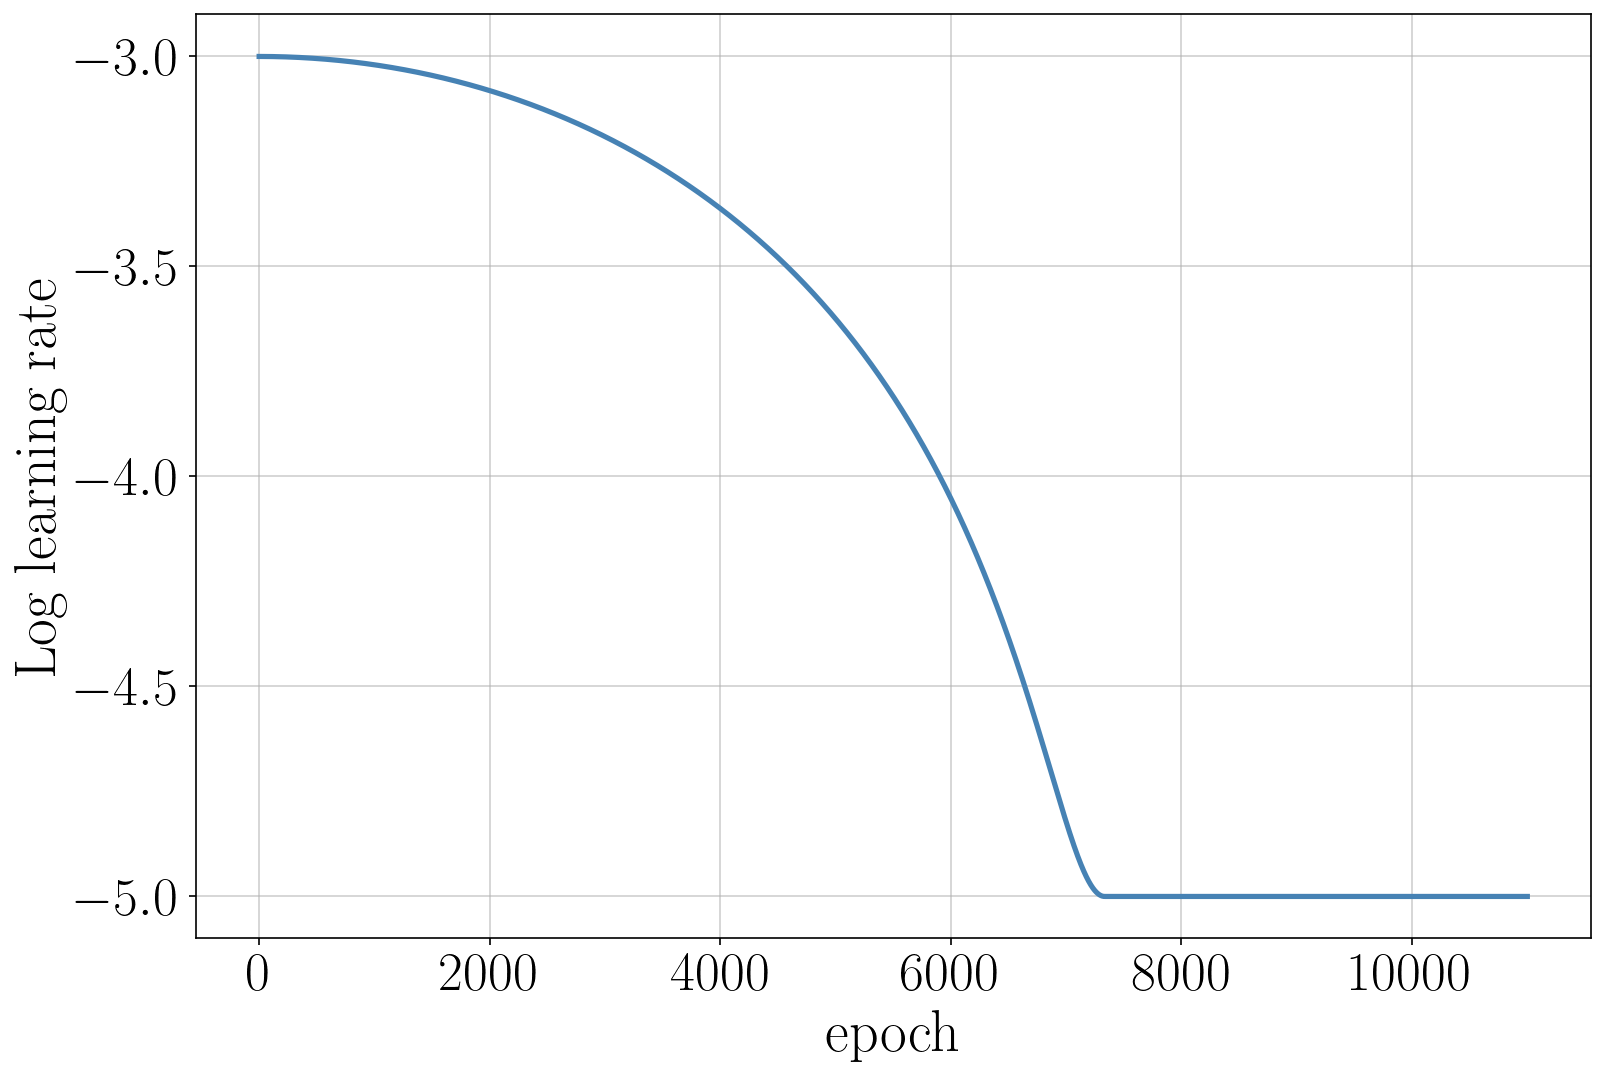
\includegraphics[width=0.6\linewidth]{figures/network_setup/lr}
	\caption{The evolution of the learning rate with each epoch on a logarithmic scale.}
	\label{fig:lr}
\end{figure}


% conclusion
\pageshift
%\thispagestyle{plain}
%\Section{Conclusion}
\label{sec:conclusion}

Since its discovery in 2012, the continuous research on the Standard Model (SM) Higgs boson has proven to be a fruitful endeavour. In order to constrain the Beyond the Standard Model nature of its coupling to known SM particles, several SM testing measurements have been performed, some of which require innovative analysis techniques.\\

In this thesis, inference on signal strength modifier parameters with cINNs at the CMS experiment has been discussed in detail. Thanks to their unique feature of being able to infer the true posterior distribution conditioned on observables directly, these networks are capable of reconstructing physics parameters correctly. In addition to that, Bayesian inference upon successful training takes several orders of magnitude less time than model fits based on frequentist approaches. Several proposed novel analysis approaches require the gradient of the observables to be propagated by such networks; as cINNs are built upon normalizing flows, the diffeomorphism encoded in the network model fulfils this property.\\

The gluon-fusion induced ZH production channel is a suitable candidate to look BSM effects for due to the loop-induced nature of the process at leading order. Using the measurable cross section of the quark initiated ZH and WH production processes, the observable $R^{ZW}_R$ can be measured by extracting the three signal processes from data via a likelihood fit.\\

In has been shown that the signal strength modifier parameters obtained from the likelihood fit can be inferred by the cINN model. Inference has been performed on the DNN probability scores for the three signal processes, 13 background nuisance parameters and one normalizing uncertainty, the luminosity. With that, the resulting network model had 17 dimensional inputs of physics parameters and a 235 dimensional condition input as physics observables on which the posteriors are conditioned on.

The study has been performed on simulated events exclusively. The training data has been constructed to reflect the expected statistical and systematic effects in measured data. For the former, both the limited MC sample size and the expected Poisson effects in the data have been taken into account. The shape-changing systematic effects are computationally expensive to simulate. For this reason, a non-linear histogram interpolation method (morphing) has been implemented to inter- and extrapolate among histogram templates. \\

Upon training, inference has been performed on the SM expectation. The obtained values for the signal process were

\begin{equation*}
		\mu_\text{ggZH} = 5.10^{+3.57}_{-3.50}, \, \, \quad \mu_\text{ZHDY} = 3.90^{+2.62}_{-2.57}, \, \, \quad \mu_\text{WH} = 3.02^{+1.92}_{-1.90} 
\end{equation*}

The sensitivity of the network with respect to different signal regions and physics processes has been discussed in detail. It has been shown that the network model does not have inherent biases due to wrong initialization or training relics. Rather, the network returns broad posteriors in regions of low sensitivity as expected. In addition to that, the network returns the prior distribution for unrecognized processes. It has been noted that the network cannot be more sensitive then the analysis itself.

% appendix
%\begin{appendix}
%	% appendix sections should look like this
%	 \pageshift
%	 \thispagestyle{plain}
%	 \Section{Foo}\label{sec:apx_foo}
%	 Foo.
%\end{appendix}


% bibliography
\linespread{1.0}\selectfont
\pageshift
\thispagestyle{plain}
\renewcommand{\headrulewidth}{0pt}
\renewcommand{\refname}{Bibliography}
\phantomsection
\addcontentsline{toc}{section}{Bibliography}
\bibliography{bib/bib}

% finalize thesis content
\renewcommand{\headrulewidth}{0pt}
\fancyhead{}
\fancyfoot{}

% thesis statement
\pageshift
\thispagestyle{empty}
\section*{Selbst\"andigkeitserkl\"arung}

Hiermit versichere ich an Eides statt, dass ich diese Arbeit einschlie\ss lich evtl. beigef\"ugter Abbildungen, Zeichnungen u.\"A.m. selbstst\"andig angefertigt und keine anderen als die angegebenen Hilfsmittel und Quellen benutzt habe. Alle Stellen, die dem Wortlaut oder dem Sinn nach anderen Werken entnommen sind, habe ich in jedem einzelnen Fall unter genauer Angabe der Quelle deutlich als Entlehnung kenntlich gemacht.\\
%
\vspace{1cm}
\\
{Aachen, den \handindate}\hfill
\begin{tabular}{c}
	\\\\\hline
	\hspace*{24mm}\author\hspace*{24mm}
\end{tabular}


% acknowledgment
\pageshift
\thispagestyle{empty}
\selectlanguage{ngerman}
\section*{Danksagung}

Thx.

